% (c) 2017 Leonardo Aldegheri
% (c) 2017 Carlotta Gualtieri

\input{\folder funzioni_grafici.tex}

\chapter{Introduzione alle funzioni}

\section{Cos'è una funzione}
\label{sec:funzioni2_cose}

In italiano la parola  ``funzione'' ha una decina di significati diversi: 
controllate su un buon vocabolario. Deriva dall latino:  ``functum'' che 
significa  ``eseguito''.
Possiamo pensare a una funzione come a un meccanismo che è in grado di 
eseguire un compito e dare quindi un risultato.

\begin{definizione}
 Chiameremo \textbf{funzione} la descrizione di un qualunque 
 \emph{processo} che dia un \emph{risultato}.
\end{definizione}

\begin{itemize} [noitemsep]
 \item Con \emph{processo} intendiamo un qualsiasi \emph{meccanismo} o 
\emph{procedimento} o \emph{algoritmo} o \emph{formula}...
 \item Con \emph{risultato} intendiamo un qualunque \emph{oggetto} prodotto 
dal \emph{processo}.
\end{itemize}

Il risultato viene anche chiamato \emph{output} della funzione.
 
\begin{esempio}
Vediamo qualche esempio che possa chiarire le idee \dots o confonderle 
ulteriormente.
\begin{itemize} [noitemsep]
 \item Una \emph{moka} è un meccanismo che produce una bevanda scura e 
molto calda.
 \item Un \emph{calcolo} è un meccanismo che produce un risultato numerico.
 \item Un \emph{bollitore} è uno strumento che produce acqua bollente.
 \item La \emph{media}  di più numeri è un meccanismo che produce un numero.
 \item Una \emph{stampante} è uno strumento che produce fogli scritti.
\end{itemize}
\end{esempio}

\subsection{Argomenti di una funzione}
\label{subsec:funzioni2_argomenti}

Una \emph{moka}, per quanto sofisticata sia, non ha la possibilità di 
produrre del caffè se non le vengono forniti dei  ``materiali":
\begin{itemize} [noitemsep]
 \item acqua,
 \item caffè tostato e macinato,
 \item calore.
\end{itemize}

 Questi  ``oggetti'' che la funzione usa e trasforma per dare il risultato 
vengono chiamati \emph{argomenti} della funzione.
 
Diamo quindi la seguente:

\begin{definizione}
 Chiamiamo \textbf{argomenti} gli oggetti che vengono passati ad 
una funzione e che la funzione può adoperare per dare un risultato.
\end{definizione}

Gli argomenti sono anche detti \emph{input} della funzione.

\paragraph{Riassumendo}

\begin{enumerate} [noitemsep]
 \item Una \emph{funzione} è un qualsiasi meccanismo che dà un 
\emph{risultato}.
 \item Il risultato è anche detto \emph{output} della funzione.
 \item Una funzione può essere chiamata passandole degli \emph{argomenti}.
 \item Gli argomenti di una funzione sono anche detti gli \emph{input} 
della funzione.
 \item Quindi, in generale, una funzione riceve degli \emph{oggetti} detti 
argomenti (o input) e produce un oggetto detto risultato (o output).
\end{enumerate}

\section{Costruiamo funzioni}
\label{sec:funzioni2_costruiamo}

Pr poter fare molti esperimenti e realizzare funzioni in modo economico e 
sicuro, in questo capitolo creeremo funzioni che lavorano su *simboli* cioè 
funzioni che prendono come argomenti dei simboli e producono come risultato 
dei simboli.

Potremo eseguire noi stessi la funzione o farla eseguire a un computer 
scrivendola in un linguaggio di programmazione. 
Nel seguito useremo il linguaggio Python che permette di scrivere funzioni 
facilmente comprensibili dagli umani e eseguibili in modo automatico da un 
computer.

Vediamo ora come realizzare alcune funzioni Python:

\begin{esempio}
 Scrivi la funzione che dia come risultato la stringa  ``ciao''.
 
\lstinputlisting{\folder src/01_saluto.py} %[firstline=2, lastline=5]
\end{esempio}

\begin{osservazione}
 \begin{enumerate} [nosep]
  \item Per definire una funzione, in Python,  dobbiamo usare:
  \begin{enumerate} [noitemsep]
   \item la parola riservata  ``def'', seguita dal
   \item nome della funzione (in questo caso  ``saluto'', ma avremmo potuto 
anche usare la parola  ``arggh"), seguito da una
   \item coppia di parentesi, seguite da
   \item il simbolo *duepunti* (":"), poi, a capo e rientrato
   \item un blocco di istruzioni, che termina con
   \item il comando  ``return'', seguito da
   \item il risultato della funzione.
  \end{enumerate}

  È più difficile da descrivere che da fare!
  Con i simboli possiamo riassumere la sintassi della definizione di una 
funzione in questo modo:
\begin{lstlisting}
  def <nome_funzione>():
       ``""<docstring>"""
      [<istruzioni>]
      return <risultato>
\end{lstlisting}

  \item Il testo posto come prima istruzione della funzione si chiama 
\emph{docstring} e descrive in modo sintetico cosa fa la funzione.
  \item Per eseguire una funzione dobbiamo chiamare il nome della funzione 
seguita da una coppia di parentesi.
\begin{lstlisting}
  <nomefunzione>()
\end{lstlisting}
  \item Nella descrizione della sintassi:
  \begin{enumerate} [nosep]
   \item le parti tra parentesi angolari ("<'' e  ``>") vanno sostituiti 
con 
qualcosa di sensato;
   \item le parti tra parentesi quadrate ("['' e  ``]") sono opzionali.
  \end{enumerate}
 \end{enumerate}
\end{osservazione}

\begin{esempio}
 Scrivi la funzione che dia come risultato la media di due numeri.

Questa volta, la funzione deve ricevere due argomenti per poter dare il suo 
risultato. Vediamo come realizzarla.

\lstinputlisting[lastline=5]{\folder src/02_media.py} %[firstline=2, 
lastline=5]
\end{esempio}

\begin{osservazione}
 \begin{enumerate} [nosep]
  \item La coppia di parentesi che segue il nome della funzione nella 
definizione contiene due nomi. Questi nomi vengono detti *parametri* della 
funzione.
  \item La funzione precedente non aveva parametri, questa funzione ha 2 
parametri.
  \item La sintassi completa di una funzione è:
\begin{lstlisting}
  def <nome_funzione>([<parametri>]):
       ``""<docstring>"""
      [<istruzioni>]
      return <risultato>
\end{lstlisting}
  \item Se la funzione ha 2 parametri, per eseguirla dovrò fornirle 2 
argomenti. 
Quindi per eseguirla, dovrò mettere tra parentesi due oggetti che verranno 
collegati ai due parametri:
\begin{lstlisting}
  <nomefunzione>([<argomenti>])
\end{lstlisting}
 \end{enumerate}
\end{osservazione}

Prova a eseguire la precedente funzione passandole diversi argomenti.
\lstinputlisting[firstline=7]{\folder src/02_media.py} %[, lastline=5]

\begin{osservazione}
Osservate la differenza tra la media dei due numeri 34 e 56 e la media 
tra 0.34 e 0.56. La cosa risulta strana, ma dipende dal fatto che molti 
numeri che per noi sono decimali limitati, per il computer sono decimali 
periodici. e quindi sono *sempre* approssimati.
\end{osservazione}

\begin{esempio}
Scrivi la funzione che dia come risultato la lunghezza di una stringa.

\begin{osservazione}
Intendiamo con *stringa* una sequenza di caratteri cioè una parola o 
un testo.
\end{osservazione}

\lstinputlisting{\folder src/03_lunghezza.py} %[, lastline=5]

Prova a eseguire la precedente funzione passandole diversi argomenti.
\end{esempio}

\begin{esempio}
Scrivi la funzione che dia come risultato il terzo carattere di una 
stringa.

\lstinputlisting{\folder src/04_terzocarattere.py} %[, lastline=5]

Prova a eseguire la precedente funzione passandole diversi argomenti.
\end{esempio}

\begin{osservazione}
 A tutte le persone normali potrà sembrare strano che per ottenere il 
terzo carattere si debba mettere tra le parentesi quadre il numero 2. 
La cosa si spiega considerando che in Python (e non solo in Python) le 
sequenze iniziano dal numero zero. Quindi il primo carattere è quello che 
ha posizione 0, il secondo quello che ha posizione 1 e il terzo quello che 
ha posizione 2.
\end{osservazione}

\begin{esempio}
Scrivi la funzione che dia come risultato *vero* se un numero è pari e 
*falso* se un numero è dispari.

\lstinputlisting{\folder src/05_pari.py} %[, lastline=5]

Prova a eseguire la precedente funzione passandole diversi argomenti.
\end{esempio}

\begin{osservazione}
 \begin{enumerate} [nosep]
  \item Il simbolo ``\%'' rappresenta l'operazione che dà come risultato il 
resto della divisione tra i suoi operandi.
  \item Il simbolo ``=='' rappresenta l'operazione di confronto 
dell'uguaglianza: 
dà come risultato \emph{True} se i suoi operandi sono uguali, \emph{False} 
in caso contrario.
  \item Un numero è pari se il resto della divisione per 2 è zero.
  \item L'argomento della funzione deve essere un numero.
  \item Il risultato è un elemento dell'\emph{insieme bouleano}: {False, 
True}.
 \end{enumerate}
\end{osservazione}

\section{Argomenti, Dominio e Insieme di Definizione}
\label{sec:funzioni2_dominio}

Se nel fare gli esperimenti con le funzioni definite precedentemente siete 
stati un po' creativi, potreste aver provato qualcosa del genere:

\begin{lstlisting}
print(lunghezza("otto"))
print(lunghezza(8))
\end{lstlisting}

Evidentemente la funzione accetta come argomento la stringa  ``otto'', ma 
non il numero 8.

Possiamo ottenere errori anche nell'esecuzione della funzione media:

\begin{lstlisting}
print(media(3, 10))
print(media("tre'',  ``dieci"))
\end{lstlisting}

In questo caso la funzione vuole avere dei numeri non delle stringhe, anche 
se rappresentano dei numeri.

Per descrivere una funzione in modo da poterla usare con sicurezza 
dobbiamo indicare anche l'insieme di oggetti che possono essere passati 
alla funzione come parametri. Questo insieme viene chiamato 
\textbf{dominio}.

\begin{definizione}
Chiameremo \textbf{dominio}  di una funzione l'insieme degli elementi che 
possono essere suoi argomenti.
\end{definizione}

Cioè il \emph{tipo} degli oggetti a cui la funzione può essere applicata.

Quindi, riferendoci alle funzioni definite precedentemente:

\begin{enumerate} [noitemsep]
\item Il dominio della funzione \texttt{lunghezza} è l'insieme delle 
stringhe; cioè la funzione \texttt{lunghezza} può essere applicata agli 
oggetti ti tipo stringa.
\item Il dominio della funzione \texttt{triplo} è l'insieme dei numeri.
\item Il dominio della funzione \texttt{media} è l'insieme delle coppie di 
numeri.
\item Il dominio della funzione \texttt{terzo\_carattere} è l'insieme delle 
stringhe.
\item Il dominio della funzione \texttt{primo\_carattere} ...
\item Il dominio della funzione \texttt{somma}...
\item \emph{Completa scrivendo il dominio delle altre funzioni proposte.}
\end{enumerate}

Nel fare esperimenti dovresti aver individuato che il dominio della 
funzione \texttt{terzo\_carattere} è l'insieme delle stringhe. Ma non tutte 
le strighe vanno bene:

\begin{lstlisting}
print(terzo_carattere("ba"))
\end{lstlisting}

Effettivamente, chiedere di restituire il terzo carattere di una parola 
formata solo da 2 caratteri è un po' pretenzioso!

La funzione viene sì applicata alle stringhe, ma non 
tutte le stringhe vanno bene: solo quelle con almeno 3 caratteri. 
Possiamo dire che gli argomenti di questa funzione devono essere delle 
stringhe (\emph{dominio}) ma le stringhe per le quali la funzione è 
definita sono solo quelle con almeno 3 caratteri 
(\emph{insieme di definizione}).

\begin{definizione}
Chiameremo \textbf{insieme di definizione}  di una funzione, il 
sottoinsieme del \emph{dominio} formato dagli elementi che permettono di 
calcolare un risultato.
\end{definizione}

L'\emph{insieme di definizione} o \emph{insieme di esistenza} di una 
funzione è il sottoinsieme degli elementi del dominio che non danno un 
errore quando vengono usati come argomento della funzione.

\section{Risultato, Codominio e Insieme Immagine}
\label{sec:funzioni2_codominio}

\begin{definizione}
Chiamiamo \textbf{codominio} un'insieme che contiene tutti i risultati di 
una funzione.
\end{definizione}

Cioè il codominio è il \emph{tipo} di risultato della funzione.

Ma anche in questo caso non tutti gli elementi del codominio possono essere 
effettivamente risultati di una funzione, se consideriamo solo questi 
elementi otteniamo un sottoinsieme del codominio:

\begin{definizione}
Chiamiamo \textbf{insieme immagine} di una funzione il sottoinsieme del 
codominio che contiene solo i risultati di una funzione.
\end{definizione}

\begin{esempio}
Determina: Dominio, Insieme di Definizione, Codominio e Insieme Immagine 
della funzione: \texttt{terzocarattere} 

Il dominio è costituito dalle stringhe; l'insieme di definizione è il 
sottoinsieme delle stringhe che hanno almeno~3 caratteri; il Codominio è 
formato dall'insieme delle stringhe; l'Insieme Immagine è il sottoinsieme 
delle stringhe di lunghezza~1.
\end{esempio}

\begin{osservazione}
\paragraph{``Unicità'' del risultato}

In generale ci aspettiamo che una funzione dia un risultato ben preciso:
\begin{itemize} [nosep]
 \item la metà di 13 è 6,5;
 \item la media tra 20 e 30 è 25;
 \item l'ultima lettera della parola  ``Mah'' è  ``h";
 \item \dots
\end{itemize}

Non ci aspettiamo che la metà di 13 sia a volte un numero, a volte un altro 
numero o sia un insieme di numeri.

Non è detto che una funzione debba per forza restituire un solo numero, 
potrebbe restituire un intervallo di numeri o un insieme di numeri o di 
oggetti.

Non è neppure detto che una funzione debba restituire sempre lo stesso 
numero, ad esempio una funzione che dia come risultato un numero casuale 
restituirà alle volte un numero, altre volte un altro numero.

Comunque, ogni volta che usiamo una certa funzione, otteniamo un preciso 
risultato che tutti siamo d'accordo di accettare.
\end{osservazione}

\subsection{Altre convenzioni}

È importante notare che altri testi, la maggioranza in verità, non usano 
questa convenzione ma un'altra:

\begin{itemize} [nosep]
 \item quello che noi chiamiamo ``dominio'' viene chiamato  ``insieme A'', 
o in 
qualche altro modo;
 \item quello che chiamiamo ``codominio'' viene chiamato  ``insieme B'', o 
in qualche altro modo;
 \item quello che chiamiamo ``insieme di definizione'' viene chiamato 
``dominio'';
 \item quello che chiamiamo ``insieme immagine'' viene chiamato 
``codominio''.
\end{itemize}

Bisogna capire dal contesto il significato dei termini, ad esempio, se 
viene chiesto di trovare il ``dominio di una funzione reale'', è evidente 
che ci viene chiesto di trovare quello che noi chiamiamo ``insieme di 
definizione'' dato che per noi il dominio di una funzione reale è, per 
definizione, $\mathbb{R}$.

Attento a distinguere i concetti fondamentali dai nomi usati per 
esprimerli: una volta capiti i concetti. Per accordarci sui nomi basta una 
penna: tirare un segno sul nome da cambiare e scrivere vicino il nuovo nome.

\section{Rappresentazione di una generica funzione}
\label{sec:funzioni2_rappresentazione}

\subsection{Diagrammi}

Quanto detto può essere rappresentato dalla seguente figura dove gli 
insiemi di partenza e di arrivo sono visualizzati con i diagrammi di 
Eulero-Venn e la regola che collega gli elementi dell'insieme di definizione 
con gli elementi dell'insieme immagine è indicata con una freccia.

\begin{center}
\deffunzione{Dominio}{Insieme di Definizione}{Codominio}{Insieme Immagine}
\end{center}

\subsection{Notazioni matematiche}

Se chiamiamo $y$ il risultato della funzione 

Possiamo indicare che $y$ è il risultato di una funzione con la seguente 
espressione matematica:

$$y=f(x)$$

Ad esempio se la funzione restituisce la metà del quadrato di un numero la 
funzione può essere scritta:

$$y=\frac{1}{2}x^2$$

Altra notazione per indicare una funzione è:

$$f: x \mapsto f(x)$$

Usando sempre l'esempio precedente:

$$f: x \mapsto \frac{1}{2}x^2$$

In Python la funzione $f$ può essere creata usando il costrutto 
``def \dots return \dots'' o la funzione ``lambda``:


\begin{lstlisting}
def f(x):
    return 1/2*x**2

f = lambda x: 1/2*x**2
\end{lstlisting}

\begin{osservazione}
La lettera $f$ viene usata per indicare una generica funzione. 
Quando dobbiamo, nello stesso discorso, indicare altre generiche funzioni, 
di solito vengono usate altre lettere dell'alfabeto vicine alla effe: $g$, 
$h$, ...

Invece, $k$ di solito viene usata per indicare una funzione costante, cioè 
una funzione che dà sempre lo stesso risultato qualunque sia l'argomento.
\end{osservazione}

\paragraph{Riassumendo}

\begin{enumerate} [noitemsep]
\item Chiamiamo \emph{funzione} un qualunque procedimento che può avere 
degli argomenti e che dà un risultato che tutti accettiamo.
\item Una funzione viene applicata a un limitato insieme di oggetti questo 
insieme è detto \emph{dominio}.
\item Gli elementi del dominio che possono essere calcolati, senza dare 
errori, formano l'\emph{Insieme di Definizione} della funzione.
\item Una funzione ha risultati che appartengono ad un determinato insieme, 
questo insieme è detto \emph{codominio}.
\item Il sottoinsieme del codominio che è costituito dagli elementi che 
possono essere effettivamente il risultato della funzione, formano 
l'\emph{Insieme Immagine} della funzione.
\end{enumerate}

\section{Funzioni reali}
\label{sec:funzioni2_reali}

Abbiamo visto che possiamo avere funzioni applicate a moltissimi insiemi e 
con i più vari risultati; possono essere semplici, descritte da un semplice 
calcolo o complicate descrivibili solo con un gran numero di righe.

Noi siamo all'inizio dello studio delle funzioni per cui ci 
semplifichiamo un po' la vita restringendo l'insieme delle funzioni da 
studiare al sottoinsieme delle sole funzioni che partono da un numero e 
danno come risultato un numero. 
Tra i vari insiemi di numeri che possiamo usare scegliamo l'insieme dei 
numeri reali: $\mathbb{R}$. Scegliamo i reali perché hanno meno restrizioni 
rispetto ad altri e perché hanno un semplice modello facile da realizzare: 
la \emph{retta reale} (un asse cartesiano).

Chiameremo queste le \emph{funzioni reali} o 
\emph{funzioni reali di variabili reali}.

\begin{definizione}
Chiamiamo \emph{funzioni reali di variabili reali} o, più 
semplicemente, \emph{funzioni reali} le funzioni che hanno per dominio e 
per codominio i numeri reali.
\end{definizione}

\begin{esempio}
Come esempio potremmo scrivere la funzione che dà come risultato la metà di 
un numero aumentata di 3:

\lstinputlisting[lastline=7]{\folder src/07_metapiutre.py} %]

\end{esempio}

Andando avanti, dovremmo scrivere molte funzioni, non sempre potremmo 
scrivere un nome che rispecchi esattamente quello che fa la funzione stessa 
per cui sarà il caso che usiamo dei nomi più generici e semplici. 
La funzione precedente può essere scritta così:

\lstinputlisting[firstline=9]{\folder src/07_metapiutre.py} %]

\subsection{Tabella di alcuni valori di una funzione}

Negli esempi precedenti ci siamo fatti stampare il valore assunto dalla 
funzione per alcuni valori del suo argomento ma se avessimo bisogno di più 
valori, il metodo precedente sarebbe piuttosto scomodo. Possiamo scrivere 
una funzione che non dà risultato, ma, data una funzione e un insieme di 
numeri, stampa ognuno dei numeri seguito dal risultato della funzione 
applicata a quel numero:

\lstinputlisting[lastline=9]{\folder src/08_tabelle.py} %]

Oppure se è più comoda una tabella orizzontale, stampa prima gli 
argomenti e sotto i corrispondenti risultati della funzione:

\lstinputlisting[firstline=10]{\folder src/08_tabelle.py} %]

\begin{osservazione}
Per capire le funzioni, non è importante capire come funziona la funzione 
\texttt{tabella} o la funzione \texttt{tabella\_o}.
Se sei curioso puoi cercare di capirle, altrimenti puoi usarle senza porti 
tanti problemi.
\end{osservazione}

\subsection{Scrittura matematica}

In matematica la funzione precedente viene scritta in uno di questi modi:

$$f_0(x) = \frac{1}{2}x +3 \quad \text{ o } \quad 
y= \frac{1}{2}x +3 \quad \text{ o } \quad 
f: x \mapsto \frac{1}{2}x +3$$

Osservando la tabella precedente possiamo formulare alcune congetture:

\begin{enumerate} [nosep]
\item Ogni volta che $x$ aumenta di 1, $f_0(x)$ aumenta di $\frac{1}{2}$.
\item Se $x$ aumenta anche $f_0(x)$ aumenta.
\item Se $x$ diminuisce anche $f_0(x)$ diminuisce.
\end{enumerate}


\subsection{Visualizzazione su due assi}

Una funzione reale fa corrispondere ad un numero un altro numero, ma i 
numeri possono essere visualizzati su una retta, un asse cartesiano. 
Possiamo quindi rappresentare la funzione come una corrispondenza tra i 
punti di due rette.

Chiamiamo $x$ la retta da cui partono le frecce e $y$ la retta su cui le 
frecce arrivano.
Sulla retta $x$ rappresenteremo gli argomenti della funzione e sulla retta 
$y$ i corrispondenti risultati.

\dueassivuoti

Vediamo alcuni esempi, partendo da funzioni molto semplici e complicando, 
man mano, le cose.

\begin{esempio}
Calcola e rappresenta la funzione che dato un numero restituisce lo stesso 
numero aumentato di tre.

\lstinputlisting[lastline=3]{\folder src/09_funzioni.py} %]

Collegando i punti corrispondenti nel grafico con due assi otteniamo:

\dueassi{-13}{10}{\x+3}
\end{esempio}


\begin{osservazione}
\begin{enumerate}
\item La funzione è definita anche per valori diversi da quelli per i quali 
abbiamo fatto stampare la tabella.
\item È definita anche per valori diversi da quelli che abbiamo 
rappresentato nel grafico.
\item Solo per motivi di pigrizia abbiamo usato come argomenti numeri 
interi, ma la funzione è definita anche per qualunque altro numero reale.
\end{enumerate}
\end{osservazione}

\section{Rappresentazione cartesiana}
\label{sec:funzioni2_rcartesiana}

La visualizzazione su due assi ha il pregio di mettere bene in evidenza il 
collegamento tra l'argomento e il risultato di una funzione, ma, se la 
funzione non è semplicissima, può facilmente diventare un guazzabuglio di 
frecce, un grafico a spaghetti difficilmente interpretabile. Non si presta 
certo a rendere il significato di una funzione a colpo d'occhio.

La trovata geniale è stata quella di ruotare di 90 gradi l'asse delle $y$ e 
di indicare la relazione tra l'*argomento* e il *risultato* con un *punto*:

\puntonelpc{2}{5}

\begin{osservazione}
\begin{enumerate} [nosep]
\item Per pigrizia, al posto di  ``argomento'' e di  ``risultato'', 
normalmente si usano due lettere:  ``x'' e  ``y''.
\item Il punto P rappresenta una coppia di valori  ``argomento'' -  
``risultato''.
\item È possibile rappresentare l'intera funzione disegnando tutti i punti, 
solitamente infiniti.
\item L'insieme di tutti questi punti viene detto grafico della funzione.
\item Di solito ci si accontenta di rappresentare una parte della funzione, 
quella che si ritiene più significativa.
\end{enumerate}
\end{osservazione}

\subsection{Grafico di una funzione}

Riportiamo nel piano cartesiano i punti che hanno per coordinate gli 
argomenti e risultati della funzione 
$\quad f_6: x \mapsto -2x+3 \quad$ 
ricavati dalla tabella precedente:

\begin{lstlisting}
tabella_o(lambda x: -2 * x +3, range(-4, +7))
\end{lstlisting}


"""Vediamo come appare il grafico della funzione:

$$f_6: x \mapsto -2x+3$$

Riportiamo nel piano cartesiano i punti che hanno per coordinate gli 
argomenti e risultati della funzione ricavati dalla tabella precedente:

\graficoa

\begin{osservazione}
\begin{enumerate}
\item Nel grafico vengono disegnati alcuni punti che hanno per coordinate 
l'argomento e il risultato della funzione.
\item Se calcoliamo la funzione nei valori intermedi a quelli rappresentati 
vedremo che i punti ottenuti si disporranno tra quelli già rappresentati. 
\end{enumerate}
\end{osservazione}

Ad es. 
$f(0,5)=2$, $f(0,75)=2,5$, $f(0,25)=1,5$, ...

Possiamo aggiungere facilmente i punti intermedi, anzi possiamo aggiungere 
facilmente *infiniti* punti semplicemente collegando quelli già disegnati 
con una linea. Inquesto caso una linea retta:

\graficob

\begin{osservazione}
Questa rappresentazione fa emergere una caratteristica che finora non 
potevamo sospettare: la funzione ha una sua forma. In questo caso, la 
funzione ha la forma di una retta decrescente che taglia l'asse y nel punto 
$3$.

La forma della funzione viene chiamata: *grafico della funzione*.
\end{osservazione}

\subsection{Disegnare grafici con Python}

Di seguito la funzione Python che disegna il grafico della funzione passata 
come argomento.

\lstinputlisting{\folder src/10_assiegrafico.py} %]

\begin{osservazione}
Anche in questo caso la funzione che disegna il grafico appare piuttosto 
complicata, non è necessario capire come funziona.
L'ultima riga della cella precedente indica come chiamarla, questa è la 
parte importante.

Per studiare invece il funzionamento della funzione ``grafico`` la strada 
più semplice è quella di fare delle modifiche e vederne l'effetto.
\end{osservazione}

% \begin{lstlisting}
% grafico(lambda x: -x**2+8)
% \end{lstlisting}


\paragraph{Riassumendo}

\begin{itemize} [nosep]
\item È possibile rappresentare alcune coppie *argomento* - *risultato* con:
\begin{itemize} [nosep]
  \item una tabella,
  \item delle frecce che uniscono i punti di due assi cartesiani,
  \item un insieme di punti nel piano cartesiano
\end{itemize}
\item La rappresentazione cartesiana permette di associare ad ogni funzione 
una forma ben precisa.
\end{itemize}



\subsection{}


\section{}
\label{sec:funzioni2_}



\begin{comment}
%--------------------------------------------------------------------
% Per inserire codice

\section{}
\label{sec:funzioni2_}

\label{sec:funzioni2_dominio}

\lstinputlisting[firstline=2, lastline=5]{\folder src/.py} %]

\begin{lstlisting}
\end{lstlisting}

\begin{definizione}
\end{definizione}

\begin{esempio}
\end{esempio}

\begin{osservazione}
\end{osservazione}
%--------------------------------------------------------------------

## Proprietà delle funzioni

### Iniettiva

**Definizione** 

Una funzione si dice **iniettiva** se a elementi di versi dell'insieme di 
definizione corrispondono elementi diversi dell'insieme immagine.
$$\forall x_1, x_2, \quad \text{se} \quad x_1 \ne x_2 
\quad \text{allora} \quad f(x_1) \ne f(x_2)$$

**Esempio**

La funzione $\quad y = 3x-2 \quad$ è iniettiva perché lo stesso $y$ non può 
essere prodotto da duiversi $x$.
"""

grafico(lambda x: 2**(x+1))

"""**Controesempio**

La funzione $\quad y = x^2-2 \quad$ non è iniettiva perché lo stesso $y$ 
può 
essere prodotto da duiversi $x$.
"""

grafico(lambda x: x**2 -2)

"""In questo caso, ad esempio, il risultato $7$ è prodotto sia da $-3$ sia 
da $+3$.

### Suriettiva

**Definizione** 

Una funzione si dice **suriettiva** se l'insieme immagine coincide con il 
codominio.

**Esempio** 

La funzione $\quad y= x^3 -4x \quad$ è suriettiva perché ogni valore reale 
$y$ può essere generato da almeno un valore di $x$:
"""

grafico(lambda x: x**3 -4*x)

"""**Controesempio**

La funzione $\quad y = - e^x \quad$ non è suriettiva perché nessun valore 
positivo può essere generato da questa funzione.
"""

grafico(lambda x: -np.exp(x))

"""### Biiettiva

**Definizione** 

Una funzione si dice **biiettiva** se è iniettiva e suriettiva.

**Esempio**

La funzione $\quad y = x^3+2 \quad$ è biiettiva perché ogni valore di $y$ è 
generato da uno e un solo valore di $x$.
"""

grafico(lambda x: x**3+2)

"""**Controesempio**

Tutti gli esempi dei paragrafi precedenti.

# Caratteristiche di una funzione

Data una funzione in forma matematica è possibile determinare alcune sue 
proprietà in modo abbastanza semplice, per altre servono degli strumenti 
matematici che ancora non conosciamo.

## Monotonia

Con il termine  ``monotòna'' (diversa da  ``monòtona") intendiamo una 
funzione 
che ha lo stesso andamento, cioè che è crescente o decrescente.

### Crescente 

Una funzione è crescente se all'aumentare dell'argomento ($x$) aumenta 
anche 
il risultato ($y$). Se questo è vero per tutte le $x$ dell'insieme di 
definizione allora diremo che la funzione è monotòna crescente.

---
**Definizione**
Una funzione si dice *monotona crescente* se ad argomenti più grandi 
corrispondono risultati più grandi (se all'aumentare di $x$ aumenta anche  
$f(x)$):

$$\forall x_0, x_1 \in \mathbb{IE} ~\land~ x_1 > x_0 ~\Rightarrow~ 
f(x_1) > f(x_0)$$

---

**Osservazione**

È del tutto equivalente dire che una funzione è *crescente* se ad 
*argomenti 
più piccoli* corrispondono *risultati più piccoli*.

---

Esempio di funzione crescente:
"""

grafico(lambda x: np.log2(x))

"""---

**Osservazione**

Otteniamo una strana scritta prima che ci venga visualizzato il grafico: 
Python ci avvisa che ha fatto tutti i calcoli necessari per disegnarlo, ma 
che ha incontrato dei valori non validi nelle'eseguire  ``log2''. Sapresti 
dare 
una spiegazione di questo avviso?

---

Facciamo stampare  la tabella di alcune coppie argomento-risultato per la 
funzione *log2*.
"""

tabella(lambda x: np.log2(x), [x/2 for x in range(-10, 10)])

"""Otteniamo ancora strani messaggi e, tra i risultati, otteniamo delle 
scritte che non sono un numeri...  

Se ripensiamo al significato di *logaritmo* vediamo che l'espressione 
"log2(0)'' equivale a cercare l'esponente da dare a 2 per ottenere 0 cosa 
impossibile. E  ``log2(-4)'' equivale a cercare l'esponente da dare a 2 per 
ottenere -4 cosa altrettanto impossibile.

Ritornando al nostro problema:

### Esercizio

Verifica per almeno 3 coppie di valori di $x$ che se $x_1$ è maggiore di 
$x_0$ allora anche  $f(x_1)$ è maggiore di $f(x_0)$  e per altre 3 coppie 
di 
valori di $x$ che se $x_1$ è miore di $x_0$ allora anche  $f(x_1)$ è miore 
di $f(x_0)$.

### Decrescente 

Una funzione è *decrescente* se all'aumentare dell'argomento ($x$) 
diminuisce il risultato ($y$). Se questo è vero per tutte le $x$ 
dell'insieme di definizione allora diremo che la funzione è monotòna 
decrescente.

---
**Definizione**
Una funzione si dice *monotona decrescente* se ad argomenti più grandi 
corrispondono risultati più piccoli (se all'aumentare di $x$ diminuisce 
$f(x)$):

$$\forall x_0, x_1 \in \mathbb{IE} ~\land~ x_1 > x_0 ~\Rightarrow~ 
f(x_1) < f(x_0)$$

---

**Osservazione**

È del tutto equivalente dire che una funzione è decrescente se ad argomenti 
più piccoli corrispondono risultati più grandi.

---

Grafico di una funzione decrescente:
"""

grafico(lambda x: -.5*x+2)

"""### Intervalli di monotonia

Una funzione può essere crescente in certi intervalli di $x$ e decrescente 
in altri.

Uno dei problemi da risolvere quando ci sarà chiesto di studiare una 
funzione sarà quella di individuare gli intervalli di monotonia, cioè per 
quali valori di $x$ la funzione è crescente e per quali è decrescente.

---
**Esempio**

Individua gli intervalli di monotonia della funzione che ha il seguente 
grafico.

![Intervalli di 
monotonia]
(https://drive.google.com/uc?export=view&id=1w8Og5HxVbNz9tFL3-OcgZuzdpq2G8yG
L)

Possiamo immaginare che la funzione che ha questo grafico cresca fino a che 
$x$ vale $a$, decresca da $a$ a $b$, poi torni a crescere.

In $a$ e $b$ la funzione ha due *punti stazionari* e precisamente in $a$ la 
funzione ha un *massimo relativo* e in $b$ un *minimo relativo*.

**Osservazione**

È chiaro che possiamo dire qualcosa di abbastanza sicuro solo sulla parte 
del grafico che vediamo. In questo caso, su cosa faccia la funzione quando 
$x$ è più piccolo di $-6,5$ o più grande di $10$ possiamo fare solo delle 
ipotesi.

---

### Esercizi

Tra le seguenti funzioni individua quali sono crescenti, quali decrescenti 
e 
quali hanno dei tratti crescenti e dei tratti decrescenti.

\item $f_0: x \mapsto - \dfrac{8}{7} x$
\item $f_1: x \mapsto \dfrac{12}{x}$
\item $f_2: x \mapsto  \dfrac{2}{5} x -2$
\item $f_3: x \mapsto \dfrac{1}{2}x^2$
\item $f_4: x \mapsto - \dfrac{4}{3} x^2 -2$
\item $f_5: x \mapsto - \dfrac{3x-2}{2x+4}$

## Parità

La *parità* riguarda la simmetria della funzione rispetto all'asse $y$ o 
rispetto all'origine.

### Funzioni pari

Diremo che una funzione è pari se è simmetrica rispetto all'asse $y$, cioè 
a 
distanza uguale dall'asse ha valori uguali:

---
**Definizione**

Una funzione è *pari* se a valori opposti dell'argomento corrisponde lo 
stesso risultato:

$$f(-x) = f(x)$$

---

![Funzione pari](https://drive.google.com/uc?export=view&id=)
"""

grafico(lambda x: (x**3 -3*x)/(-2*x**3 +5*x))

tabella(lambda x: (x**3 -3*x)/(-2*x**3 +5*x), range(-10, 0))
tabella(lambda x: (x**3 -3*x)/(-2*x**3 +5*x), range(1, 11))

"""### Funzioni dispari

Diremo che una funzione è dispari se è simmetrica rispetto all'origine, 
cioè 
a distanza uguale dall'asse ha valori opposti:

---
**Definizione**

Una funzione è *dispari* se a valori opposti dell'argomento corrispondono 
risultati opposti:

$$f(-x) = -f(x)$$

---

![Funzione dispari](https://drive.google.com/uc?export=view&id=)
"""

grafico(lambda x: (x**3 - 6*x)/(x**2 + 4))

tabella(lambda x: (x**3 - 6*x)/(x**2 + 4), range(-10, 11))

"""Per verificare se una funzione è pari o dispari basta sostituire la 
variabile $x$ con il suo opposto: $-x$ e vedere se si ottiene una funzione 
equivalente a quella di partenza o al suo opposto:

**Esempi**

1\. Verifica la parità di: 
$\quad f: x \mapsto \dfrac{3x}{2x^2-4}$

Sostituendo otteniamo:

$$ f(-x) = \frac{3(-x)}{2(-x)^2-4} =
              \frac{-3x}{2x^2-4} =
              -\frac{3x}{2x^2-4} = -f(x)$$
              
Poiché $f(-x)=-f(x) (effe di meno x è uguale a meno effe di x), la funzione 
è dispari.

2\. Verifica la parità di: 
$\quad f: x \mapsto \dfrac{4x^4-3x^2}{2x^2-5}$

Sostituendo otteniamo:

$$ f(-x) = \dfrac{4x^4-3x^2}{2x^2-5} =
              \dfrac{4(-x)^4-3(-x)^2}{2(-x)^2-5} =
              \dfrac{4x^4-3x^2}{2x^2-5} =
              f(x)$$
              
Poiché $f(-x)=f(x) (effe di meno x è uguale a meno effe di x), la funzione 
è 
pari.

3\. Verifica la parità di: 
$\quad f: x \mapsto 4x^4-3x^2+5x$

Sostituendo otteniamo:

$$ f(-x) = 4(-x)^4-3(-x)^2+5(-x) =
              4x^4-3x^2-5x $$
              
Osservando attentamente i segni possiamo concludere che:
$$f(-x) \ne f(x) \quad \text{e} \quad f(-x) \ne -f(x)$$ 
              
Quindi $f(-x)$ non è né pari né dispari.

---
**Osservazioni**

\item Se una funzione è *pari*, basta studiarla solo per i valori positivi 
del 
suo Insieme di definizione.
\item *Mutatis mutandis* lo stesso vale per le funzioni *dispari*.

---

### Esercizi

Tra le seguenti funzioni individua quali sono pari, quali dispari e quali 
né 
pari né dispari.

\item $f_0: x \mapsto - x^4 +3x^2 -2$
\item $f_1: x \mapsto x^3-2x$
\item $f_2: x \mapsto x^4 - x^3$
\item $f_3: x \mapsto - \dfrac{6}{5} x$
\item $f_4: x \mapsto \dfrac{6}{x}$
\item $f_5: x \mapsto - \dfrac{5}{4} x -2$
\item $f_6: x \mapsto x^2$
\item $f_7: x \mapsto -x^2 + 7$
\item $f_8: x \mapsto - \dfrac{1}{2} x^2 -2x$
\item $f_9: x \mapsto - \dfrac{x-2}{3x+4}$

## Periodicità

Diremo che una funzione è periodica se, a intervalli regolari, si ripete 
sempre allo stesso modo:

---
**Definizione**

Una funzione è *periodica* se a distanza di un certo intervallo produce gli 
stessi valori.

Chiamando $i$ l'ampiezza dell'intervallo di periodicità $\mathbb{I}$:

$$\forall x \in \mathbb{I} \quad  f(x + i) = f(x)$$

---
**Osservazione**

Se una funzione è periodica, basta studiare solo un intervallo di 
periodicità.

---
"""

grafico(lambda x: np.sin(x)+2*np.sin(2*x))

"""Si può osservare che la funzione si ripete con un periodo che è 
leggeremente superiore a $6$, precisamente il periodo della funzione è: 
$2\pi$.

### Esercizi

## Zeri di una funzione

Si dicono *zeri di una funzione* i valori dell'argomento che producono $0$ 
come risultato.

---
**Definizione**

Diremo che $z$ è uno *zero* della funzione se $f(z) = 0$.

---

**Osservazioni**

\item Gli zeri di una funzione si trovano risolvendo l'equazione: $f(x) = 0$
\item Dato che l'asse $x$ ha equazione $y = 0$, gli zeri della funzione 
indicano i punti in cui il grafico della funzione interseca l'asse $x$.

---
**Esempio**

Calcola gli zeri della funzione: $f(x) = x^2 -3x - 10$

$x^2 -3x - 10=0 \quad \Rightarrow \quad \left(x-5 \right) 
\left(x+2\right)=0 
\quad \Rightarrow \quad x_0=-2 \text{ e }x_1=5$

Il grafico di questa funzione interseca l'asse $x$ nei punti: $-2$ e $5$.

---

### Esercizi

## Limitatezza

**Definizione**

Una funzione si dice **limitata** se la sua immagine ha un valore massimo e 
un valore minimo.

Si dice **illimitata** se la sua immagine non ha un massimo o non ha un 
minimo.

Possimo distinguere diversi casi di una funzione $f$ definita in un 
intervallo $\mathbb{I}$:

* **Limitata superiormente** se la sua immagine ha un estremo superiore:
$$\exists k \in \mathbb{R} ~|~ \forall x \in \mathbb{I}, \quad f(x) \le k$$
* **Limitata inferiormente** se la sua immagine ha un estremo inferiore:
$$\exists k \in \mathbb{R} ~|~ \forall x \in \mathbb{I}, \quad f(x) \ge k$$
* **Limitata** se la sua immagine ha un estremo inferiore:
$$\exists h, k \in \mathbb{R} ~|~ \forall x \in \mathbb{I}, \quad h \le 
f(x) 
\le k $$

Da queste si possono ricavare altre definizioni:

* **Illimitata superiormente** se *non* è limitata superiormente.
* **Illimitata inferiormente** se *non* è limitata inferiormente.
* **Illimitata** se *non* è limitata superiormente o inferiormente.

---
*Esempi*

\item $f: x \mapsto \ln{x} \quad$ è illimitata sia inferiormente sia 
superiormente.

\item $f: x \mapsto e^{x} \quad$ è limitata inferiormente e illimitata 
superiormente.

\item $f: x \mapsto \sin{x} \quad$ è limitata (sia inferiormente sia 
superiormente).

\item $f: x \mapsto -x^2+2x +5 \quad$ è limitata superiormente e illimitata 
inferiormente.

### Esercizi

# Complementi

## Classificazione

Esistono funzioni più semplici da studiare e funzioni più complicate, i 
matematici hanno ruddiviso l'insieme delle funzioni in sottoinsiemi formati 
da funzioni dello stesso tipo:

* **polinomiali** o **razionali intere**, formate da un polinomio
$f: x \mapsto x^5-3x^2+4x-2$;
* **fratte**, con una variabile indipendente al denominatore
$f: x \mapsto \dfrac{x-3}{2x+5}$;
* **irrazionali**, con una variabile indipendente sotto radice
$f: x \mapsto \sqrt{4x^2-3x}$;
* **algebriche**, che contengono solo le quattro operazioni aritmetiche, la 
potenza con esponente razionale e la radice (tutte le funzioni precedenti).
* **trascendenti**, quelle che contengono anche combinazioni di funzioni 
goniometriche o esponenziali o logaritmiche
$f: x \mapsto \log_2{\left(6x^3-3x\right)}$;.

## Composizione di funzioni

È possibile svolgere delle operazioni con le funzioni, cioè avere delle 
funzioni che operano su altre funzioni. Di seguito vedremo alcuni semplici 
casi.

### Funzione identica

**Definizione**
Diremo che una funzione è l'**identità** se il risultato è uguale 
all'argomento:
$$f: x \mapsto {x} \quad \text{o} \quad 
   f(x) = x \quad \text{o} \quad 
   y = x$$

### Funzione inversa

Se abbiamo una funzione, $f$ che collega gli elementi dell'insieme $X$ con 
elementi dell'insieme $Y$ in modo che ad elementi divesi di $X$ 
corrispondano elementi diversi di $Y$ allora possiamo costruire la funzione 
inversa $f_i$ che collega ogni risultato con il suo argomento.

Il *dominio* di $f_i$ è il *codominio* di $f$ e il 
*codominio* di $f_i$ è il *dominio* di $f$.

Una relazione analoga vale per *l'insieme di definizione* e *l'insieme 
immagine* di $f$ e di $f_i$.


---

**Osservazioni**

1\. Di solito, nei libri, la funzione inversa di $f$ è indicata con 
$f^{-1}$. In questo contesto $f^{-1}$  non significa $\frac{1}{f}$, ma:

*funzione inversa di $f$*
 (quella che noi abbiamo chiamato $f_i$).

2\.  Si possono invertire solo le funzioni iniettive.

3\. Poiché la funzione inversa si ottiene scambiando $x$ con $y$, il 
grafico 
della funzione inversa è il simmetrico rispetto alla bisettrice del primo e 
terzo quadrante.


---
"""

def duegrafici(f_0, f_1):
   ``""Traccia i grafici di due funzioni."""
  assi()
  x = np.arange(-20., 10.3, 0.1)
  plt.plot(x, f_0(x))
  plt.plot(x, f_1(x))
  plt.show()
  
duegrafici(lambda x: np.exp(x), lambda x: np.log(x))

"""### Funzione composta

Se abbiamo tre insiemi $A$, $B$ e $C$ e abbiamo una funzione $h$ definita 
su 
$A$ con immagine in $B$ e una funzione $g$ definita su $B$ con immagine in 
$C$, possiamo costruire la funzione 
$f: a \mapsto c$ in modo tale che sia: 
$c=g(h(x))$.

Questa funzione si dice anche funzione composta di $g$ e $h$ e si scrive:

$$f =g \circ h$$
(effe uguale a gi composto acca)
o
$$f(x)=g\left(h(x)\right)$$
(effe di x uguale a gi di acca di x)

**Esempio**

Se $\quad g: x \mapsto 5e^x \quad \text{ e } \quad h: x \mapsto -x^2 \quad$ 
allora $\quad f(x)=g\left(h(x)\right) = 5e^{-x^2}$
"""

grafico(lambda x: 5*np.exp(-x**2))

"""---
**Osservazione**

Componendo una funzione con la sua inversa ottengo l'identità per tutti gli 
elementi dell'insieme di definizione della prima funzione.

Ad esempio se $\quad y=e^z \quad \text{ e } \quad z=ln(x) \quad$
allora $\quad y = e^{ln{x}} = x$
"""

grafico(lambda x: np.log(np.exp(x)))



%--------------------------------------------------------------------
% fine nuovo lagoro
%--------------------------------------------------------------------



%--------------------------------------------------------------------
% grafici
%--------------------------------------------------------------------


\deffunzione{Dominio}{Insieme di definizione}{Codominio}{Insieme immagine}

\intervallimonotonia

% \graficoxy{-10}{10}{-10}{10}{-2*x+3}
% 
% \graficoxy{-10}{10}{-10}{10}{-.5*x+3}

% 136
\begin{tikzpicture}
\node (start) [draw,shape=ellipse] {start};
\foreach \angle in {-90, -80, ..., 90}
\draw (node cs:name=start,angle=\angle)
.. controls +(\angle:1cm) and +(-1,0) .. (2.5,0);
\end{tikzpicture}

\section{Altro}

% 136
\begin{tikzpicture}
\node (start) [draw,shape=ellipse] {start};
\foreach \angle in {-90, -80, ..., 90}
\draw (node cs:name=start,angle=\angle)
.. controls +(\angle:1cm) and +(-1,0) .. (2.5,0);
\end{tikzpicture}



% parg 152
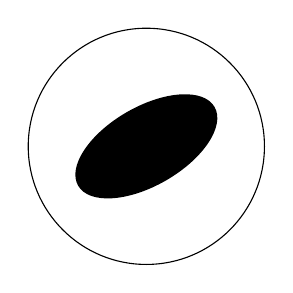
\begin{tikzpicture}
\draw (1,0) circle [radius=1.5];
\fill (1,0) circle [x radius=1cm, y radius=5mm, rotate=30];
\end{tikzpicture}

% 159
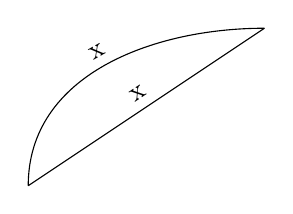
\begin{tikzpicture}
\draw (0,0) to [edge node={node [sloped,above] {x}}] (3,2);
\draw (0,0) to [out=90,in=180,
edge node={node [sloped,above] {x}}] (3,2);
\end{tikzpicture}

% 175
\tikz \shadedraw [shading=axis] (0,0) rectangle (1,1);
\tikz \shadedraw [shading=radial] (0,0) rectangle (1,1);
\tikz \shadedraw [shading=ball] (0,0) circle (.5cm);

% 234
\begin{tikzpicture}[level distance=8mm]
\node (root) {root}
child { node (a) {a} }
child { node (b) {b}
child { node (d) {d} }
child { node (e) {e} } }
child { node (c) {c} };
\begin{pgfonlayer}{background}
\node[fill=red!20,inner sep=0pt,ellipse,fit=(root) (b) (d) (e)] {};
\node[fill=blue!20,inner sep=0pt,ellipse,fit=(b) (c) (e)] {};
\end{pgfonlayer}
\end{tikzpicture}

% 238
\tikz [allow upside down]
\draw (0,0) .. controls +(up:2cm) and +(left:2cm) .. (1,3)
node foreach \p in {0,0.25,...,1} [sloped,above,pos=\p]{\p};

% 246
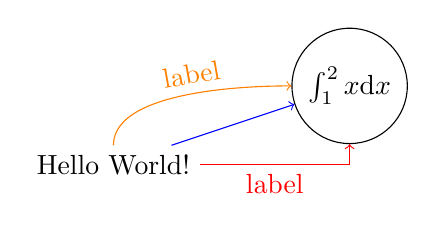
\begin{tikzpicture}
\path (0,0) node
 (x) {Hello World!}
(3,1) node[circle,draw](y) {$\int_1^2 x \mathrm d x$};
\draw[->,blue]
 (x) -- (y);
\draw[->,red]
 (x) -| node[near start,below] {label} (y);
\draw[->,orange] (x) .. controls +(up:1cm) and +(left:1cm) .. 
node[above,sloped] {label} (y);
\end{tikzpicture}

% % 249
% \begin{tikzpicture}[remember picture]
% \node (c) [circle,draw] {Big circle};
% \draw [overlay,->,very thick,red,opacity=.5]
% (c) to[bend left] (n1) (n1) -| (n2);
% \end{tikzpicture}

% % 346
% \tikzfading[name=fade inside,
% inner color=transparent!80,
% outer color=transparent!30]
% \begin{tikzpicture}
% % Checker board
% \fill [black!20] (0,0) rectangle (4,4);
% \path [pattern=checkerboard,pattern color=black!30] (0,0) rectangle (4,4);
% \shade [ball color=red] (3,3) circle (0.8);
% \shade [ball color=white,path fading=fade inside] (2,2) circle (1.8);
% \end{tikzpicture}

% 603
\begin{tikzpicture}
a big \draw [help lines] grid (3,2);
 \draw [red, dashed]
[postaction={decoration={text along path, text={a big juicy apple},
text align={align=right}}, decorate}]
 (0,0) .. controls (0,2) and (3,2) .. (3,0);
\end{tikzpicture}

% 754
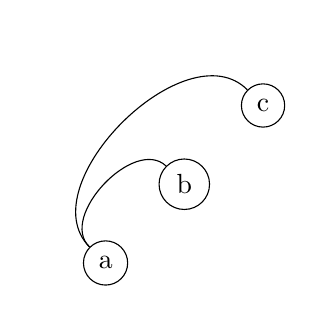
\begin{tikzpicture}[out=90,in=90,relative]
\node [circle,draw] (a) at (0,0) {a};
\node [circle,draw] (b) at (1,1) {b};
\node [circle,draw] (c) at (2,2) {c};
\path (a) edge (b)
edge (c);
\end{tikzpicture}

% % 841
% \tikz \datavisualization [
% school book axes,
% x axis={label=£x£},
% visualize as smooth line/.list={log, lin, squared, exp},
% every data set label/.append style={text colored},
% log= {pin in data={text’=£\log x£, when=y is -1}},
% lin= {pin in data={text=£x/2£, when=x is 2,
%       pin length=1ex}},
% squared={pin in data={text=£x^2£, when=x is 1.1,
%          pin angle=230}},
% exp= {label in data={text=£e^x£, when=x is -2}},
% style sheet=vary hue]
% data group {function classes};

\end{comment}

%--------------------------------------------------------------------
% Vecchia versione
%--------------------------------------------------------------------

\begin{comment}

\chapter{Funzioni}

Riprendiamo ora il concetto di funzione, precedentemente studiato nel 
capitolo 
12 del secondo volume, approfondendone alcuni aspetti che ci saranno utili 
nel 
proseguo del nostro percorso.

\section{Definizione di funzione}
%label{}
\begin{definizione}
  Dati due insiemi $A$ e $B$ non vuoti definiti in $\mathbb{R}$ è detta 
$f$, \textsc{funzione reale di variabile reale}, una qualsiasi legge, 
applicazione o corrispondenza che associa a ogni elemento di $A$ uno e un 
solo elemento di $B$.
\end{definizione}

\begin{figure}[htpb!]
  \centering
  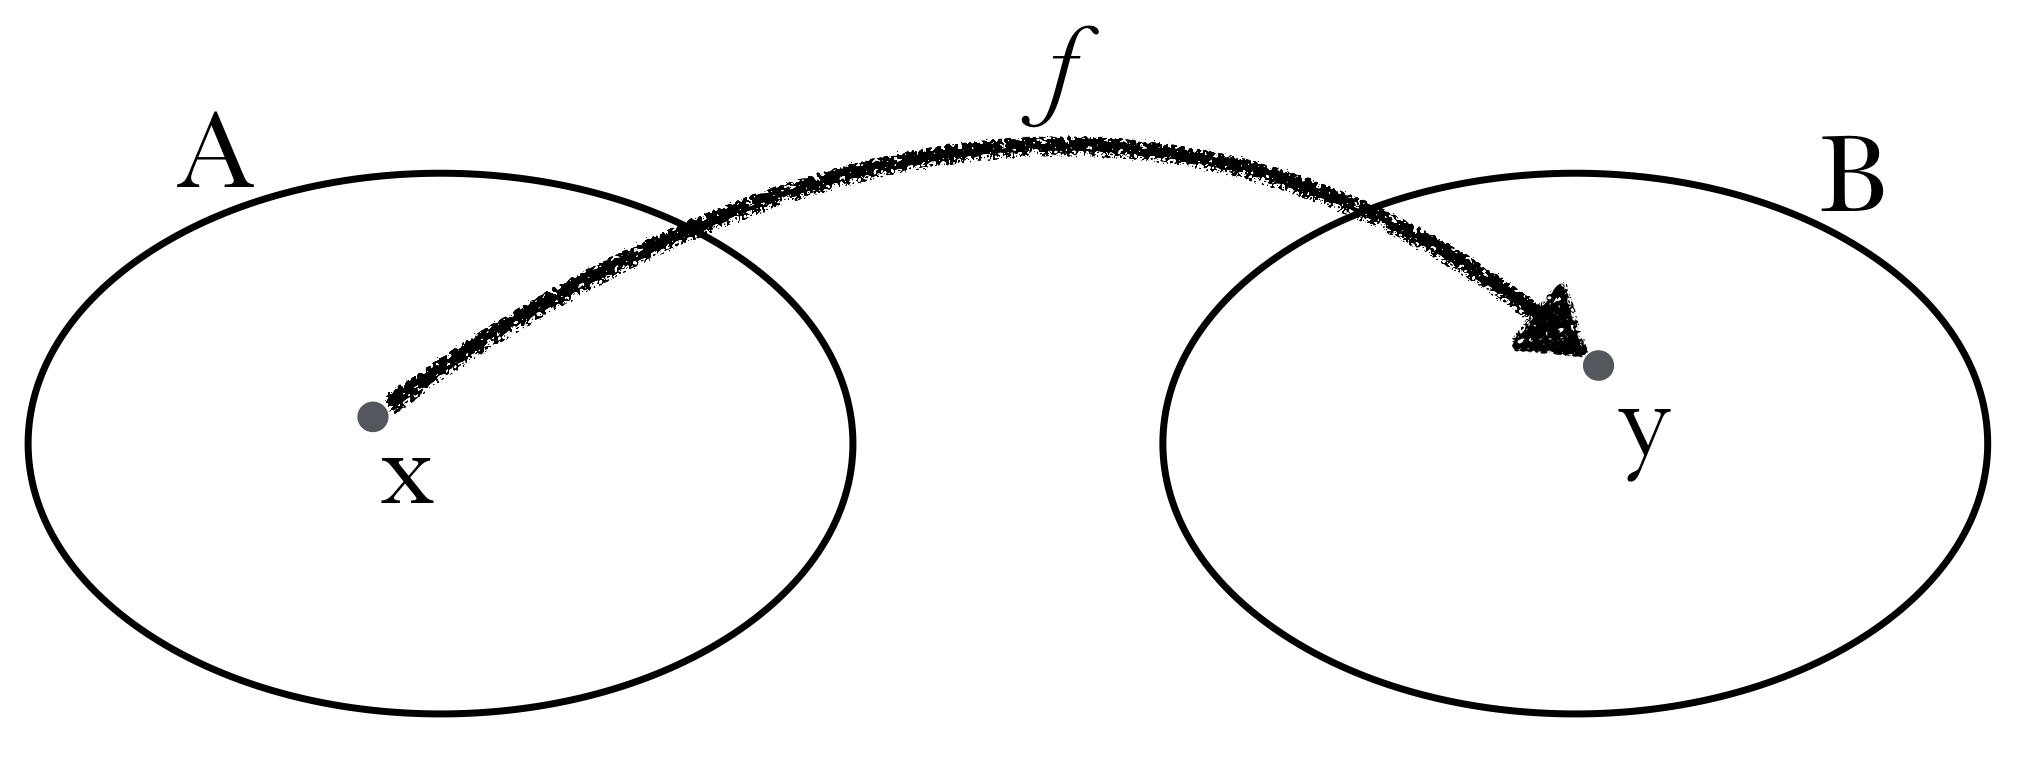
\includegraphics[width=0.55\textwidth]{img/1_funz.png}
  %%\caption{}
  %%\label{fig:1_1}
\end{figure}

Una funzione viene indicata:\\

$f: A\to B  $  tra insiemi   $f: x\mapsto y$   tra elementi  con $x\in A 
$  e $y\in B$\\

Dobbiamo pensare che $x$ mediante la corrispondenza $f$ diventa $y$, 
l'elemento $y$ è dunque l'\textsc{immagine} di $x$ mediante la 
trasformazione 
$f$; altrettanto e viceversa possiamo chiamare $x$ \textsc{controimmagine} 
di 
$y$.\\

L'elemento $x$ viene dunque proiettato mediante una sua trasformazione che 
chiamiamo $f$ nell'elemento $y$ di $B$, $y$ risulta così dipendente da $x$ 
perché determinata proprio in funzione di $x$, variabile indipendente.\\

L'immagine $y$ risulta propriamente in funzione di $x$ e possiamo scrivere 
$f(x)=y$ e la precedente espressione tra elementi diventa $f: x\mapsto 
f(x)=y$.\\

Definiamo $D$ \textsc{dominio} l'insieme $A$ delle $x$ e $C$ 
\textsc{codominio} il sottoinsieme di $B$ di tutte le immagini di $x$, cioè 
di tutte e sole le $y$ generate dalla trasformazione $f$.\\

\begin{figure}[htpb!]
  \centering
  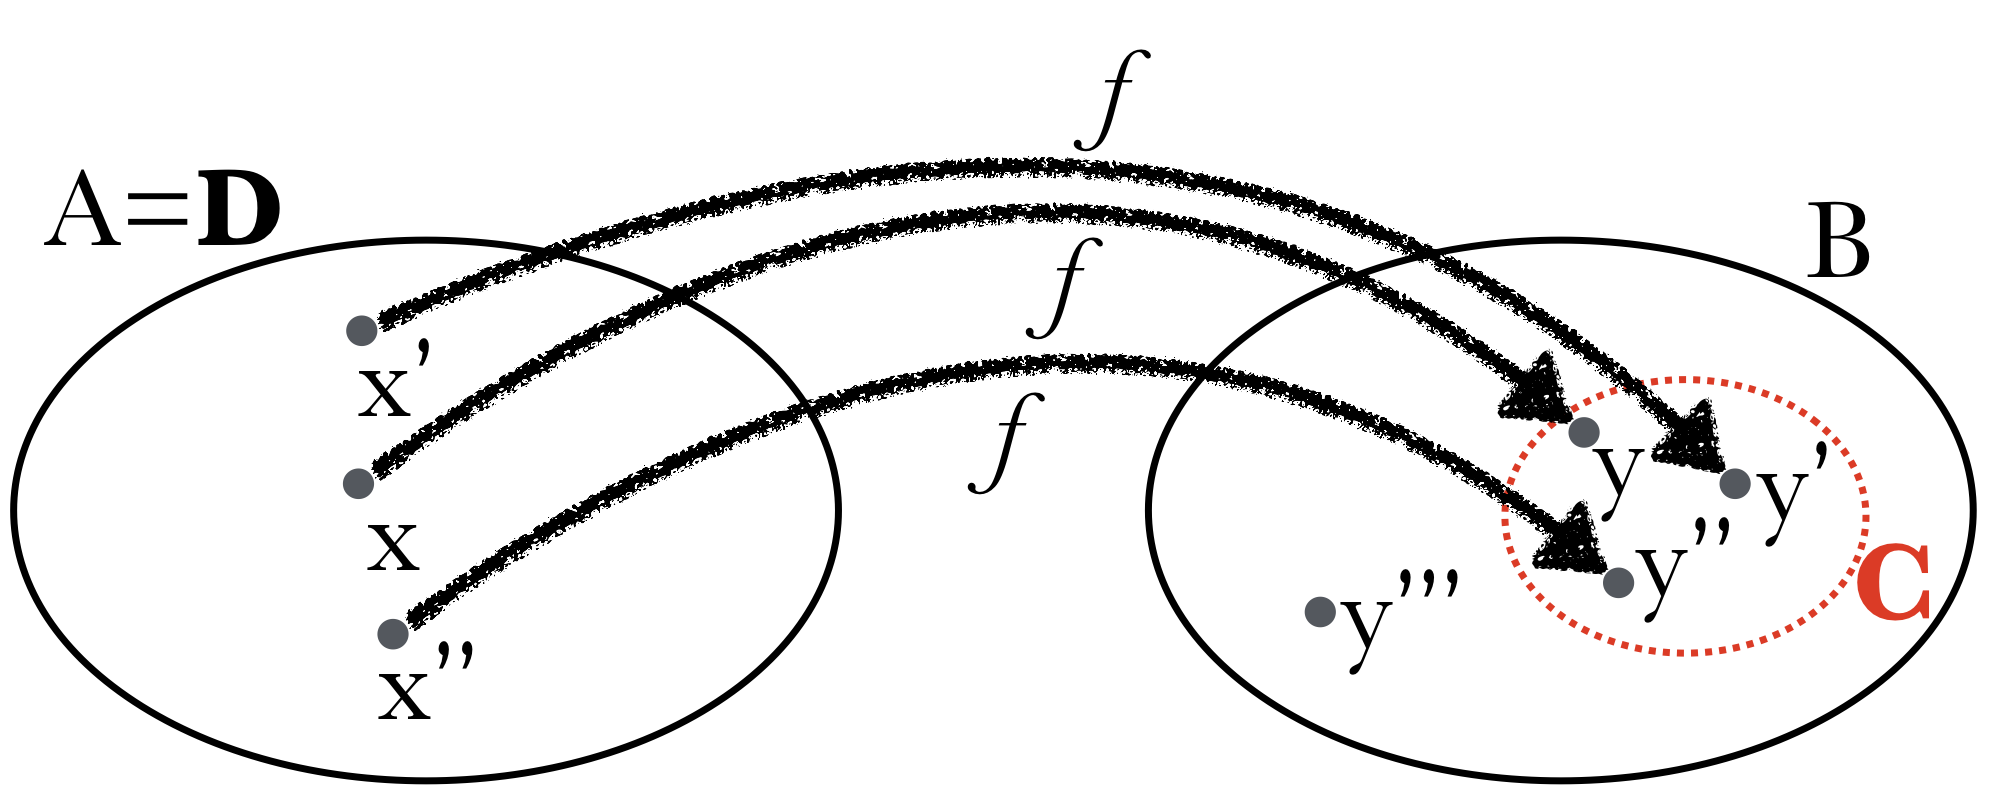
\includegraphics[width=0.55\textwidth]{img/2_funz.png}
  %\caption{}
  %\label{fig:1_2}
\end{figure}
%
Notiamo, nella figura precedente che mentre il dominio coincide con 
l'insieme 
di partenza il codominio è un sottoinsieme dell'insieme di arrivo.\\

%
%
%
\begin{esempio}
  Visualizziamo dominio e codominio della funzione $f(x)=x^2$
  \begin{figure}[htpb!]
  \centering
  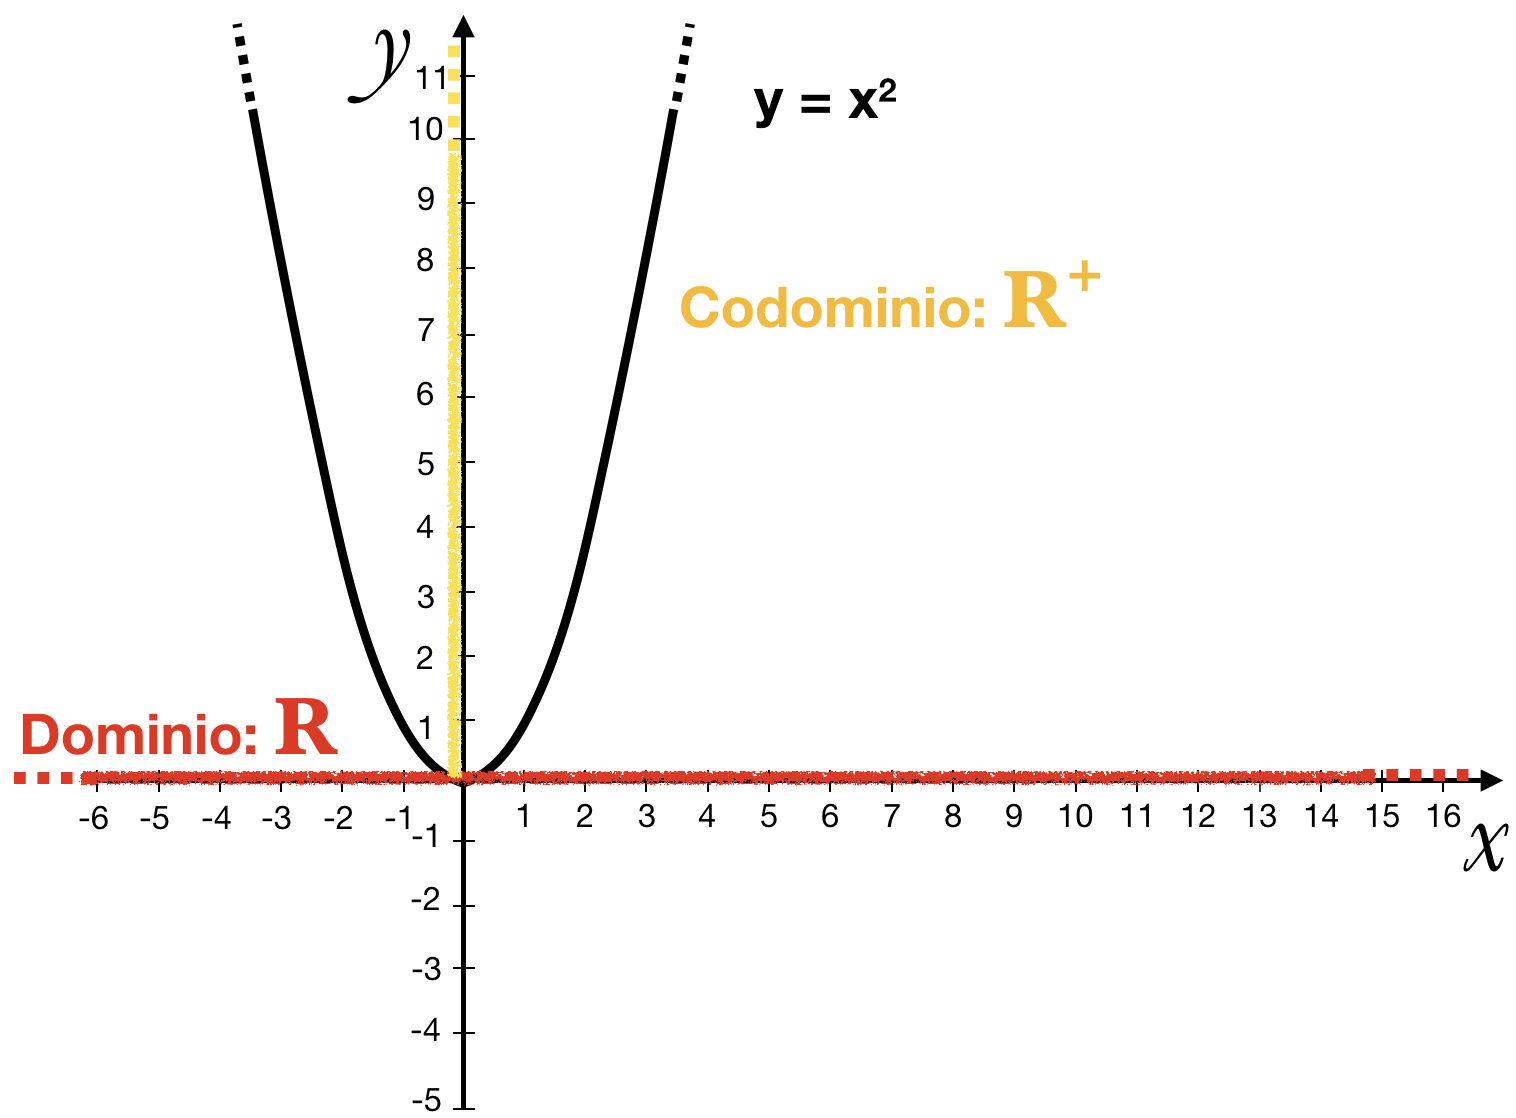
\includegraphics[width=0.4\textwidth]{img/2a_funz.png}
  %\caption{}
  %\label{fig:1_2}
  \end{figure}
\end{esempio}

\begin{esempio}
  Visualizziamo dominio e codominio della funzione $f(x)=\log{x}$
  \begin{figure}[htpb!]
  \centering
  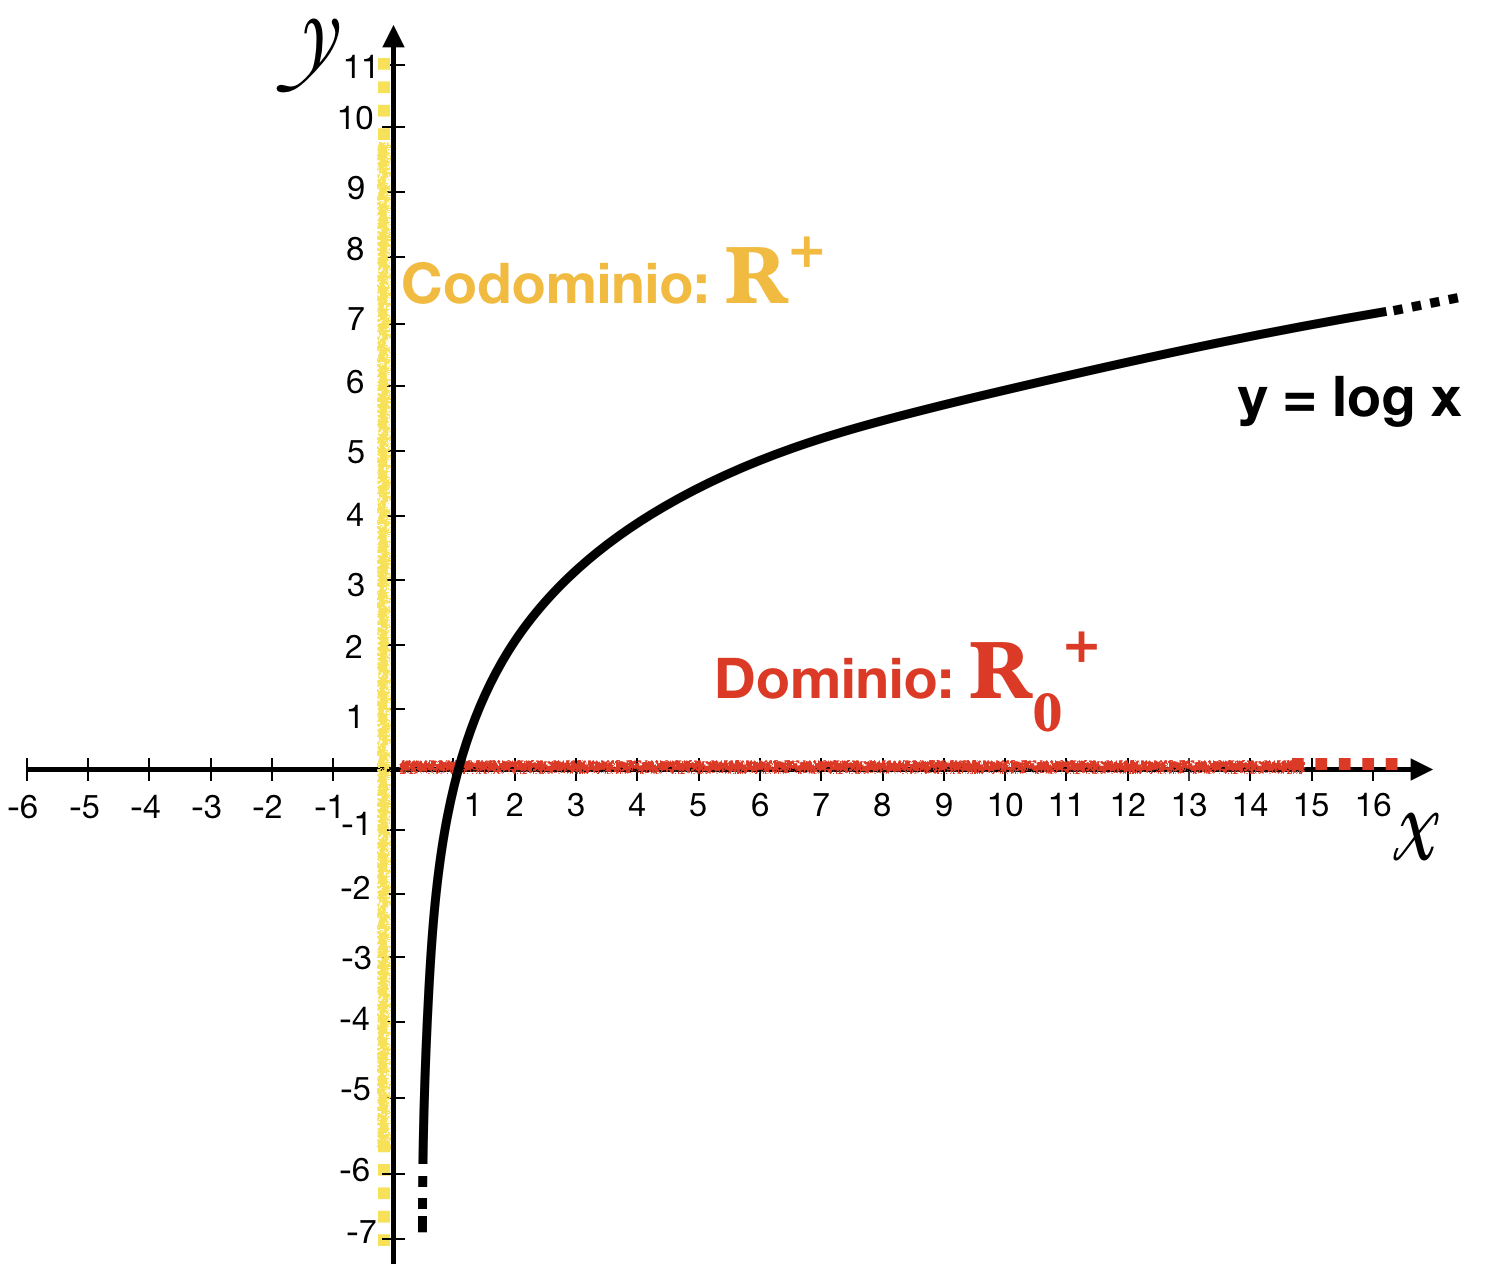
\includegraphics[width=0.4\textwidth]{img/2b_funz.png}
  %\caption{}
  %\label{fig:1_2}
  \end{figure}
\end{esempio}

\begin{esempio}
  Visualizziamo dominio e codominio della funzione $f(x)=\frac{9}{x}$
  \begin{figure}[htpb!]
  \centering
  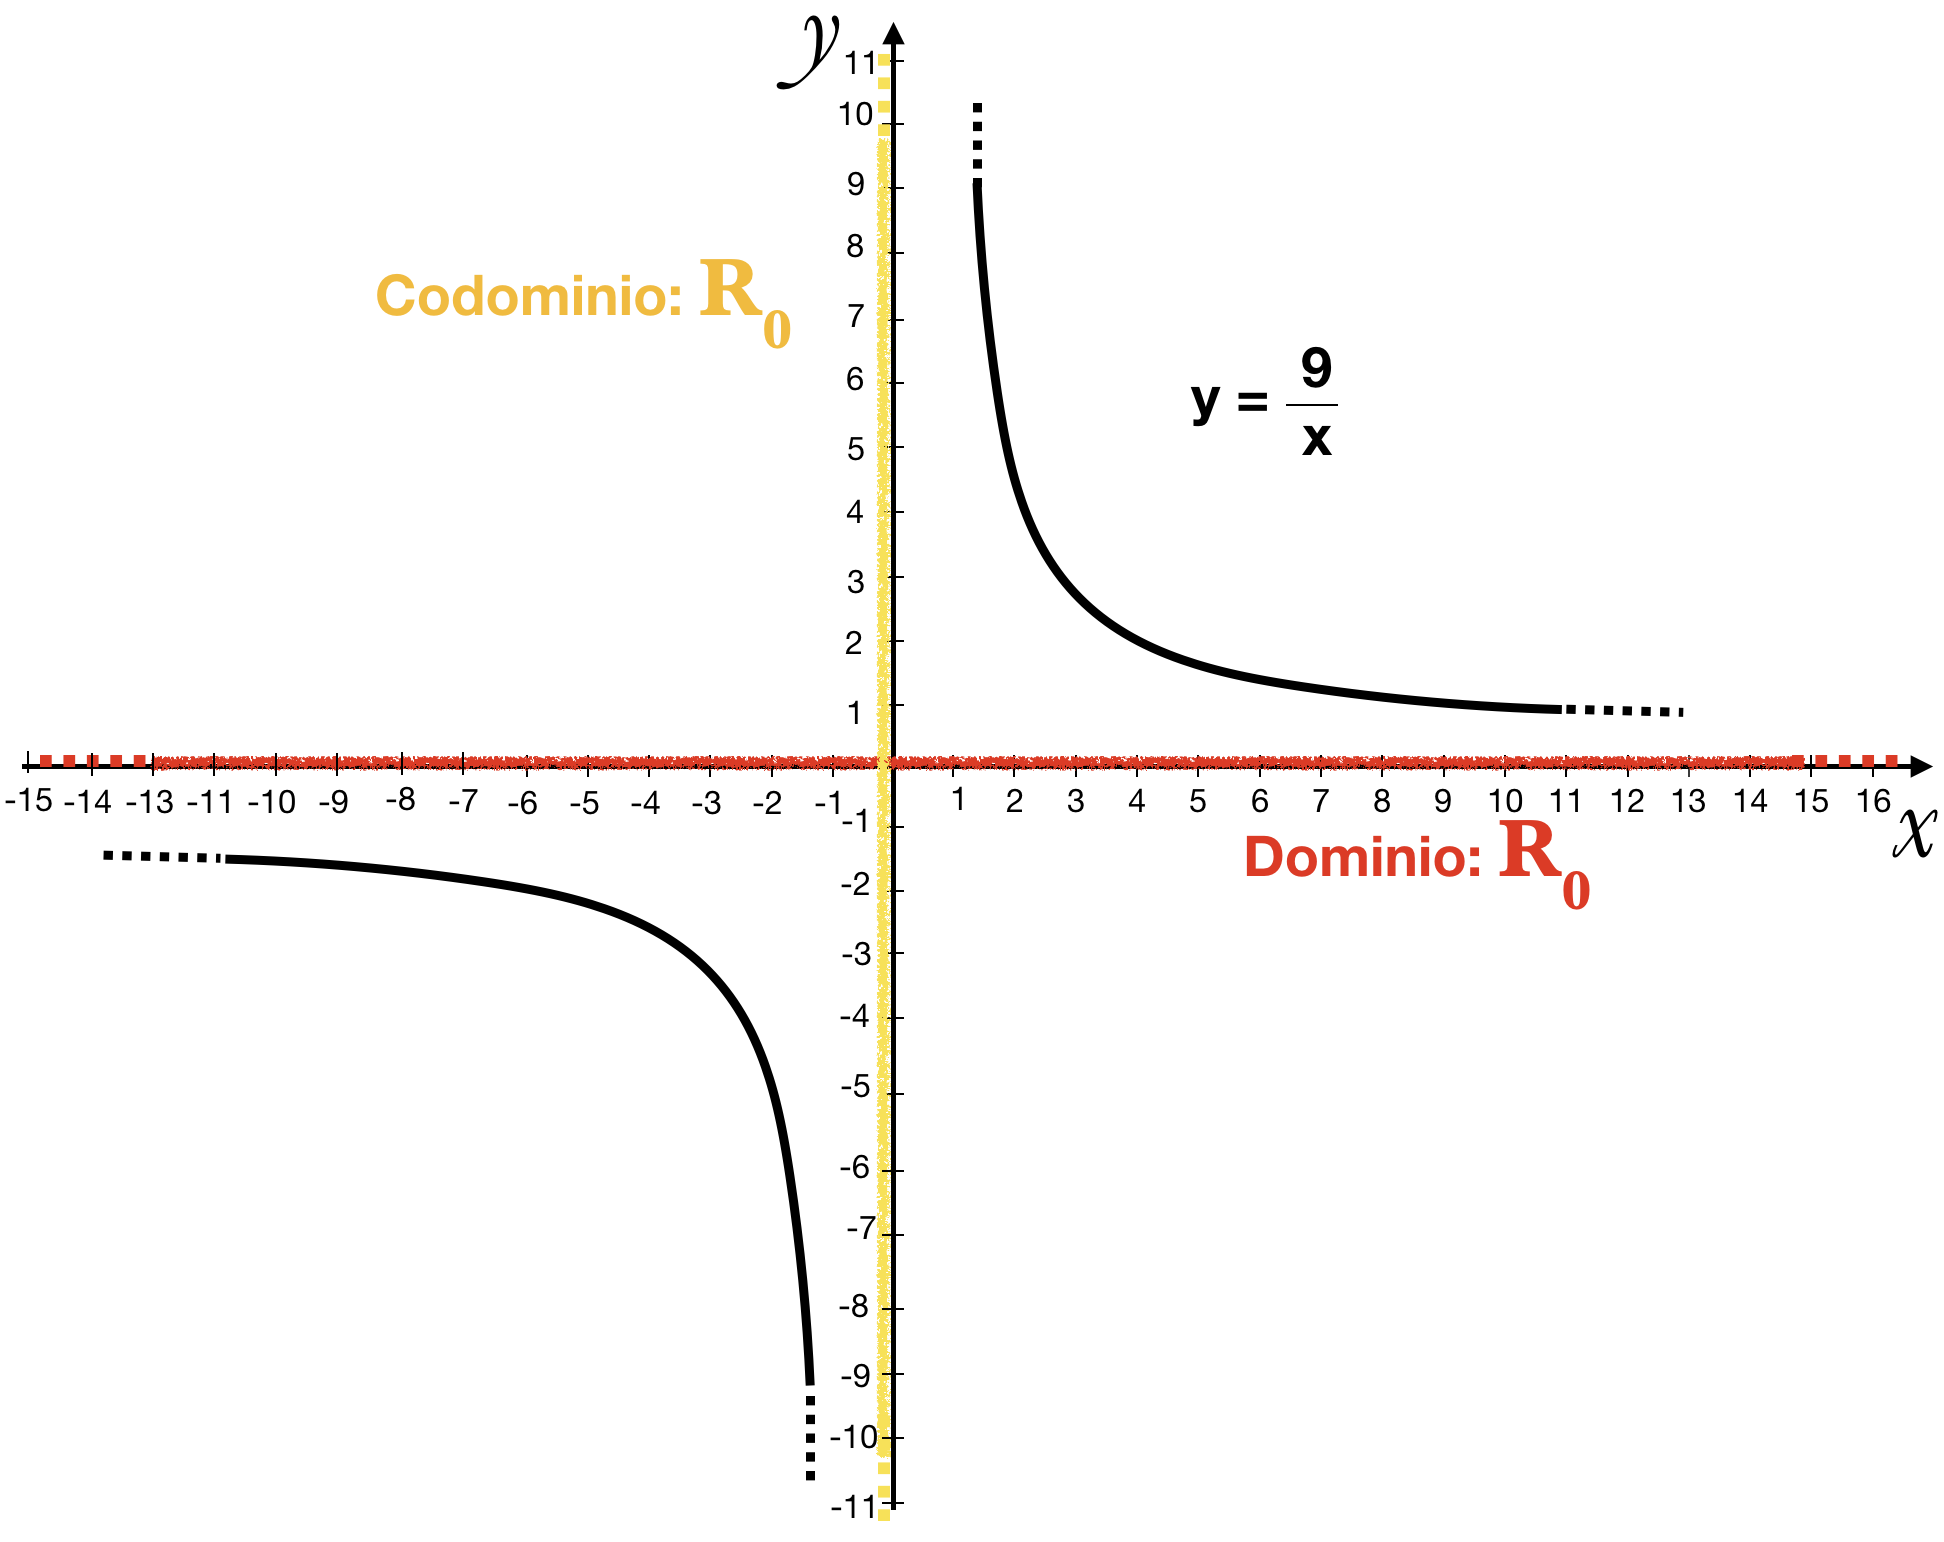
\includegraphics[width=0.55\textwidth]{img/2c_funz.png}
  %\caption{}
  %\label{fig:1_2}
  \end{figure}
\end{esempio}

\newpage 
Per calcolare il dominio delle funzioni, vediamo una tabella riassuntiva 
dei 
possibili casi.\\

%%%%%%%%%%%%%%TABELLA DOMINIO FUNZIONI%%%%%%%%%%%%
\begin{table}

\raggedleft
%   \begin{tabularx}{1,2\textwidth}{XXX}
  \begin{tabularx}{\textwidth}{XXX}
  \toprule
  Funzione & Dominio  & Esempio \\
  \midrule
  
  \textbf{Funzioni razionali intere} 
\newline$y=a_0x^n+a_1x^{n-1}+\dots+a_n$ 
  & $\,$ \newline $D=\mathbb{R}$ 
  & $\,$ \newline $y=x^3-x^2+2x+1$ \newline $D=\mathbb{R}$ \\
  \midrule

  \textbf{Funzioni razionali fratte} \newline 
$y=\frac{A(x)}{B(x)}$ \newline con $A(x)$ e $B(x)$ polinomi 
  & $\mathbb{R}$ esclusi i valori che annullano $B(x)$, cioè 
\newline $B(x)\neq 0$
  & $\,$ \newline$y=\frac{3+x^2}{x-5}$\newline $D= 
\mathbb{R}-\{5\}$ \\
  \midrule

  \textbf{Funzioni irrazionali} \newline $y=\sqrt[n]{f(x)}$ 
\newline con $n\in\mathbb{N},\,n>1$ 
  & $\,$ \newline Se $n$ è dispari il $D$ è il $D$ di $f(x)$ 
\newline \newline Se $n$ è pari, \newline$D=\{x\in\mathbb{R}\vert 
f(x)\geq0\}$
  & $\,$ \newline $y=\sqrt[3]{x^2-9}$\newline $D=\mathbb{R}$ 
\newline \newline $y=\sqrt{x^2-1}$\newline $D=x^2\geq1=$\newline 
$=x\leq-1\lor x\geq1$ \\
  \midrule
  
  \textbf{Funzioni logaritmiche} \newline $y=\log_af(x)$ 
\newline con $a>0,\,a\neq1$ \newline \newline $y=\log_{g(x)}(f(x))$ 
  & $\,$ \newline $D=\{x\in\mathbb{R}\vert f(x)>0\}$\newline 
\newline \newline$D=\{x\in\mathbb{R}\vert f(x)>0\land$\newline$\land 
g(x)>0\land g(x)\neq1\}$
  & $\,$ \newline $y=\log(x+1)$\newline $D=x>-1$\\
  \midrule
  
   \textbf{Funzioni esponenziali} \newline $y=a^{f(x)}$ 
\newline con $a>0,\,a\neq1$ \newline\newline  $y={f(x)}^{g(x)}$ 
  & $\,$ \newline $D$ di $f(x)$ \newline \newline \newline 
$D=\{x\in\mathbb{R}\vert f(x)>0\}\land$ $D$ di $g(x)$
  &  $\,$ \newline$y=3^{2x}$\newline $D= \mathbb{R}$ \newline  
\newline$y=e^{\frac{1}{x+1}}$ \newline $D=\mathbb{R}-\{-1\}$ \\
  \midrule
  
  \textbf{Funzioni potenza} \newline $y=f(x)^a$ \newline con 
$a\in\mathbb{R},\,a\neq0$ \newline \newline$a$ intero positivo \newline 
\newline $a$ intero negativo \newline  \newline $a$ razionale \newline  
\newline$a$ irrazionale positivo \newline \newline $a$ irrazionale negativo 
  & $\,$  \newline  \newline  \newline  \newline  $D$ di $f(x)$ 
\newline  \newline $D$ di $f(x)$ con $f(x)\neq0$\newline \newline $D$ di 
$f(x)$ razionale \newline \newline $D=\{x\in\mathbb{R}\vert 
f(x)\geq0\}$\newline \newline $D=\{x\in\mathbb{R}\vert f(x)>0\}$
  & $\,$  \newline  \newline  \newline  \newline $y=(x-1)^2$ 
$D=\mathbb{R}$ \newline \newline $y=(x-1)^{-2}$ $D=x\neq1$ \newline 
\newline 
$y=(x-1)^{1/2}=\sqrt{x-1}$ $D=x\geq1$ \newline $y=(x-1)^{\pi}$ $D=x\geq1$ 
\newline \newline $y=(x-1)^{-\pi}$ $D=x>1$\\
  \midrule

  \textbf{Funzioni goniometriche} \newline $y=\sin{x}$, 
$y=\cos{x}$ \newline \newline $y=\tan x$, $y=\sec x$ \newline  \newline 
$y=\cot x$, $y=\csc x$ 
  & $\,$ \newline $D=\mathbb{R}$ \newline  \newline 
$D=\mathbb{R} -\bigl\{\frac{\pi}{2}+k\pi \bigr\}$\newline \newline 
$D=\mathbb{R} -\{k\pi\}$
  &  \\
  \midrule
  
\end{tabularx}
\end{table}

\begin{table}   

\raggedleft   
\begin{tabularx}{\textwidth}{XXX}
  \midrule

  \textbf{Funzioni goniometriche inverse} \newline 
$y=\arcsin{x}$, $y=\arccos{x}$ \newline \newline $y=\arctan x$, 
$y=\text{arccot}\,x$
  & $\,$ \newline \newline $D=[-1,1]$ \newline  \newline 
$D=\mathbb{R}$
  &  \\
  \midrule

  \textbf{Funzioni goniometriche composte} \newline 
$y=\sin[f(x)]$, $y=\cos [f(x)]$ \newline \newline $y=\tan [f(x)]$ \newline 
\newline \newline $y=\cot [f(x)]$ \newline  \newline $y=\arcsin[f(x)]$, 
\newline $y=\arccos [f(x)]$ \newline \newline $y=\arctan [f(x)]$
  & $\,$ \newline \newline $D$ di $f(x)$ \newline  \newline 
$D=\bigl\{x\in\mathbb{R}\vert f(x)\neq\frac{\pi}{2}+\newline+k\pi 
\bigr\}$\newline \newline $D=\{x\in\mathbb{R}\vert f(x)\neq k\pi\}$ 
\newline 
\newline $D=\{x\in\mathbb{R}\vert -1\leq f(x)\leq\newline\leq1\}$ \newline 
\newline $D$ di $f(x)$
  & $\,$ \newline \newline \newline $y=\tan[2x-1]$ \newline 
$2x-1\neq \frac{\pi}{2}+k\pi$ \newline$D=x\neq\frac{\pi+1+k\pi}{2}$  
\newline 
\newline \newline  $y=\arcsin[x-1]$ \newline $-1\leq x-1\leq1$\newline 
$0\leq 
x\leq2$\newline \newline$y=\arctan [\frac{x+2}{x+3}]$ \newline 
$D=\mathbb{R}-\{-3\}$
 \\

  \bottomrule
\end{tabularx}
\end{table}
\newpage

\section{La rappresentazione di una funzione}
%label{}
Una funzione può essere rappresentata in diversi modi, i principali sono:
\begin{itemize}
  \item \textsc{Rappresentazione tabulare}\\
Le funzioni empiriche vengono ricostruite con una tabella in cui ad ogni 
$y$ 
corrisponde un certo $x$. Ad esempio pensiamo ad una tabella che dà la 
temperatura ora per ora in un certo luogo.
%
  \item \textsc{Rappresentazione analitica}\\
La funzione è espressa mediante un insieme di operazioni matematiche che 
applicate in un certo ordine ad $x$ restituiscono un corrispondente valore 
di 
$y$. Esempi ne sono $y=\log{(x+2)}$, $y=2x^3+3$ o $y=\sin{x}+2^x$, cioè le 
espressioni, scritte in linguaggio matematico, che siamo abituati a 
trattare.
%
  \item \textsc{Rappresentazione grafica}\\
La funzione è rappresentata come una corrispondenza $x-$y su un grafico 
cartesiano; in particolare, ricordiamo che: il grafico di una funzione $f 
:A\to B$ è l'insieme di tutte le coppie ordinate $(x;y)$ che si ottengono 
prendendo un valore $x$ in $A$ e trovando il corrispondente valore $y=f(x)$ 
in $B$. Ogni coppia ordinata rappresenta un punto nel piano cartesiano 
$\mathbb{R}^2$.
\end{itemize}

\section{Le proprietà di una funzione}
%label{}
Una funzione, a seconda, del modo in cui gli elementi del dominio 
corrispondono agli elementi del codominio si può definire 
\textsc{iniettiva}, 
\textsc{suriettiva} e \textsc{biiettiva} (o \textsc{biunivoca}).\\

\begin{definizione}
Una funzione da $A$ a $B$ si dice \textsc{iniettiva} se ogni elemento di 
$B$ 
è immagine di \underline{al più} un elemento di $A$;\\


$f : A\to B$ è iniettiva se  $\forall x_1,\,x_2\in A ,\,x_1\neq 
x_2\Rightarrow f(x_1 )\neq f(x_2)$
\end{definizione}

\begin{figure}[htpb!]
  \centering
  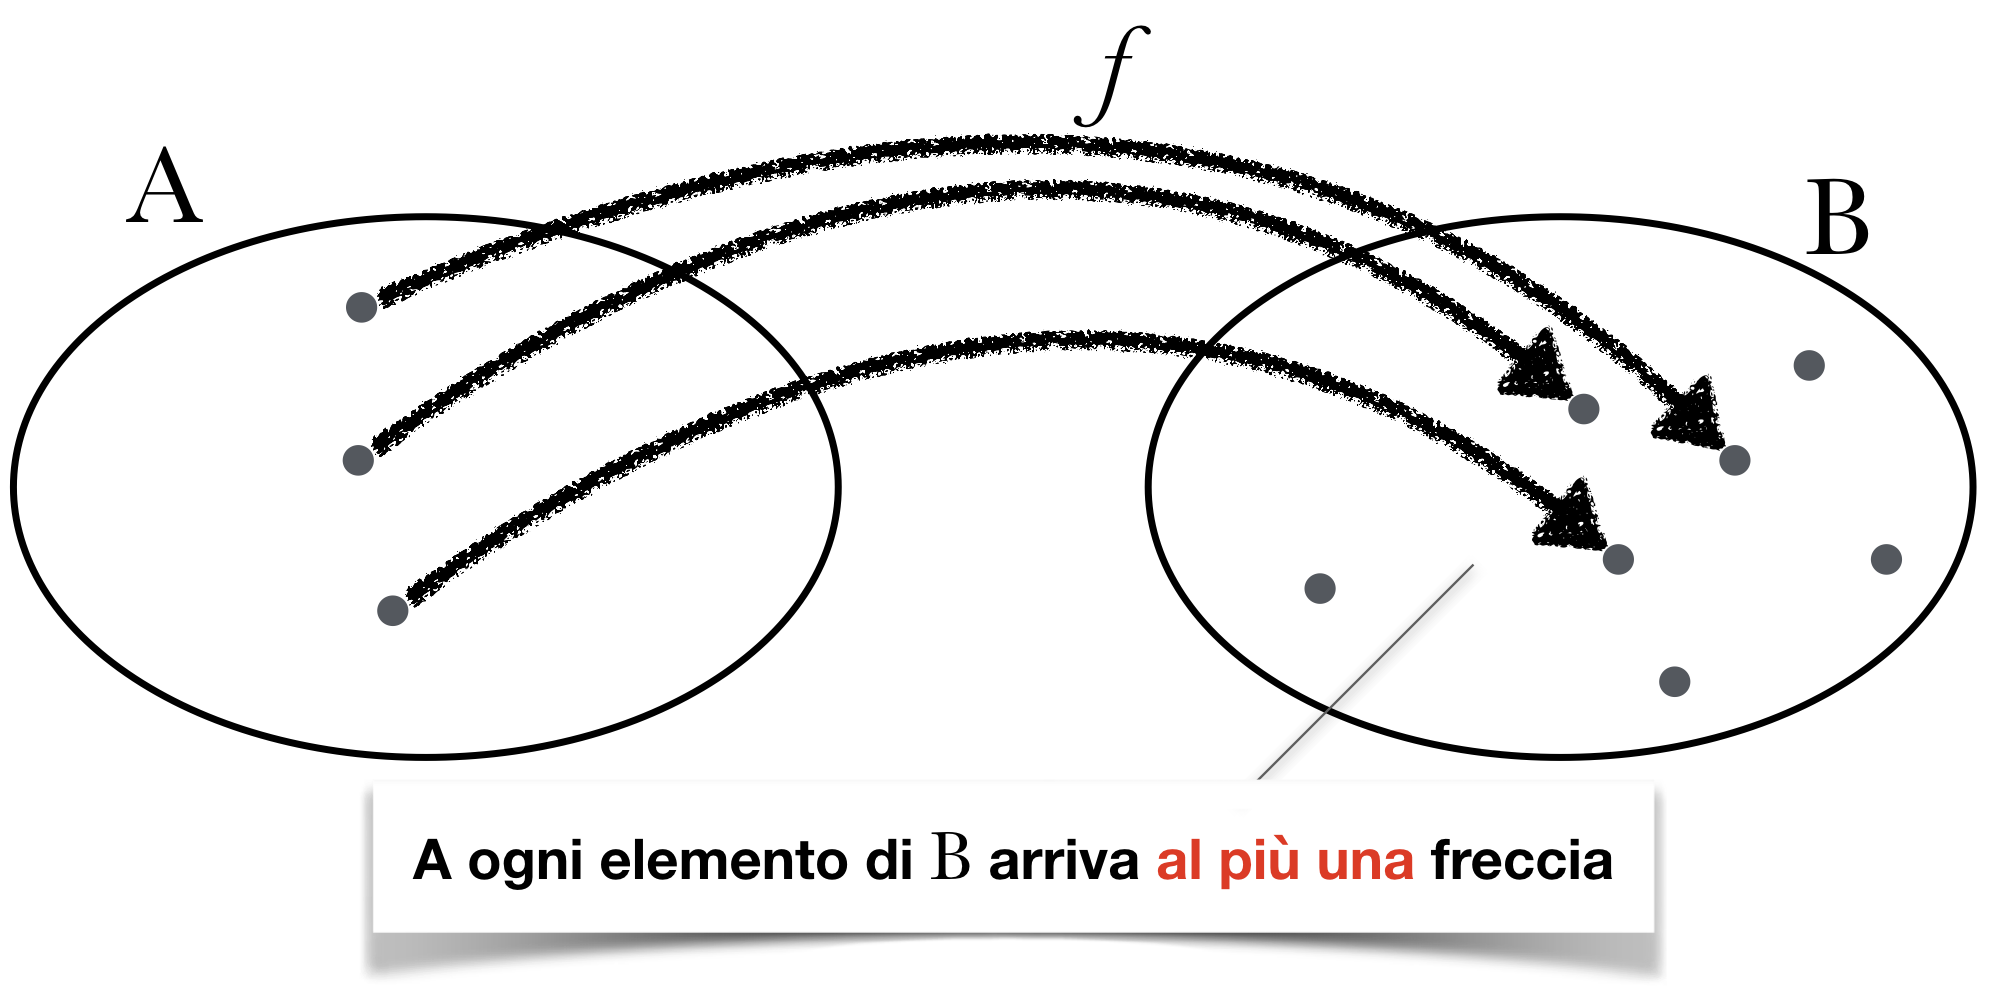
\includegraphics[width=0.55\textwidth]{img/3_funz.png}
  %\caption{}
  %\label{fig:1_2}
\end{figure}

\begin{definizione}
Una funzione da $A$ a $B$ si dice \textsc{suriettiva} quando ogni elemento 
di 
$B$ è immagine di \underline{almeno un} elemento di $A$;\\

$f: A\to B$ è suriettiva se $\forall y\in B, \exists x\in A \mid f(x)=y$
\end{definizione}

\begin{figure}[htpb!]
  \centering
  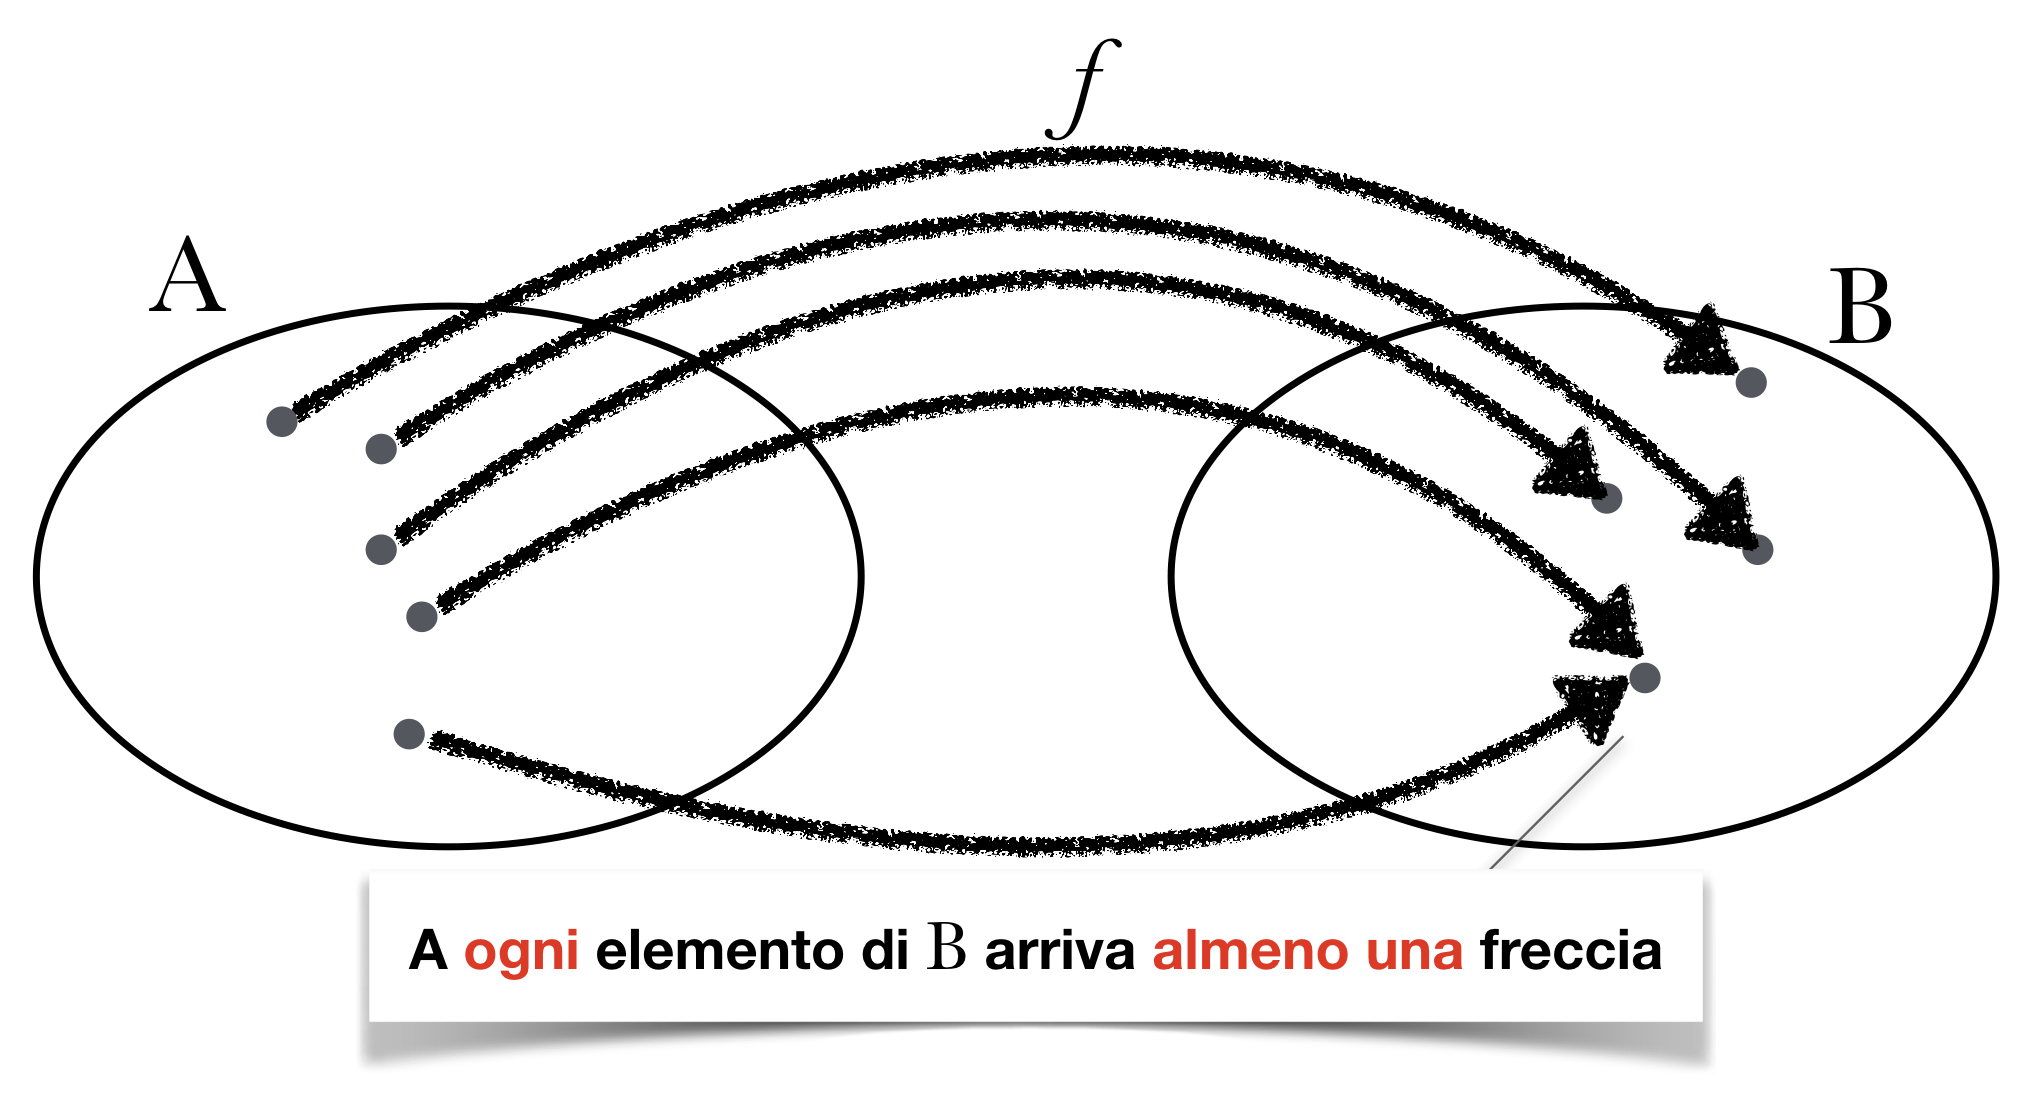
\includegraphics[width=0.55\textwidth]{img/4_funz.png}
  %\caption{}
  %\label{fig:1_2}
\end{figure}

Il fatto che una funzione sia o non sia suriettiva dipende da come si 
sceglie 
l'insieme di arrivo. Se lo si sceglie coincidente con il codominio la 
funzione è suriettiva.\\
%
\begin{definizione}
Una funzione da $A$ a $B$ è \textsc{biiettiva} (o \textsc{biunivoca}) 
quando 
è sia iniettiva sia suriettiva.\\
\end{definizione}

\begin{figure}[htpb!]
  \centering
  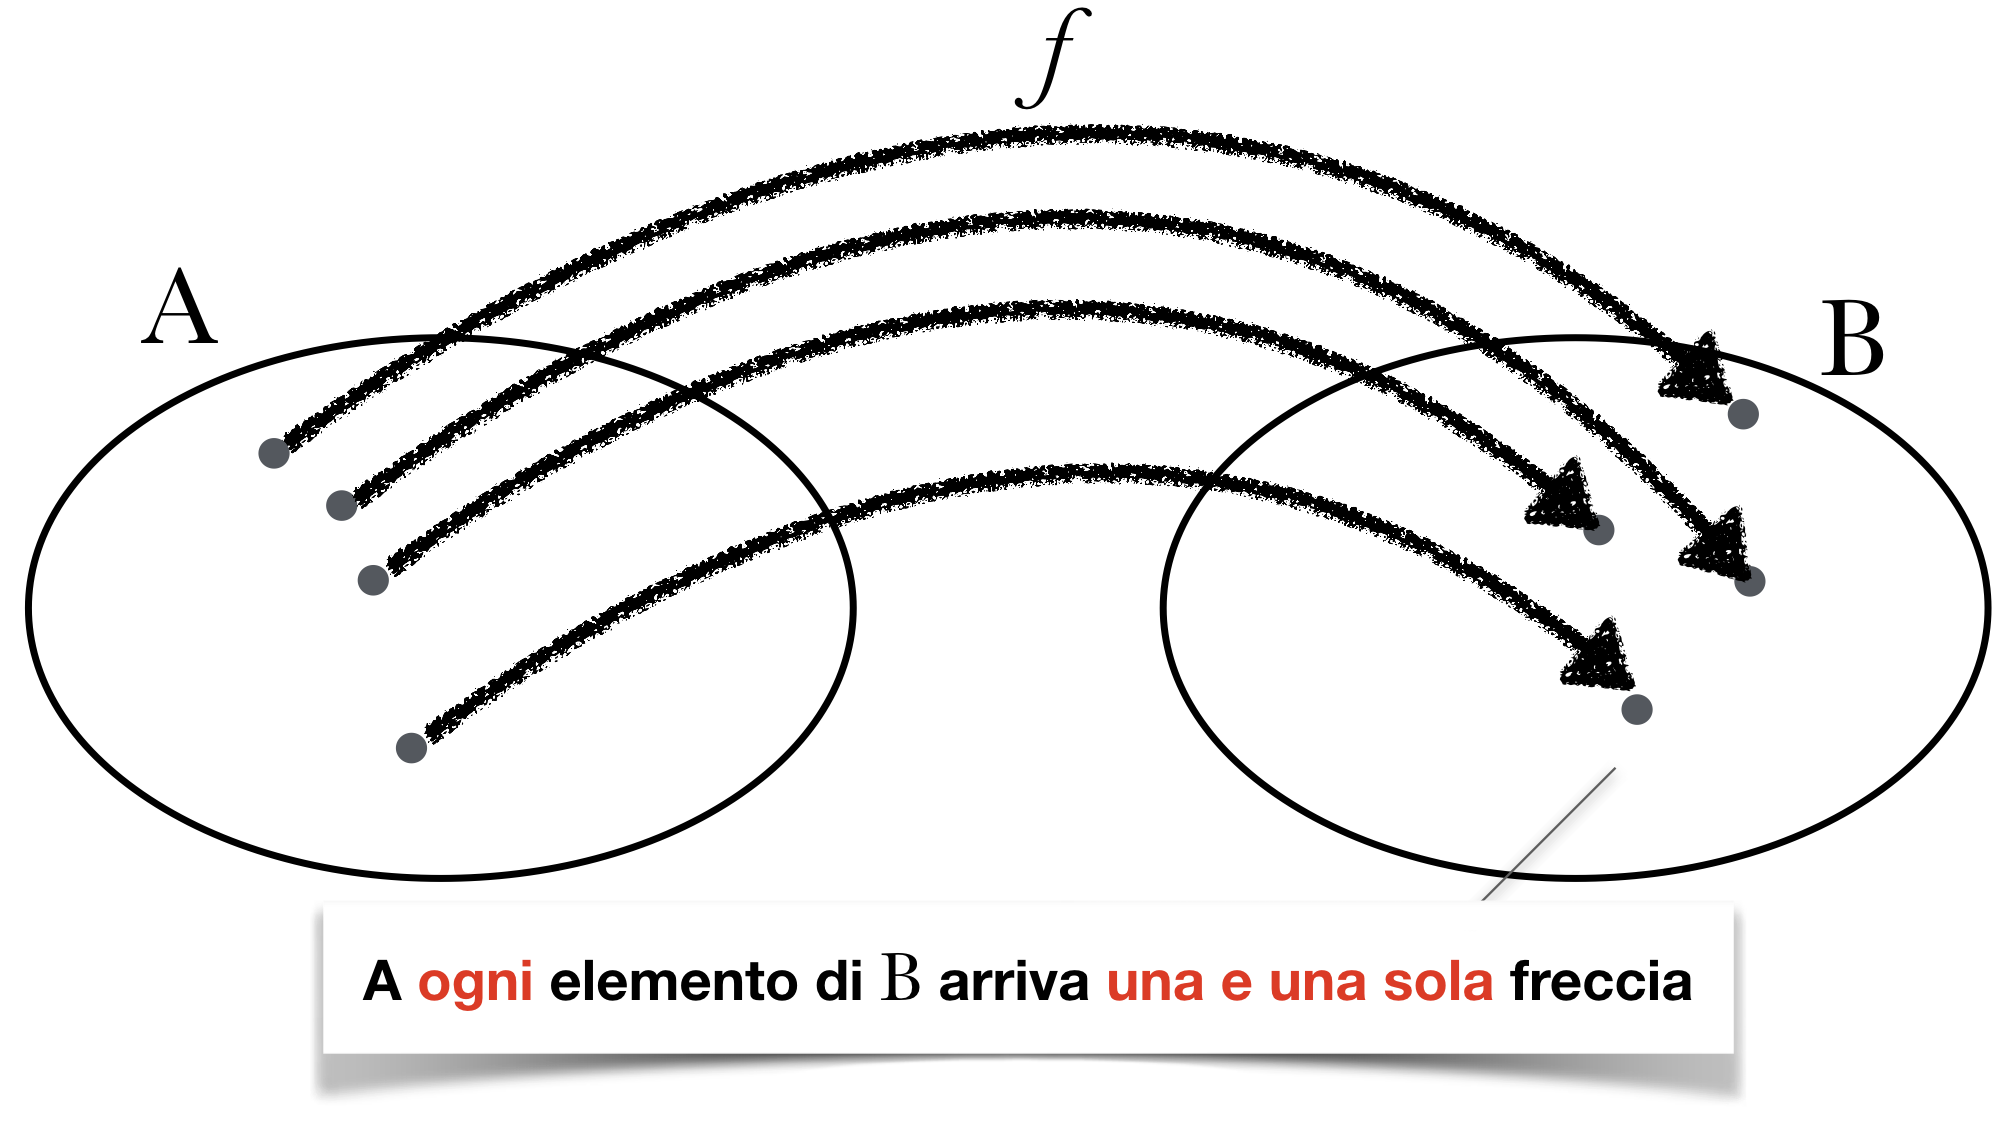
\includegraphics[width=0.55\textwidth]{img/5_funz.png}
  %\caption{}
  %\label{fig:1_2}
\end{figure}

\begin{esempio} Quando una funzione è biettiva?\\
Una funzione biiettiva è ad esempio una qualsiasi retta. Una retta è 
infatti 
sia iniettiva, che biettiva di dominio $\mathbb{R}$ e codominio 
$\mathbb{R}$.\\
\end{esempio}

Una funzione biiettiva viene anche detta biiezione o corrispondenza 
biunivoca 
fra gli insieme $A$ e $B$. Tale relazione tra insiemi è molto forte e 
specifica in quanto ad ogni elemento di $A$ viene associato un solo 
elemento 
di $B$ e, reciprocamente, ad ogni elemento di $B$ è associato un solo 
elemento di $A$, in una relazione uno a uno. Per tale ragione, la relazione 
tra i due insiemi viene indicata con una doppia freccia $A\leftrightarrow 
B$.
%
\section{Le caratteristiche di una funzione}
%label{}
Analizziamo ora le caratteristiche che può manifestare una funzione, 
qualità 
che può presentare il suo andamento e che possono contraddistinguerne la 
forma del grafico.

\subsection{Monotonia}
%label{}
La caratteristica della monotonia vuole evidenziare l'andamento 
\textsc{crescente} o \textsc{decrescente} di una funzione; la monotonia 
studia il comportamento della variabile dipendente $y$ all'aumentare della 
variabile indipendente $x$. All'aumentare dell'ascissa se aumenta anche 
l'ordinata diremo che la funzione cresce, se l'ordinata diminuisce diremo 
che 
la funzione decresce. Vediamo e puntualizziamo meglio.\\

\begin{definizione}
Una funzione $y=f(x)$ di dominio $D$, si dice \textsc{crescente in senso 
stretto} in un intervallo $I$, sottoinsieme di $D$, se\\

$\forall x_1,x_2\in I$  con $x_1<x_2 $ si ha $f(x_1)<f(x_2)$\\
\end{definizione}

\begin{figure}[htpb!]
  \centering
  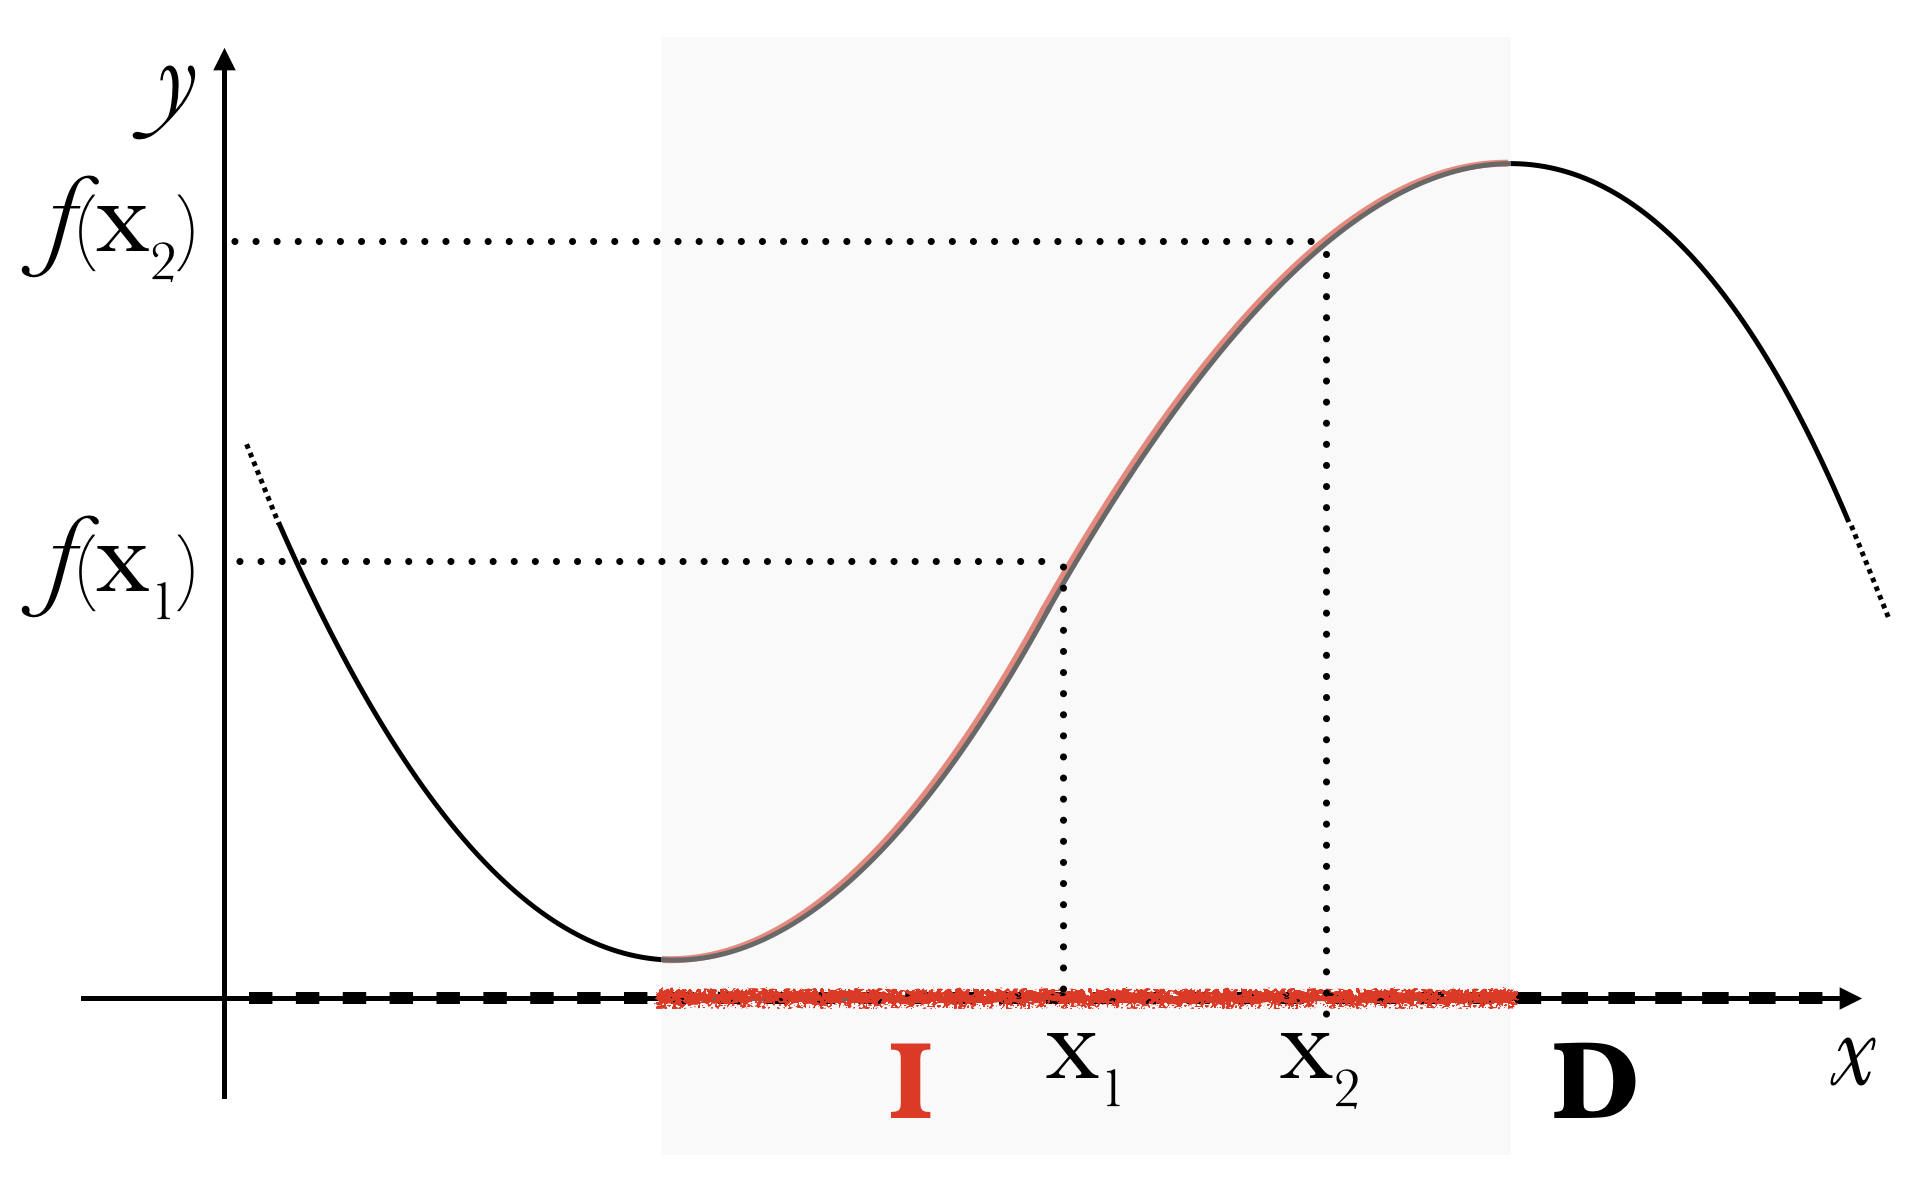
\includegraphics[width=0.55\textwidth]{img/funz_6.png}
  %\caption{}
  %\label{fig:1_2}
\end{figure}
%
\begin{definizione}
Una funzione è non decrescente o \textsc{crescente} in senso lato in un 
intervallo $I$, sottoinsieme di $D$, se\\

$\forall x_1,x_2\in I$  con $x_1<x_2 $ si ha $f(x_1)\leq f(x_2)$\\
%
\end{definizione}
%
%
%

\begin{definizione}
Una funzione $y=f(x)$ di dominio $D$, si dice \textsc{decrescente in senso 
stretto}, in un intervallo $I$, sottoinsieme di $D$, se\\

$\forall x_1,x_2\in I$  con $x_1<x_2 $ si ha $f(x_1)> f(x_2)$\\

\end{definizione}

\begin{figure}[htpb!]
  \centering
  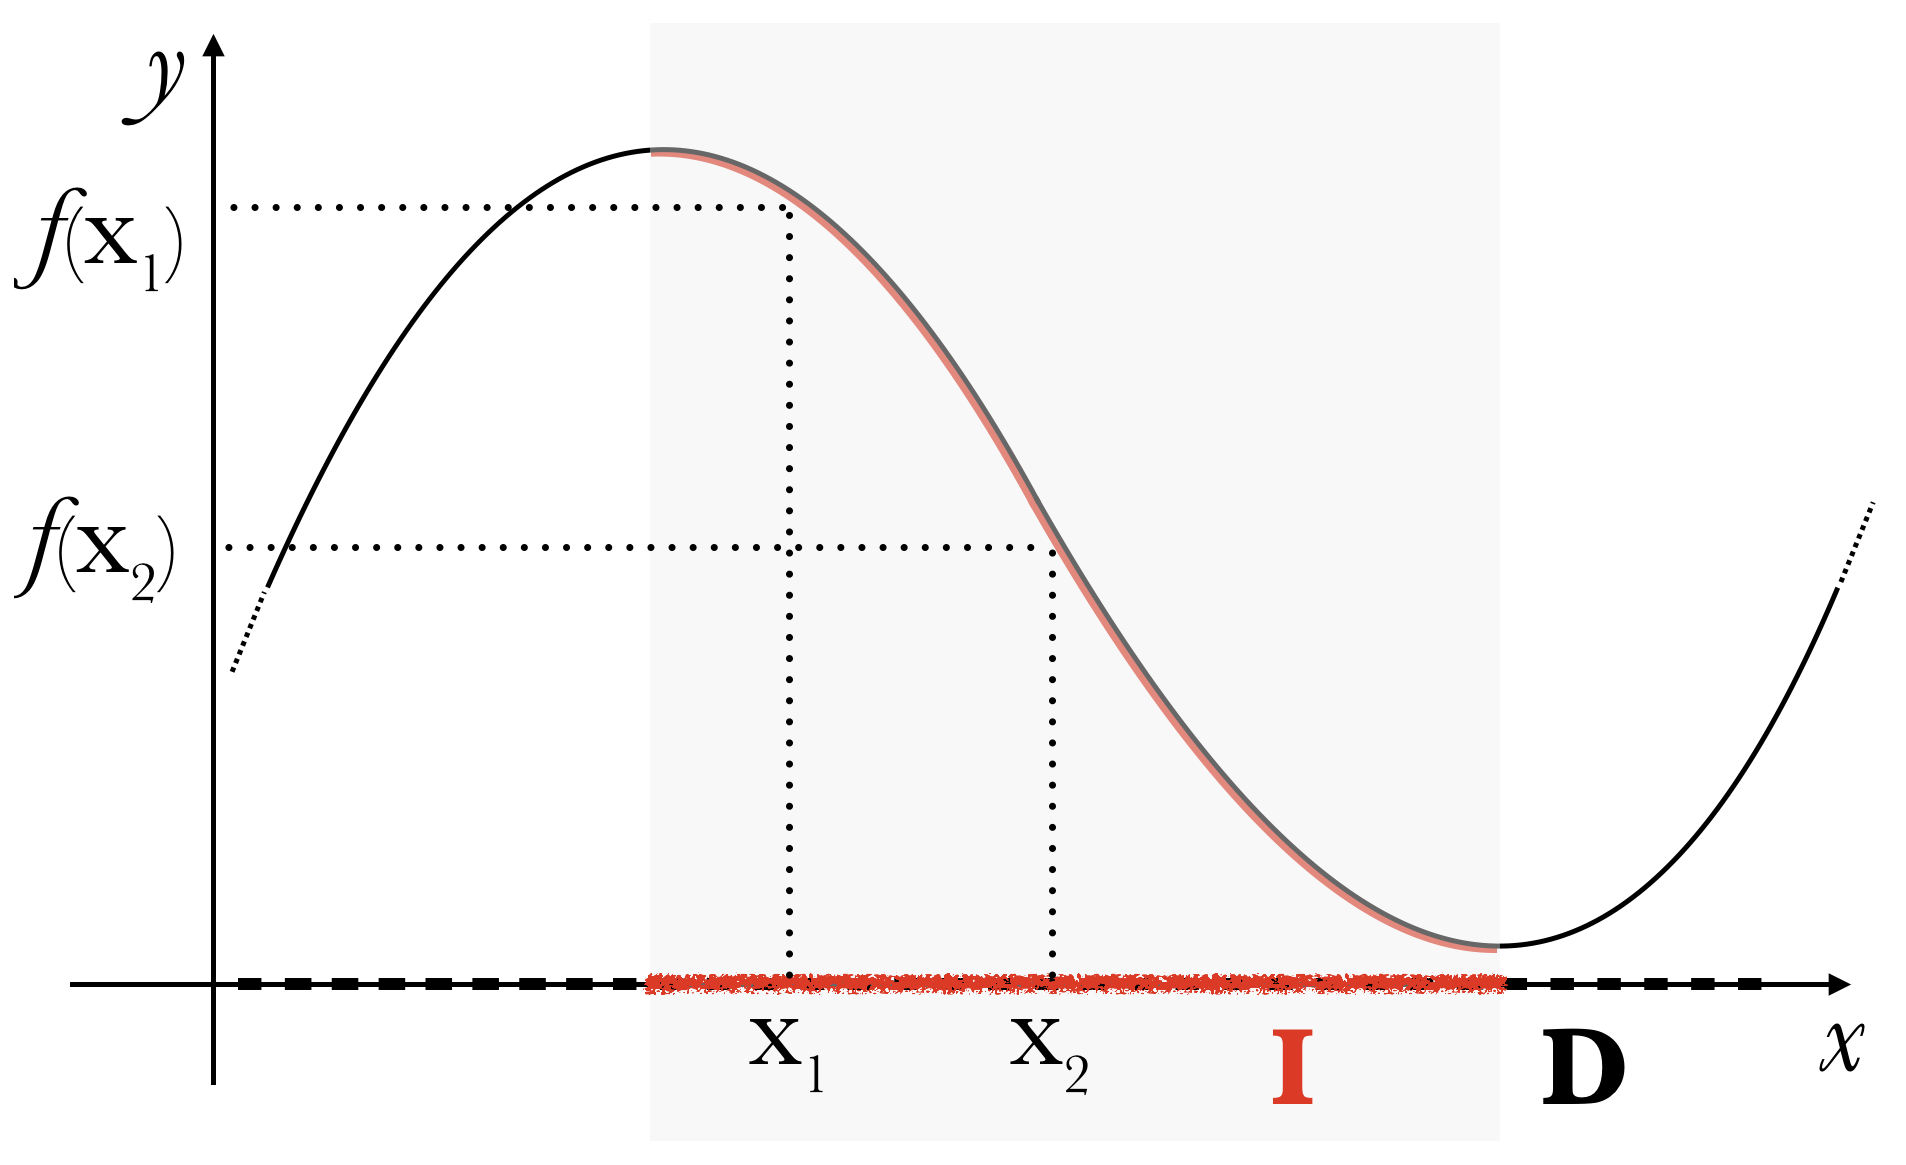
\includegraphics[width=0.55\textwidth]{img/funz_7.png}
  %\caption{}
  %\label{fig:1_2}
\end{figure}
%

\begin{definizione}
Una funzione è non crescente o \textsc{decrescente} in senso lato in un 
intervallo $I$, sottoinsieme di $D$, se\\

$\forall x_1,x_2\in I$  con $x_1<x_2 $ si ha $f(x_1)\geq f(x_2)$\\
\end{definizione}

Una funzione, quindi, si dice monotòna in un intervallo $I$ del suo dominio 
se in $I$ è sempre crescente o decrescente.\\

\begin{esempio}
Individuiamo gli intervalli in cui la funzione rappresentata risulta 
crescente o decrescente.\\
Negli intervalli finiti $x_1<x<x_2$, $x_3<x<x_4$ la funzione risulta essere 
crescente; negli intervalli finiti $x_2<x<x_3$, $x_4<x<x_5$.
% 
\begin{figure}[htpb!]
  \centering
  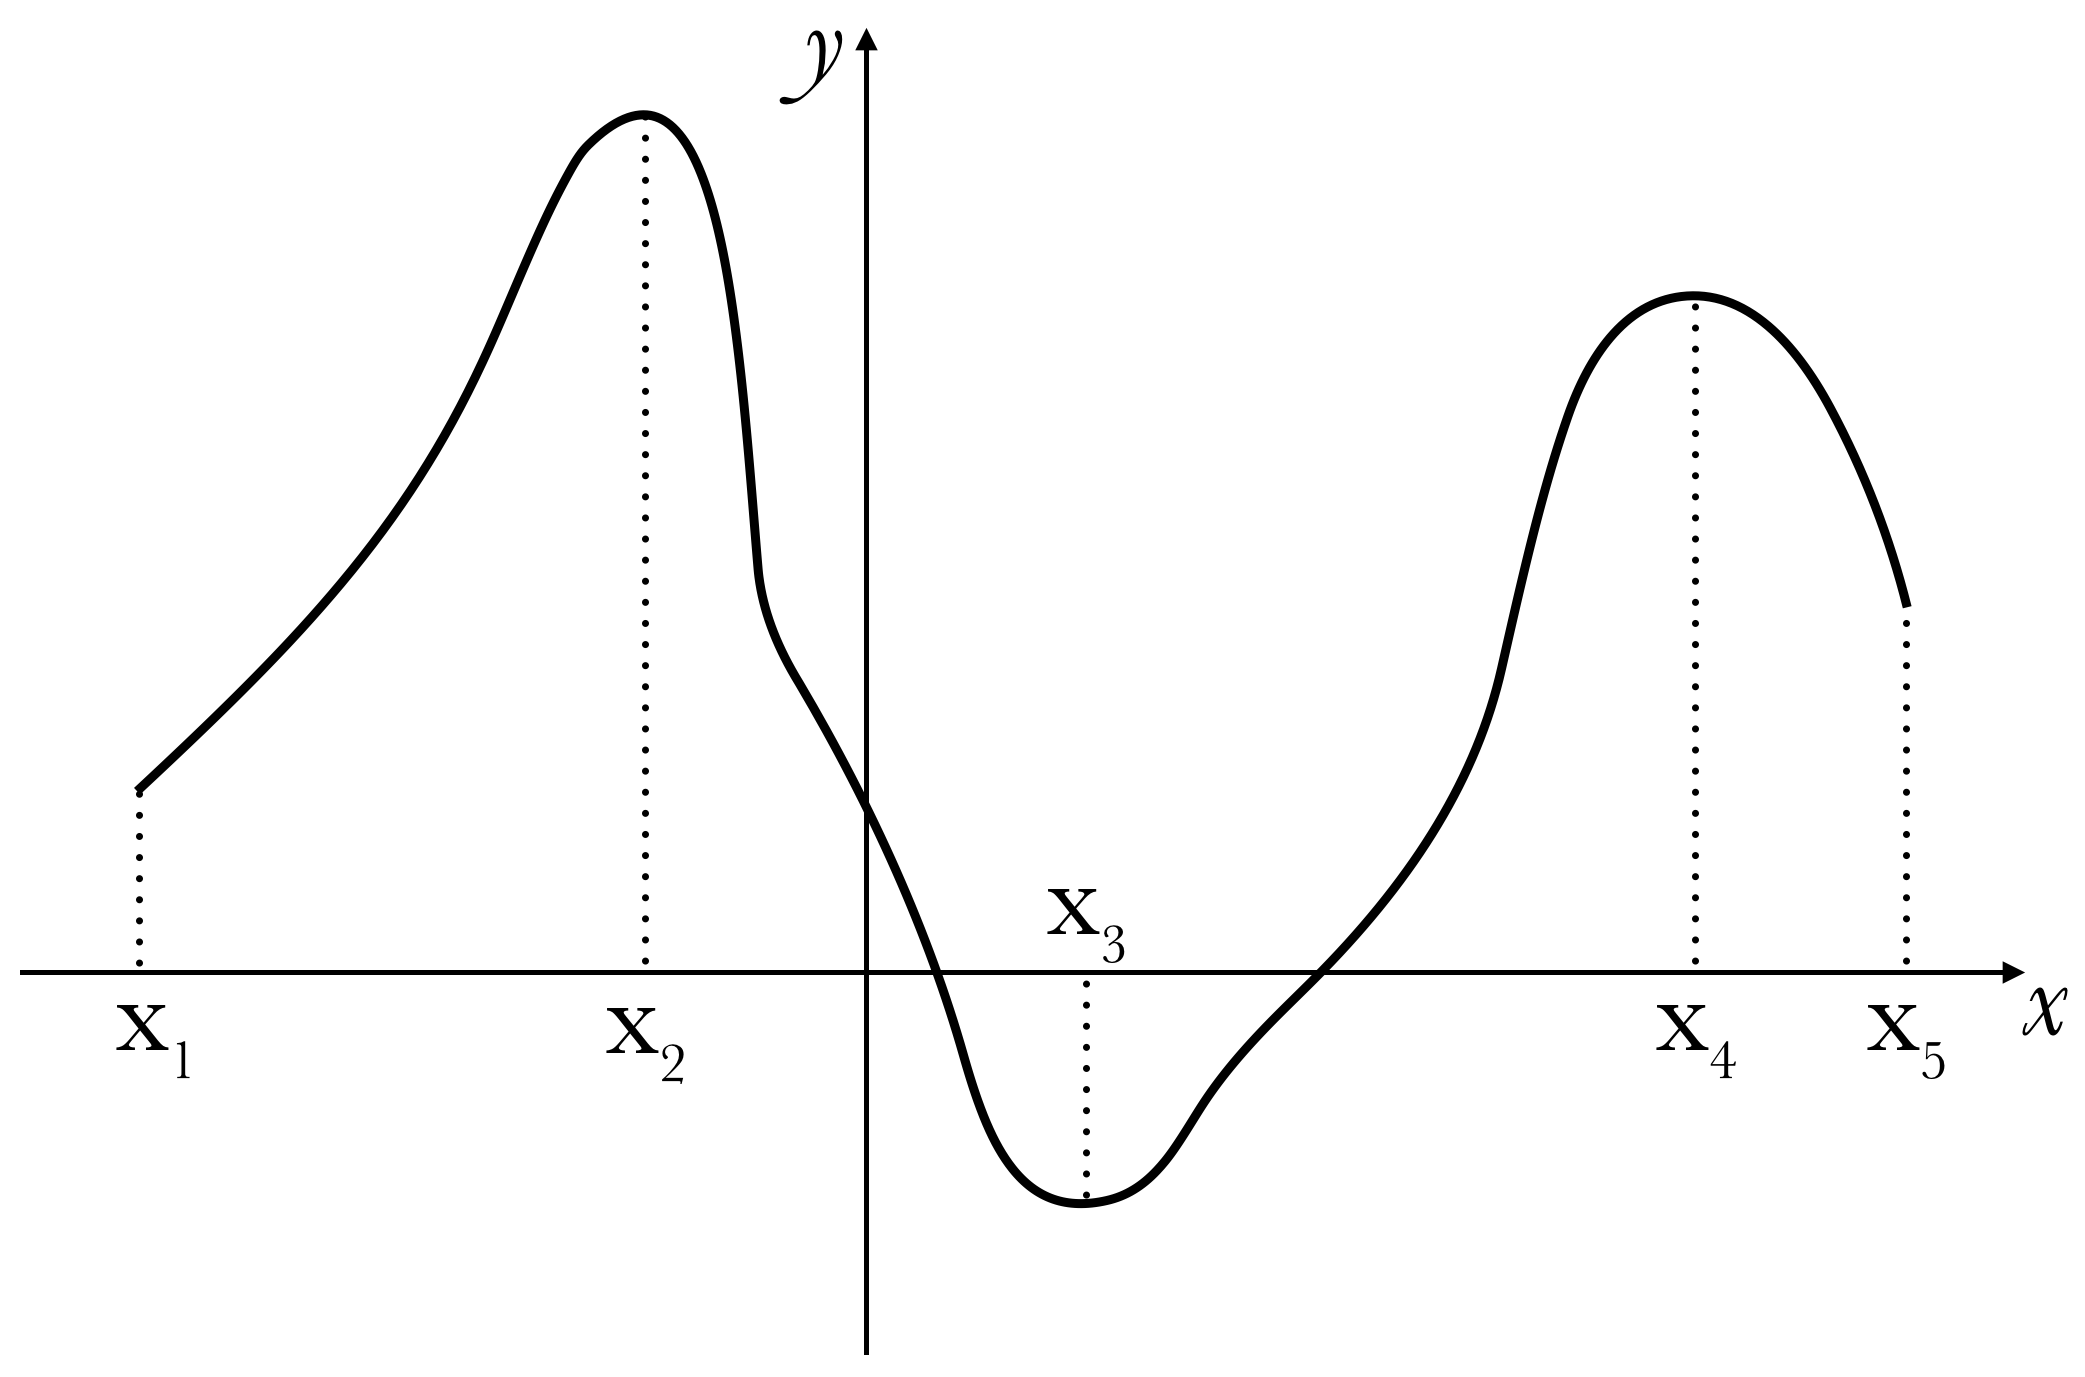
\includegraphics[width=0.4\textwidth]{img/funz_8.png}
  %\caption{}
  %\label{fig:1_2}
\end{figure}
\end{esempio}
\subsection{Parità}
%label{}
La caratteristica della parità va a verificare se il grafico della funzione 
che stiamo studiando è simmetrico rispetto all'asse delle $Y$, cioè il 
grafico è speculare rispetto all'asse, o se il grafico della funzione è 
simmetrico rispetto all'origine. Nel primo caso parleremo di 
\textsc{parità} 
della funzione, nel secondo caso parleremo di \textsc{disparità} della 
funzione.\\

Ovviamente non tutte le funzioni presenteranno questa simmetria, possiamo 
però individuare delle condizioni che, se presenti nella funzione, ci 
assicurano che questa è pari o dispari.\\

\begin{definizione}
Sia data una funzione $y=f(x)$, avente dominio $D$ tale che per ogni $x\in 
D$ 
anche $-x\in D$. Una funzione si dice \textsc{pari} in $D$ se \\
$$f(-x)=f(x)$$
per ogni $x\in D$.
\end{definizione}

\begin{figure}[htpb!]
  \centering
  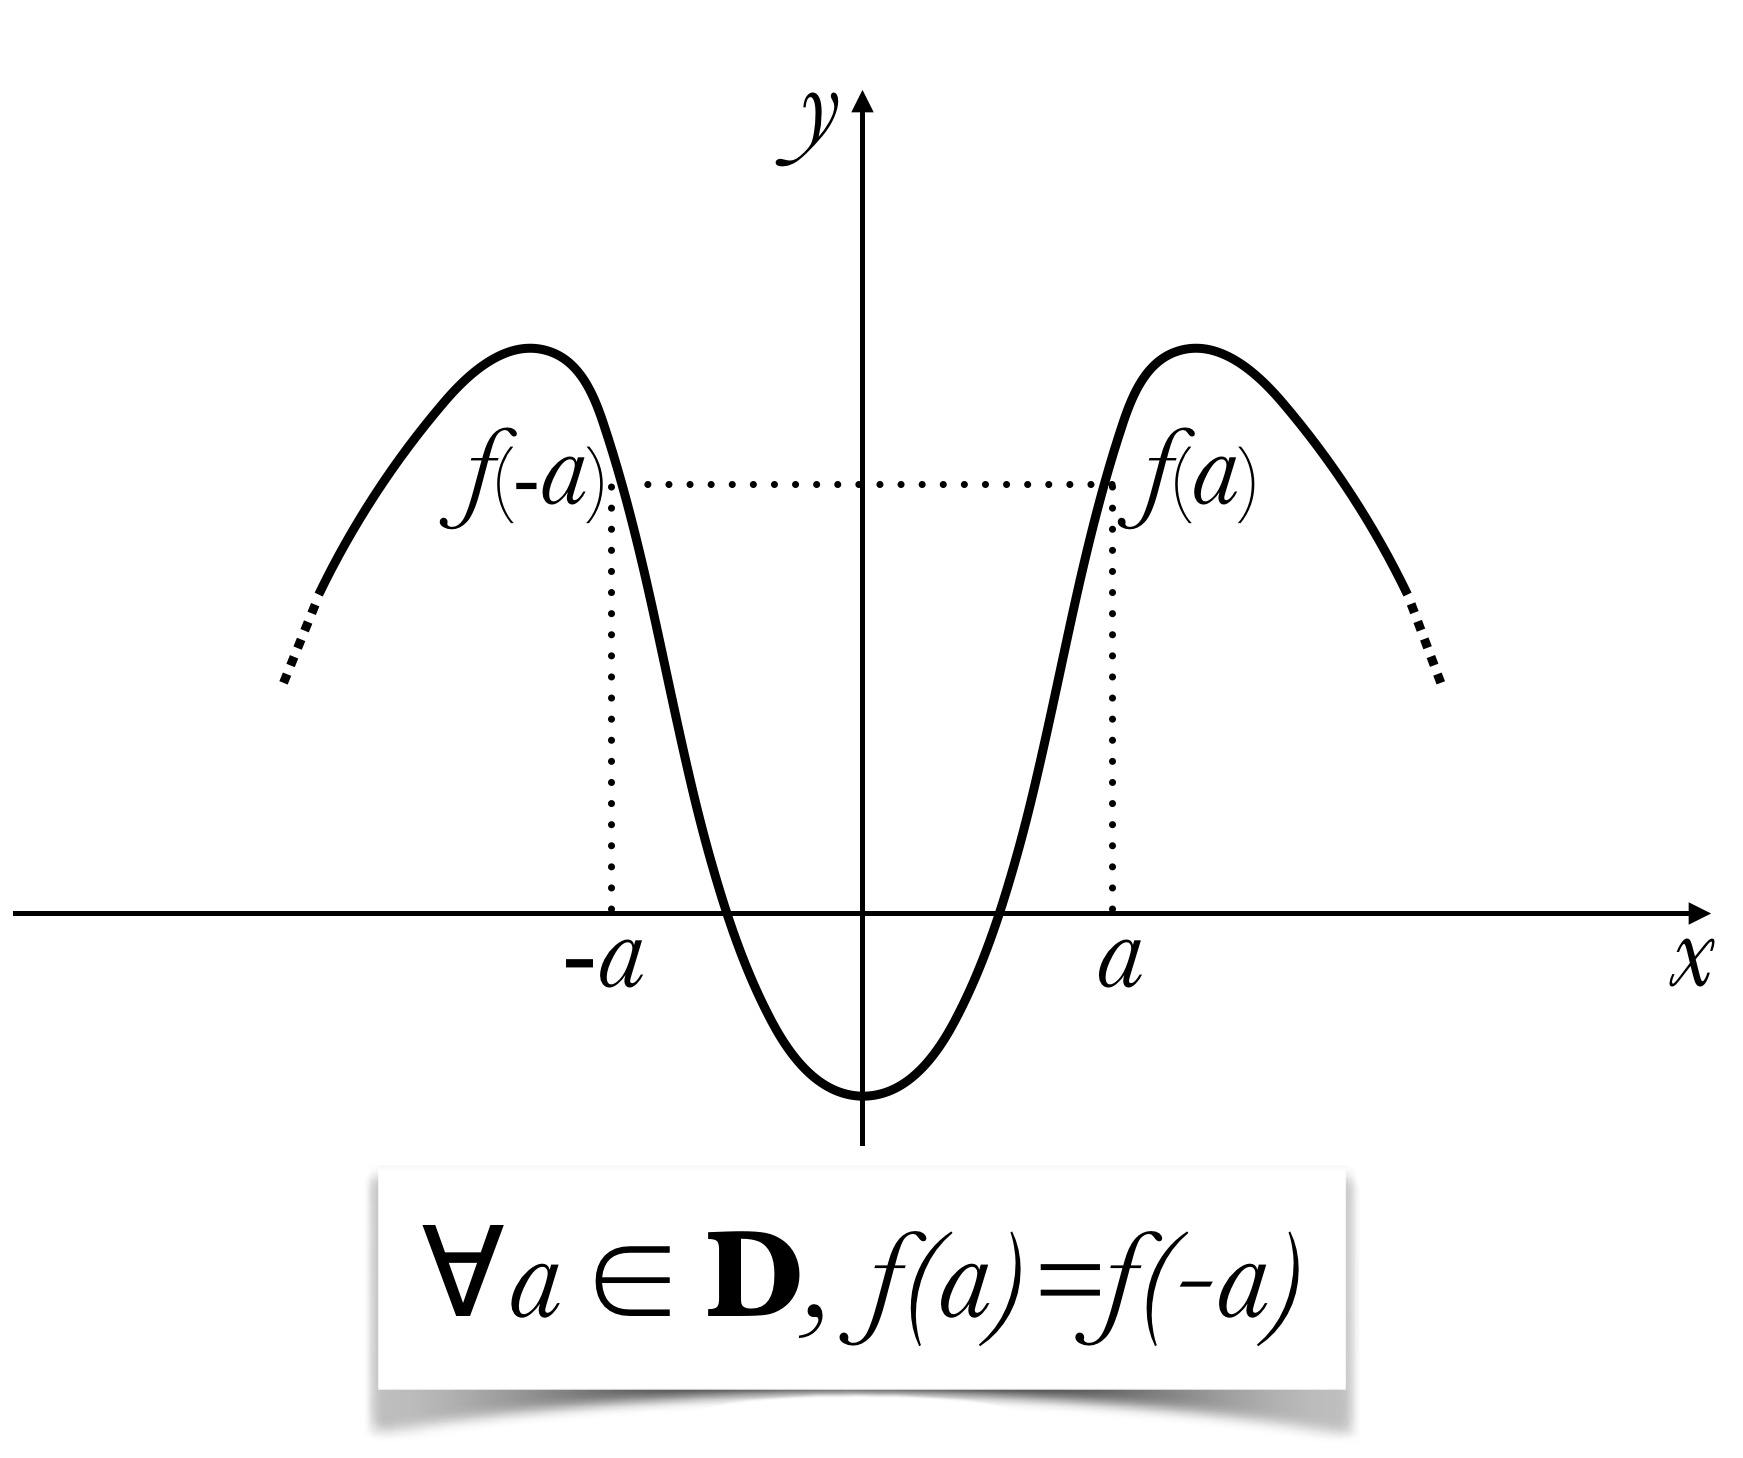
\includegraphics[width=0.5\textwidth]{img/funz_9.png}
  %\caption{}
  %\label{fig:1_2}
\end{figure}
%

Se una funzione è pari, il suo grafico è simmetrico rispetto all'asse $Y$. 
Infatti se $P(x;y)$ appartiene al grafico anche $P'(-x;y)$ vi appartiene. 
Sottolineiamo ancora che la condizione di parità per una funzione è $f(-x)= 
f(x)$.\\   

\begin{esempio} Verificare se una funzione è o non è pari.\\
Per verificare se una funzione è pari basta sostituire nella funzione $-x$ 
al 
posto di $x$ e verificare se la nuova $f(-x)$ è uguale alla funzione di 
partenza, cioè se $f(-x)=f(x)$. Se prendiamo la funzione 
$$f(x)=\frac{x^2+3}{x+2}$$ \underline{non} è pari, infatti 
$$f(-x)=\frac{(-x)^2+3}{(-x)+2}=\frac{x^2+3}{-x+2}\neq f(x).$$
\end{esempio}

\begin{definizione}
Sia data una funzione $y=f(x)$, avente dominio $D$ tale che per ogni $x\in 
D$ 
anche$ -x\in D.$ Una funzione si dice \textsc{dispari} in $D$ se\\
$$f(-x)=-f(x)$$
per ogni $x\in D$.
\end{definizione}

\begin{figure}[htpb!]
  \centering
  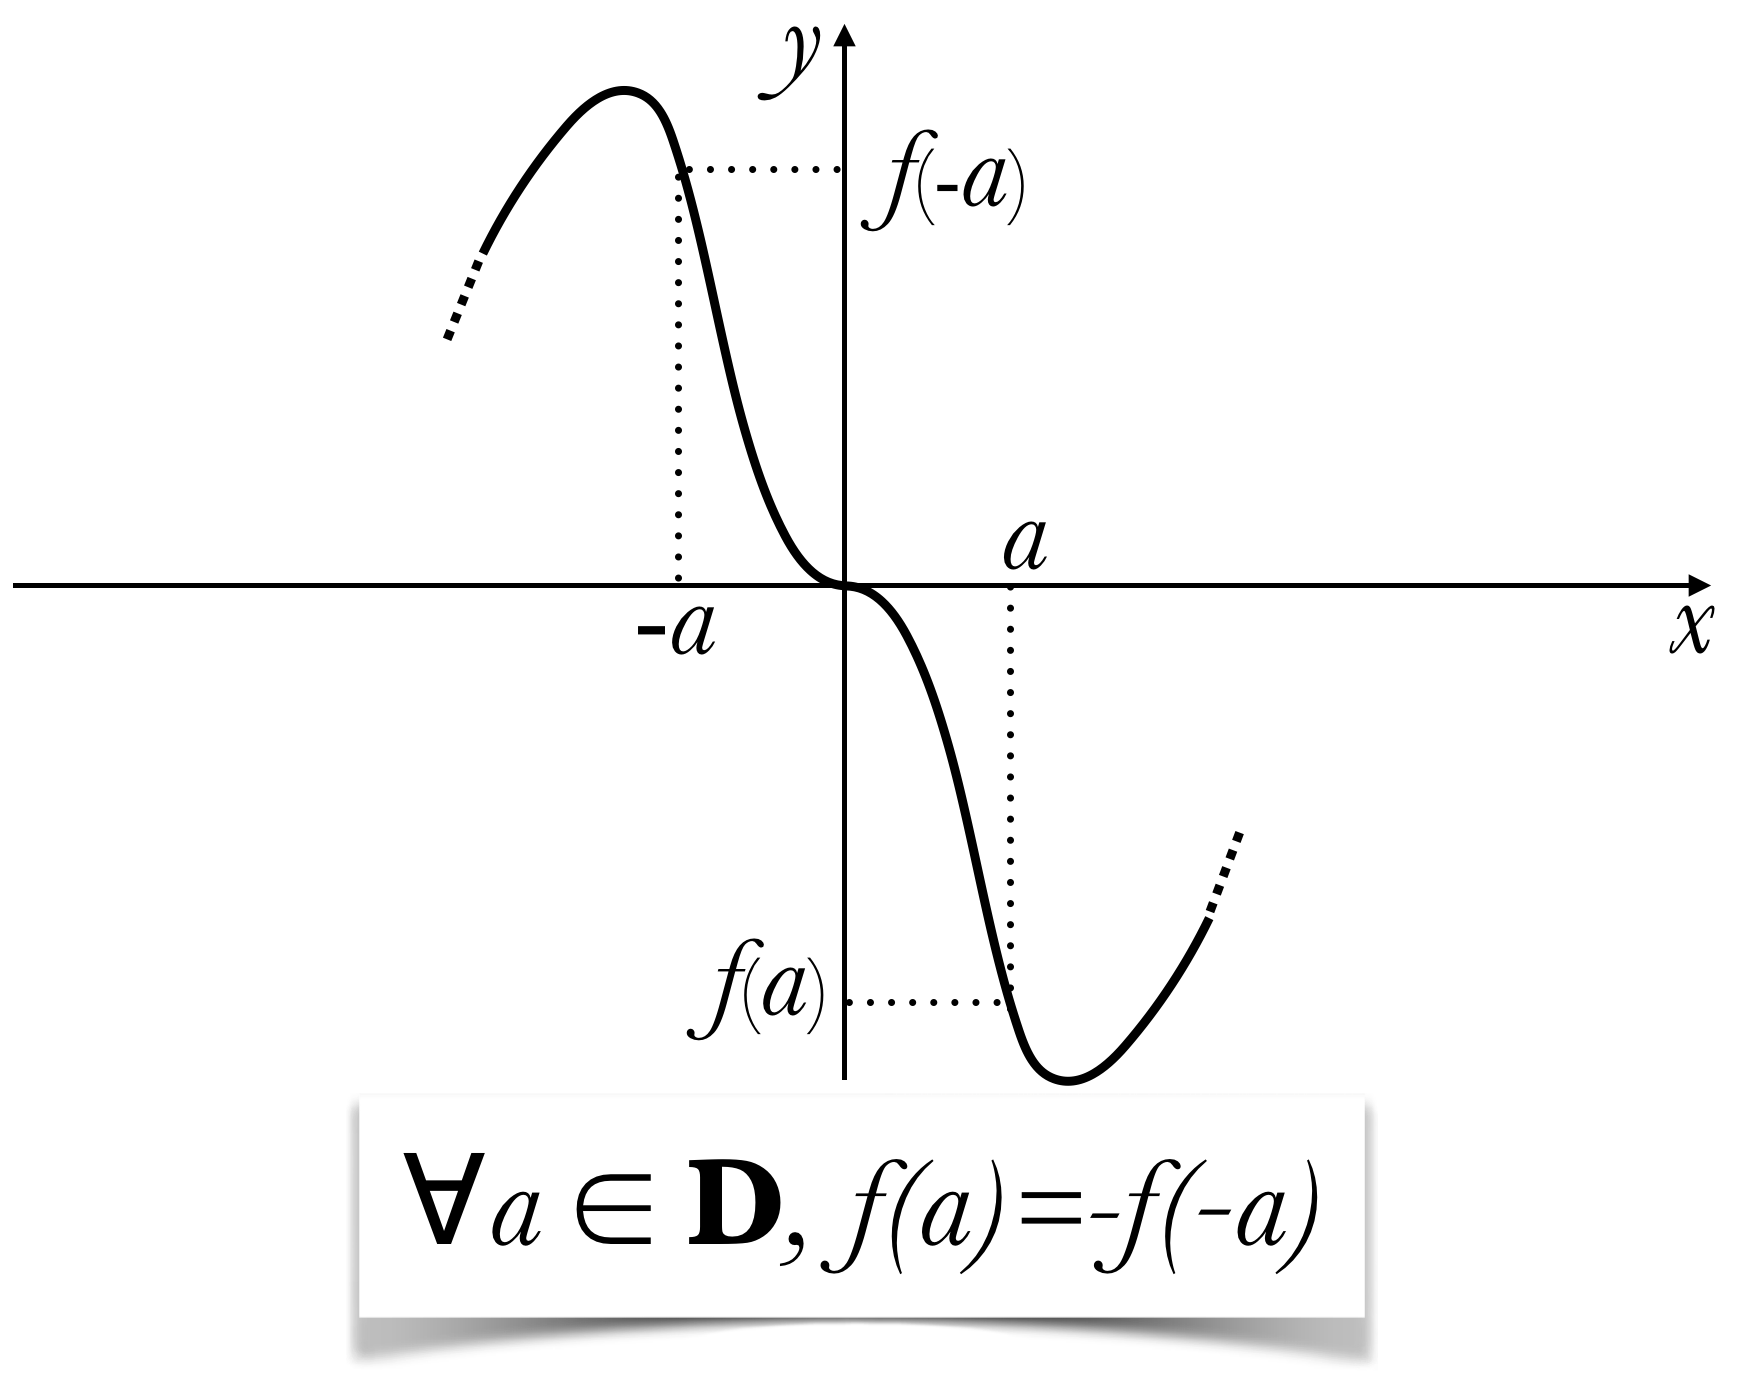
\includegraphics[width=0.5\textwidth]{img/funz_10.png}
  %\caption{}
  %\label{fig:1_2}
\end{figure}
%

Se una funzione è dispari, il suo grafico è simmetrico rispetto 
all'origine. 
Infatti se $P(x;y)$ appartiene al grafico anche $P'(-x;-y)$ vi appartiene. 
Sottolineiamo ancora che la condizione di disparità per una funzione è 
$f(-x)= -f(x)$. \\

\begin{esempio} Verificare se una funzione è o non è dispari.\\
Per verificare se una funzione è dispari basta sostituire nella funzione 
$-x$ 
al posto di $x$ e verificare se la nuova $f(-x)$ è uguale alla funzione di 
partenza cambiata di segno, cioè se $f(-x)=-f(x)$. Se prendiamo la funzione 
$$f(x)=\frac{x}{x^2+2}$$ è dispari, infatti 
$$f(-x)=\frac{(-x)}{(-x)^2+2}=\frac{-x}{x^2+2}=-\frac{x}{x^2+2}= -f(x).$$
\end{esempio}

\subsection{Periodicità}
%label{}
La periodicità di una funzione specifica se questa si ripete uguale a sé 
stessa ad intervalli regolari.\\

\begin{definizione}
Una funzione $y=f(x)$, $f(x): A\to \mathbb{R}$ si dice \textsc{periodica} 
di 
periodo $T>0$ di periodo $T>0$ se$\forall x\in A\rightarrow (x+T)\in A$e 
possiamo scrivere 
 $$f(x+T)=f(x)$$\\
\end{definizione}

\begin{figure}[htpb!]
  \centering
  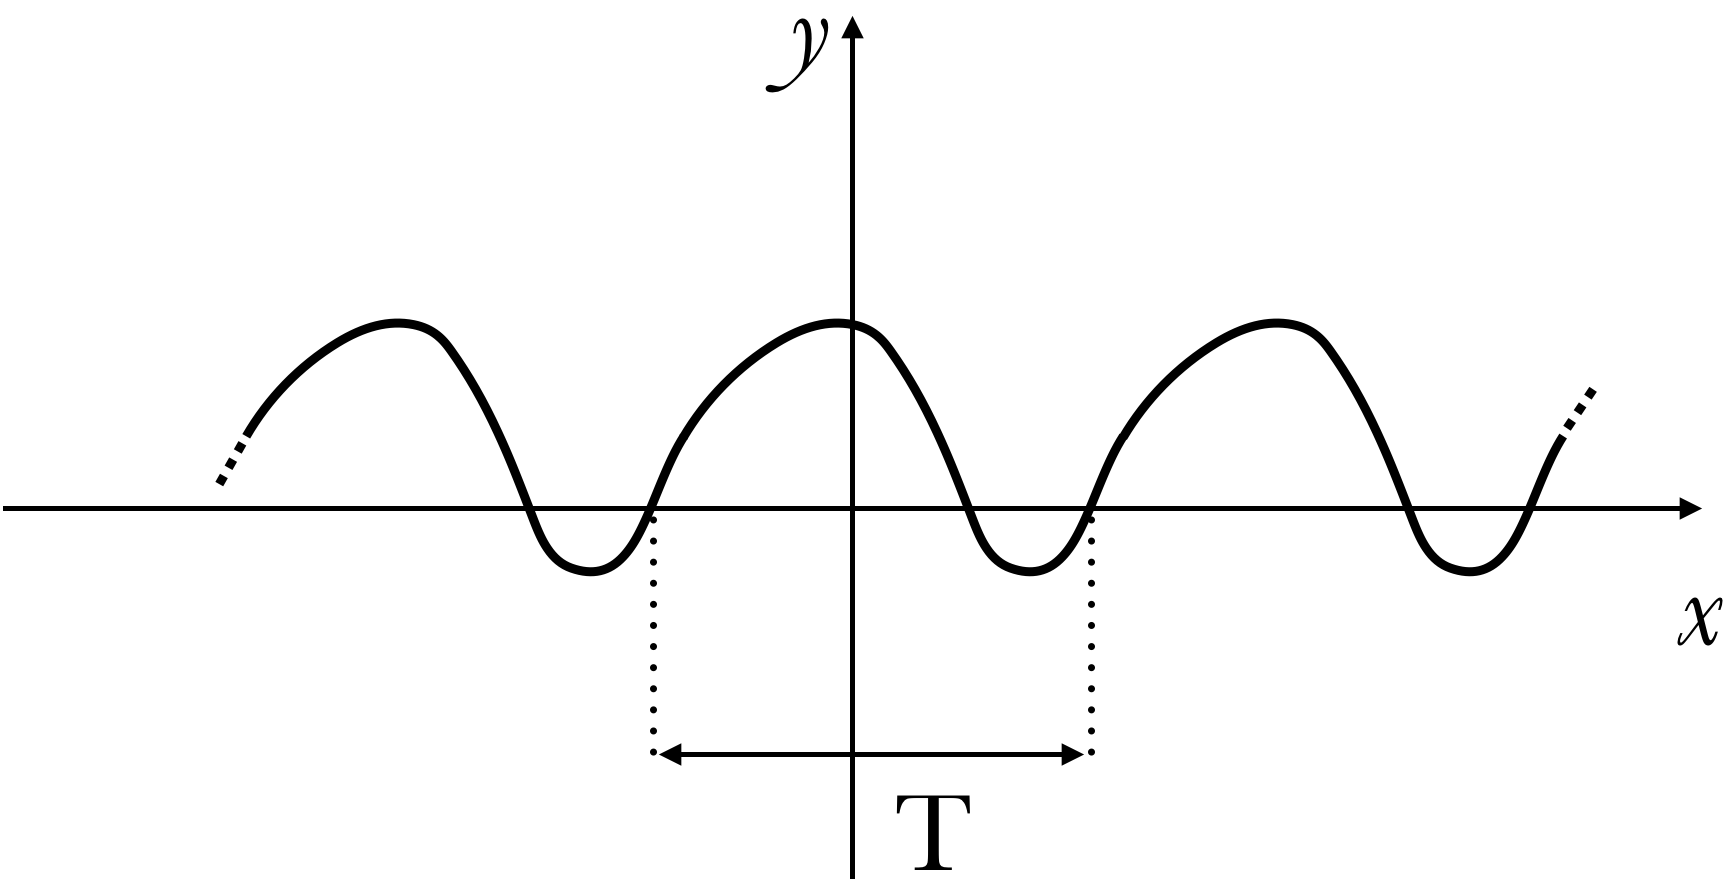
\includegraphics[width=0.45\textwidth]{img/funz_11a.png} \quad 
  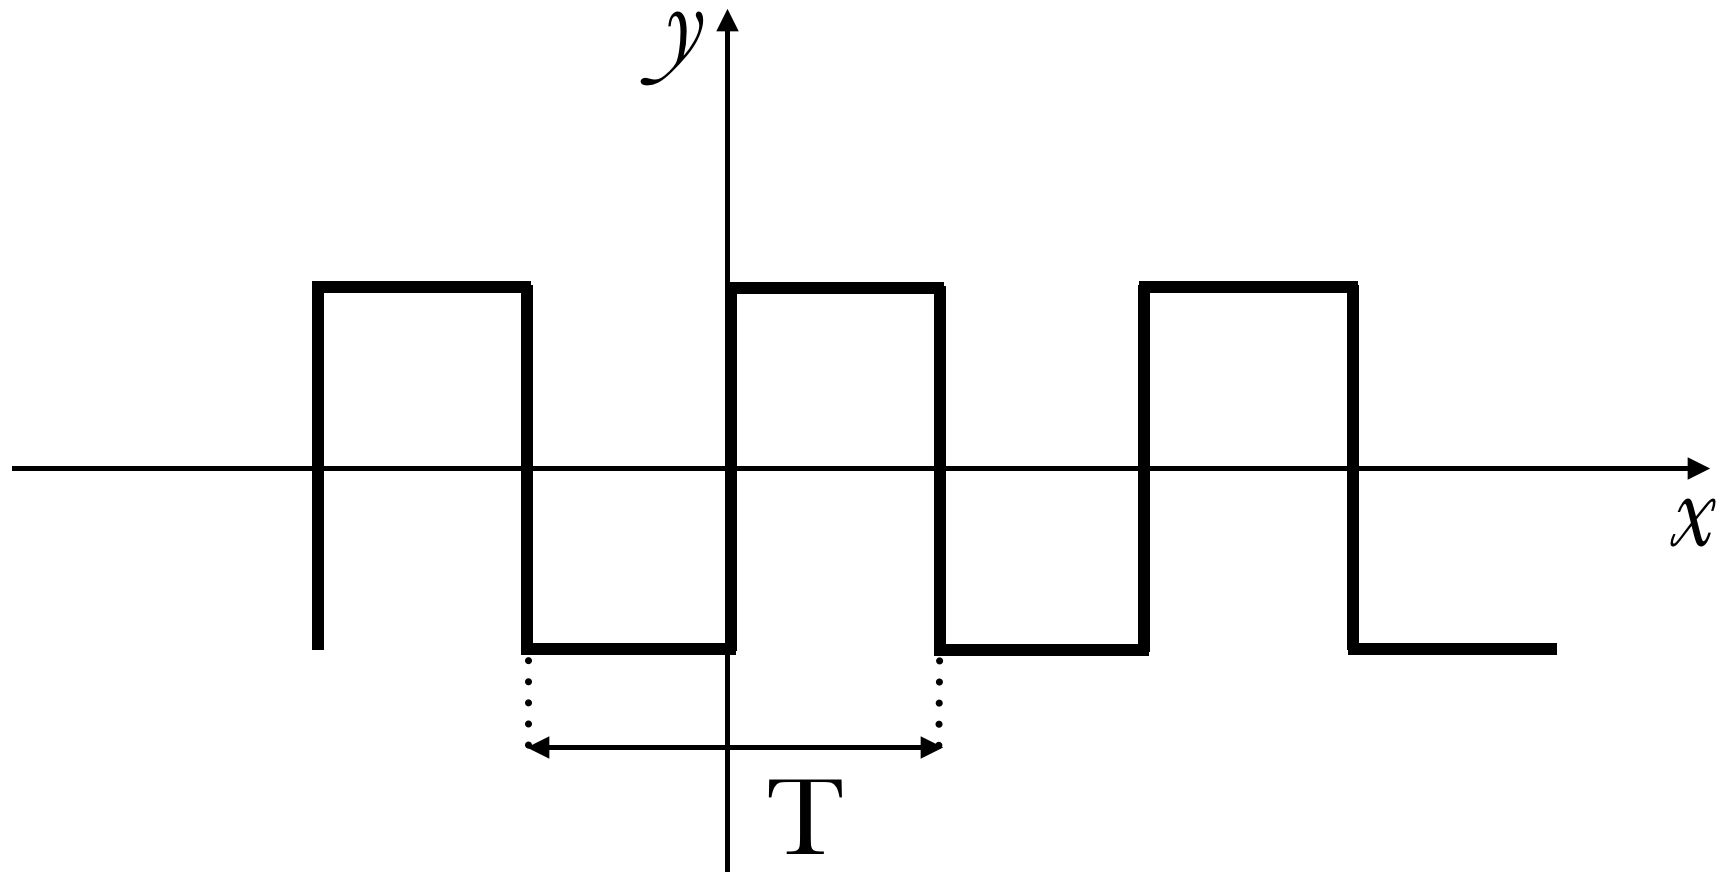
\includegraphics[width=0.45\textwidth]{img/funz_11b.png}
  %\caption{}
  %\label{fig:1_2}
\end{figure}


\begin{esempio} Calcolare il periodo di una funzione.\\
Calcoliamo il periodo della  funzione goniometrica $$y=\sin{7x}$$ con due 
possibili procedure:
\begin{itemize}
  \item[\textsf{Procedura a)}] La funzione ha per definizione periodo 
$T$ se, con $k$ intero,
$$\sin[(7(x+kT)]=\sin4x$$
cioè,
$$\sin[(7x+7kT)]=\sin4x$$
poichè la funzione seno ha periodo $2\pi$, allora
$$\sin[7x+7kT]=\sin[7x+2k\pi]$$
e l'uguaglianza è quindi valida se $7T=2\pi$ da cui
$$T=\frac{2\pi}{7}.$$

  \item[\textsf{Procedura b)}] La funzione $y'=\sin7x'$ viene dalla 
trasformazione della funzione $y=\sin x$, che ha periodo $T=2\pi$, mediante 
una sostituzione $7x'=x$, ovvero $x'=\frac{x}{7}$. Se l'asse delle ascisse 
viene così contratto di un fattore $\frac{x}{7}$, il periodo $T'$ subirà la 
stessa contrazione e pertanto è pari a 
$$T'=\frac{x}{7}(2\pi)=\frac{2\pi}{7}$$
\end{itemize}
\end{esempio}

Se due funzioni $f(x)$ e $g(x)$ hanno periodi diversi $T_f$ e $T_g$, 
rispettivamente, le funzioni $f(x)\pm g(x)$, $f(x)\cdot g(x)$ e 
$\frac{f(x)}{g(x)}$ hanno un periodo pari al m.c.m. tra $T_f$ e $T_g$ 
nell'ipotesi che $\frac{T_f}{T_g}$ sia un numero razionale e diverso da 1. 
Se il rapporto è irrazionale le precedenti combinazioni di funzioni non 
sono periodiche. Se $T_f=T_g$ il periodo globale è minore o uguale del 
periodo comune.\\

\begin{esempio} Calcolare il periodo di combinazioni di funzioni periodiche e 
non periodiche.\\
  \begin{itemize}
  \item[a)] $f(x)=\sin x+\cos 3x$ è periodica di $2\pi$ che è 
il m.c.m. tra $T_f=2\pi$ e $T_g=\frac{2}{3}\pi$.
  
  \item[b)] $f(x)=\sin x+\cos \pi x$ non è periodica perché il 
rapporto $\frac{T_f}{T_g}\notin \mathbb{Q}$, infatti $T_f=2\pi$ e $T_g=2$, 
per cui $\frac{2\pi}{2}=\pi\notin\mathbb{Q}$
  
  \item[c)] $f(x)=\sin \frac{x}{2}-\cos 3x+\tan x$ dove 
$T_{\sin \frac{x}{2}}=4\pi$, $T_{\cos 3x}=\frac{2}{3}\pi$, $T_{\tan}=\pi$
  
  \item[d)] Se consideriamo la funzione 
$$f(x)=\frac{1}{\log[\sin x]}$$ il periodo è $2\pi$
\end{itemize}
\end{esempio}

Se una funzione è periodica i valori delle sue ordinate si ripetono con 
regolarità, quindi per studiarne l'andamento su tutto l'asse reale, basterà 
studiarne l'andamento in un singolo periodo. Ripetiamo ancora che la 
condizione di parità per una funzione è $f(x+T)=f(x)$ con $T$ periodo.
%
%
\subsection{Limitatezza}
%label{}
La limitatezza di una funzione valuta se le ordinate di una funzione 
raggiungono un valore massimo e un valore minimo, oppure non hanno un 
limite.\\


\begin{definizione}
Consideriamo una funzione $f: A\to \mathbb{R}$, la funzione si dice:
  \begin{itemize}
  \item[$\rhd$]\textsc{limitata superiormente} se il suo 
codominio $f(A)$ ha un limite superiore $k$:
$$\exists k\in \mathbb{R} \vert \forall x\in A,\, k\geq f(x)$$ 
  \item[$\rhd$]\textsc{limitata inferiormente} se il suo 
codominio f(A) ha un limite inferiore $k$: 
$$\exists k\in \mathbb{R} \vert \forall x\in A,\, k\leq f(x)$$

  \item[$\rhd$]\textsc{limitata} se il suo codominio $f(A)$ è 
limitato sia superiormente che inferiormente:
$$\exists k\in \mathbb{R},k>0\vert\forall x\in A, \vert f(x)\vert \leq k$$
\end{itemize}

Se una funzione non è limitata da un valore del codominio $k$ si dirà 
illimitata, in particolare:
  \begin{itemize} 
  \item[$\rhd$] \textsc{Illimitata superiormente} se il suo 
codominio $f(A)$ \underline{non} è limitato superiormente;
  \item[$\rhd$] \textsc{Illimitata inferiormente} se il suo 
codominio $f(A)$ \underline{non} è limitato inferiormente;
  \item[$\rhd$] \textsc{Illimitata} se il suo codominio $f(A)$ 
\underline{non} è limitato superiormente \underline{né} inferiormente.
  \end{itemize}
\end{definizione}
%
\begin{esempio} Determinare la limitatezza o illimitatezza di funzioni.\\
In (a) La funzione $f(x)=\log(x)$ è illimitata: né superioremente né 
inferiormente limitata; in (b) La funzione è limitata inferiormente e 
illimitata superiormente; in (c) La funzione $f(x)=\sin{x}$ è limitata sia 
superiormente che inferiormente; in (d) La funzione $f(x)=x^2$ è limitata 
inferiormente e illimitata superiormente.
\begin{figure}[h]
  \centering
  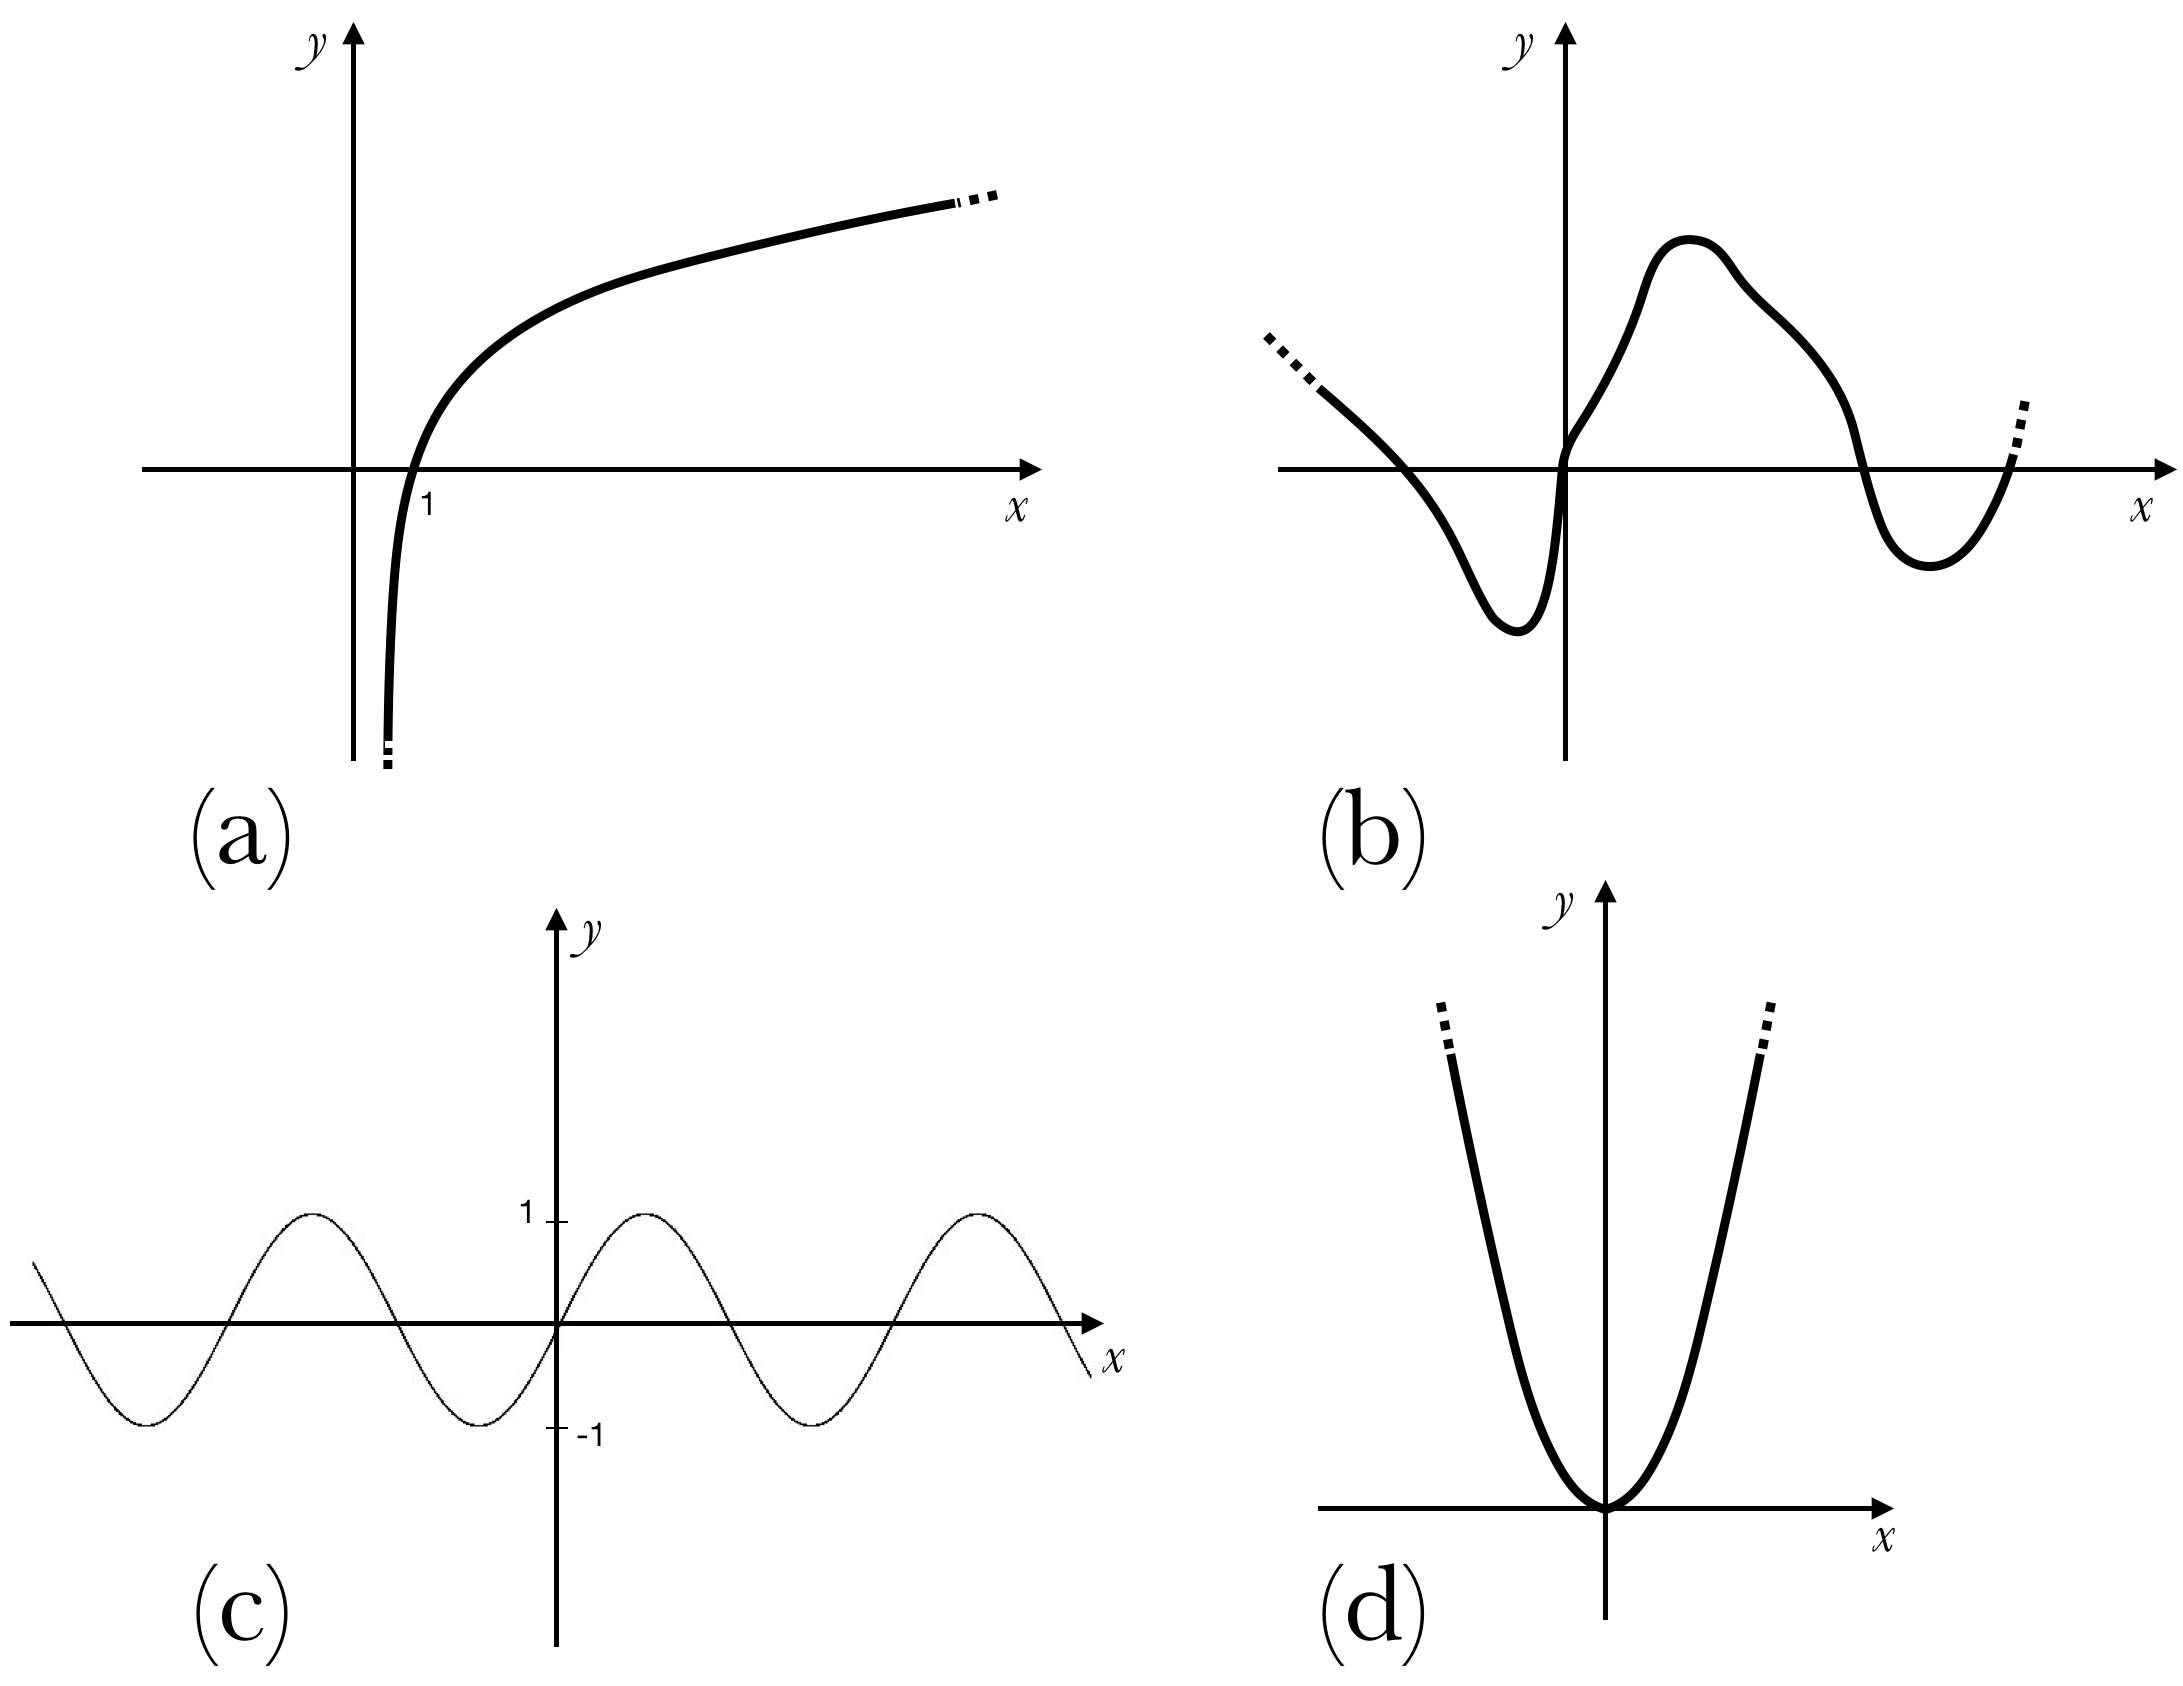
\includegraphics[width=0.85\textwidth]{img/funz_12a.png}
  %\label{fig:1_2}
\end{figure}
\end{esempio}
\newpage
\section{La classificazione delle funzioni}
%label{}
Classifichiamo le possibili funzioni che incontreremo o abbiamo incontrato in 
base alle operazioni che compaiono nella loro espressione analitica. Se 
nell'espressione analitica di una funzione compaiono le operazioni di 
addizione, sottrazione, moltiplicazione, divisione, elevamento a potenza con 
esponente razionale o estrazione di radice siamo di fronte ad una 
\textsc{funzione algebrica}.\\

Le funzioni che non possono essere rappresentate usando solamente le 
operazioni precedentemente ricordate si dicono \textsc{trascendenti}. Tra le 
più note funzioni trascendenti ricordiamo le funzioni goniometriche, quelle 
esponenziali e quelle logaritmiche.\\

A seconda che le funzioni algebriche contengano o meno l'operazione di radice 
e l'operazione di divisione suddividiamo le funzioni algebriche in 
\textsc{razionali fratte}, \textsc{razionali intere} o polinomiali, 
\textsc{irrazionali fratte} e \textsc{irrazionali intere}. \\

\textsf{MEMO!!} Per non creare equivoci ricordiamo che una funzione è 
definita fratta quando il denominatore contiene la variabile indipendente 
$x$, è invece definita irrazionale quando tale variabile appare sotto il 
segno di radice.\\

% TODO non compila!!!!!!!!!!!!!!!!!!!!!!!!!!!!!!!!!!!!!!!!!!!!!!!!!!!
% \Tree [.FUNZIONI [.\textbf{algebriche}  [.razionali fratte intere 
% !{\qbalance} ] [.irrazionali fratte intere !{\qbalance} ] ] 
% [.\textbf{trascendenti} goniometriche esponenziali logaritmiche ] ] \\


\begin{esempio} Classificazione di funzioni.\\
Classifichiamo le seguenti funzioni: 
  \begin{itemize}
  \item[a)] $f(x)=\frac{\sqrt{(x+5)}}{3}$ è una funzione 
irrazionale intera, infatti pur avendo un denominatore, questo non contiene 
la variabile indipendente $x$;
  
  \item[b)] $g(x)=e^{\frac{x}{x-1}}$ è una funzione 
trascendente di tipo esponenziale;

  \item[c)] $h(x)=\sqrt{2}x+4x$ è una funzione razionale 
intera, in quanto la radice compare solo nel numero irrazionale  a 
coefficiente della $\sqrt{2}$ $x$.
  \end{itemize}
\end{esempio}

\section{Funzioni inverse, composte e uguali}
%label{}
Nella rappresentazione insiemistica studiata finora abbiamo sempre visto le 
frecce partire dall'insieme $A$ per arrivare nell'insieme $B$. Esiste una 
possibile lettura al contrario? Se le frecce partissero da $B$, dalle $y$ per 
arrivare alle $x$, ci troveremmo ancora in presenza di una funzione?

\begin{definizione}
Sia $f : A\to B$ una funzione biiettiva. Si dice funzione inversa di $f$ la 
funzione $f^{-1} : B\to A$ che associa a ogni $y$ di $B$ il valore $x$ di $A$ 
tale che $y=f(x)$.
\end{definizione}

\begin{figure}[htpb!]
  \centering
  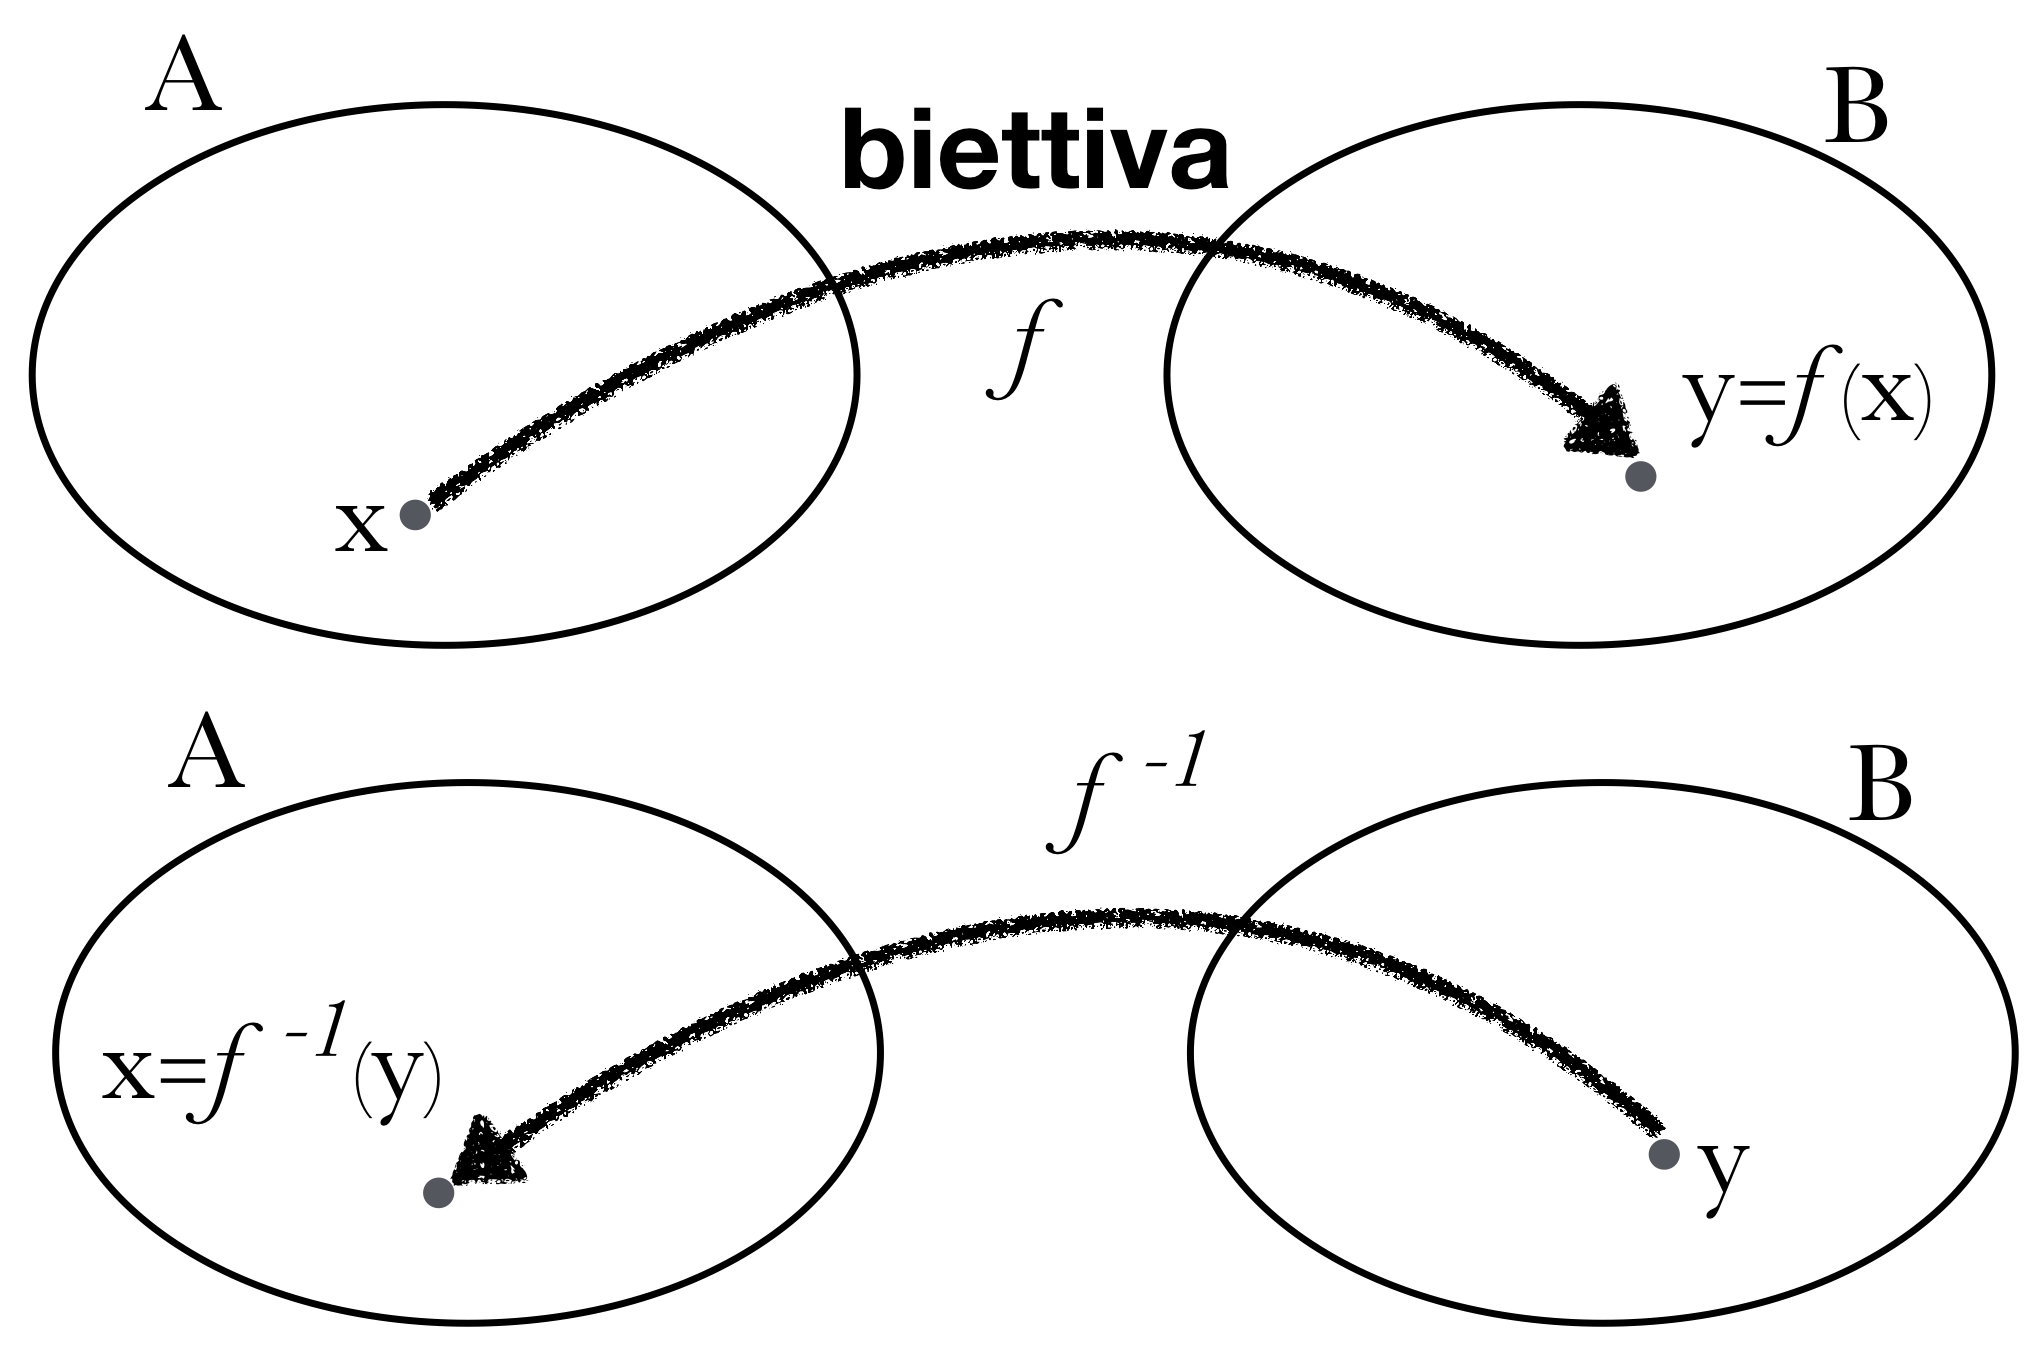
\includegraphics[width=0.45\textwidth]{img/funz_12.png} 
  %\caption{}
  %\label{fig:1_2}
\end{figure}

Notiamo che se una funzione ammette inversa si dice \textsc{invertibile}. 
Significativa è, poi, la relazione tra i codomini e i domini delle due 
funzioni, $f$ e la sua inversa: il dominio di $f^{-1}$ è l'immagine di $f$ e 
l'immagine di $f^{-1}$ è il dominio di $f$.\\

\begin{esempio} Calcolare  e graficare l'inversa di una funzione, verificando 
che sia invertibile.\\ 
Consideriamo la funzione biiettiva $f:\mathbb{R}\to\mathbb{R}$ definita da
$$f(x)=y=3x+2$$
Possiamo ottenere la sua inversa $f^{-1}$ nel seguente modo:
  \begin{itemize}
  \item ricaviamo $x$ in funzione di $y$ dalla relazione 
precedente
$$x=\frac{y-2}{3}$$
  \item sostituiamo la $x$ con $y$ e viceversa.
  \begin{figure}[htpb!]
  \centering
  
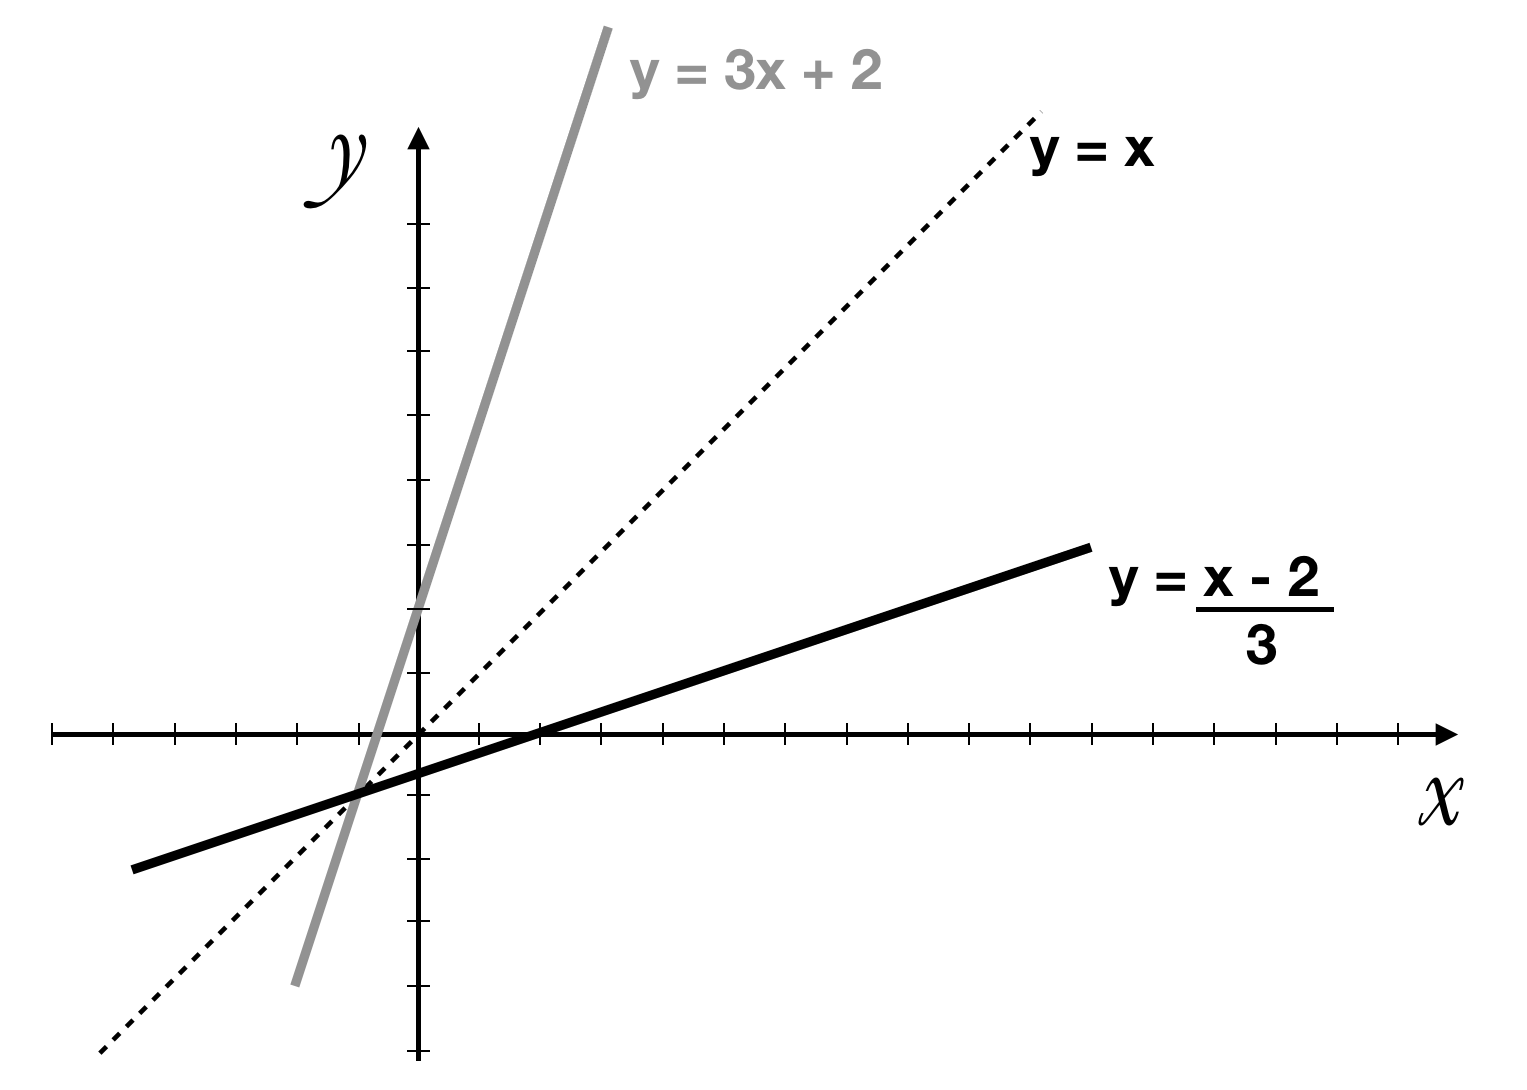
\includegraphics[width=0.5\textwidth]{img/funz_13.png} 
  %\caption{}
  %\label{fig:1_2}
  \end{figure}
  \item notiamo che il grafico della funzione inversa
$$f^{-1}(x)=\frac{x-2}{3}$$
è simmetrico a quello di $f(x)$ rispetto alla bisettrice del primo e terzo 
quadrante, la retta di equazione $y=x$
  \end{itemize}
\end{esempio}

\begin{esempio} Disegnare l'inversa di una funzione che originariamente non 
sia invertibile nel suo dominio. 

La funzione $f:\mathbb{R}\to\mathbb{R}$ tale che $$f(x)=x^2+1$$.
\begin{itemize}
  \item $f$ non ammette funzione inversa perché non è biiettiva, in 
quanto non è iniettiva.
  \begin{figure}[htpb!]
  \centering
  
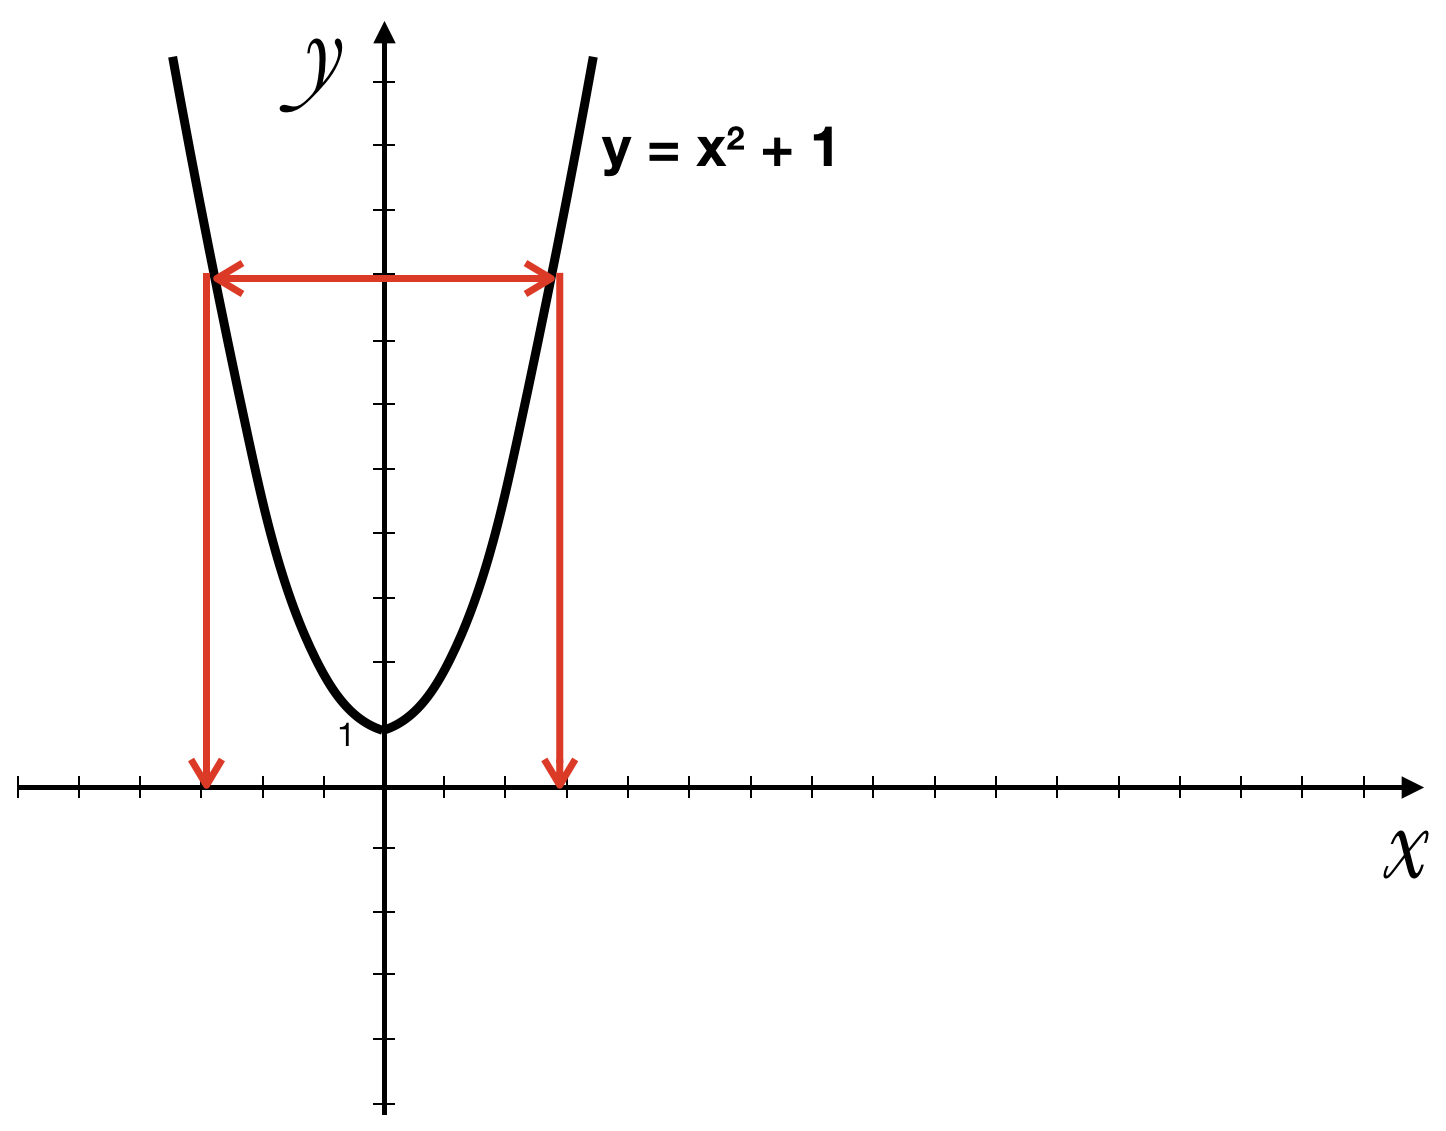
\includegraphics[width=0.45\textwidth]{img/funz_14a.png} %\quad
  
%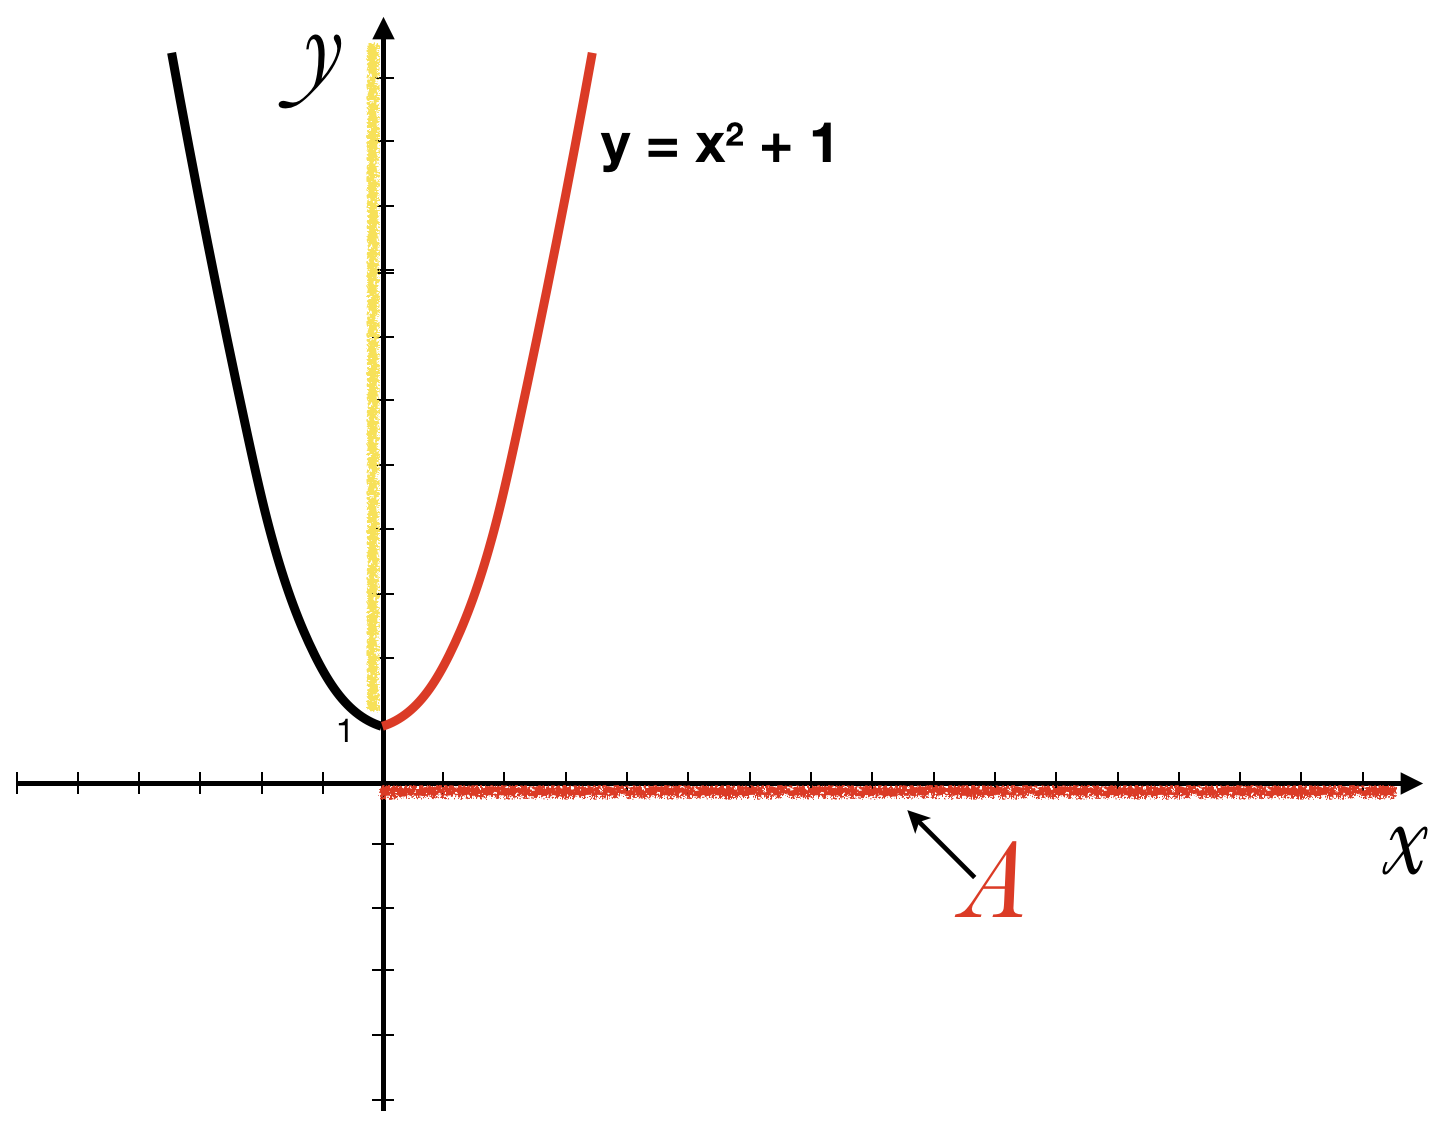
\includegraphics[width=0.7\textwidth]{img/funz_14b.png} \quad
  
%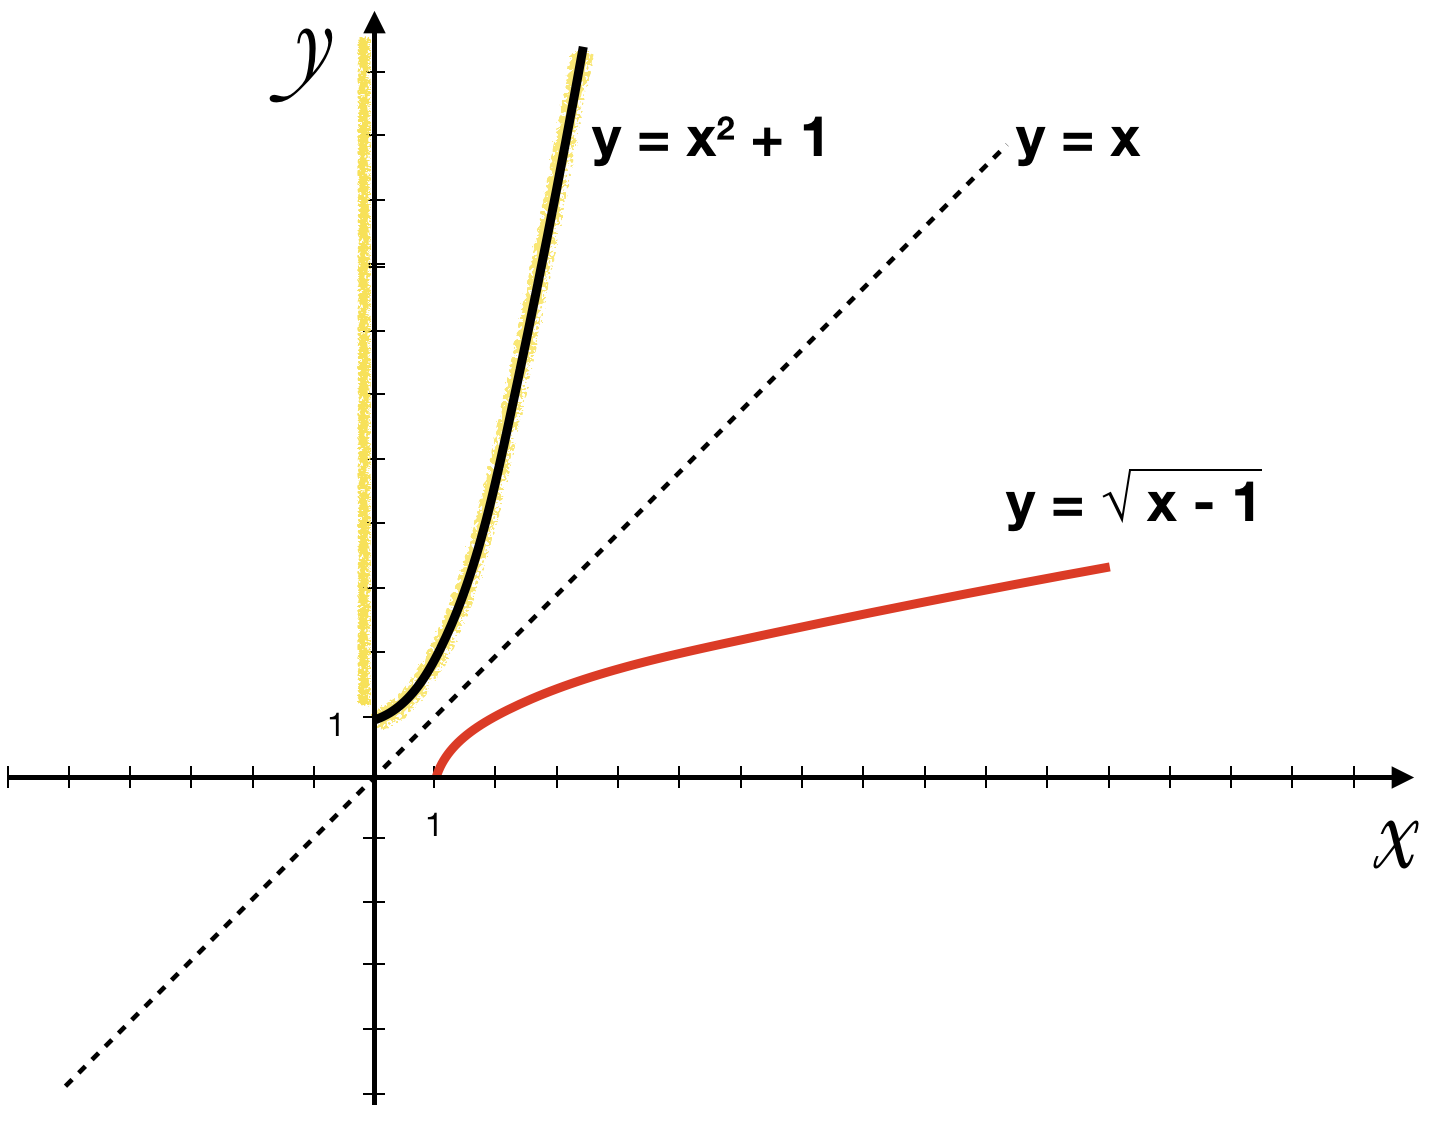
\includegraphics[width=0.7\textwidth]{img/funz_14c.png} 
  %\caption{}
  %\label{fig:funz_14abc}
  \end{figure}
  \item Se $f$ non è biiettiva e quindi non è invertibile, possiamo 
operare una \textsc{restrizione del dominio} a un sottoinsieme in cui $f$ 
risulti biiettiva.
  \begin{figure}[htpb!]
  \centering
  
%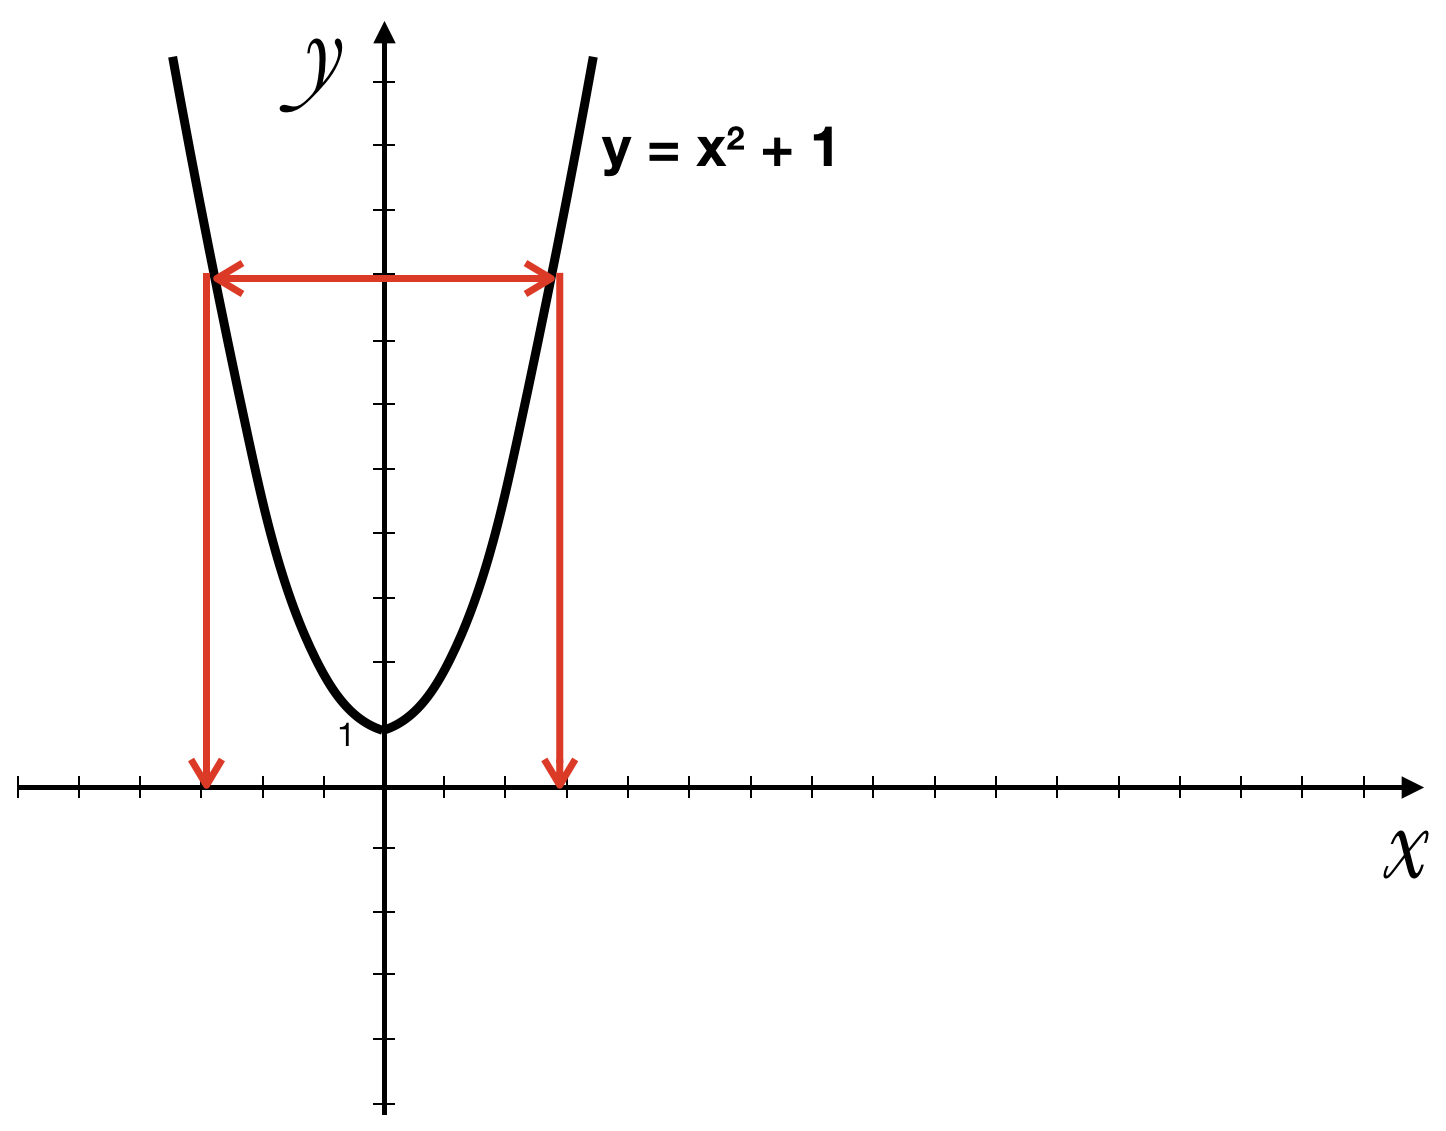
\includegraphics[width=0.7\textwidth]{img/funz_14a.png} %\quad
  
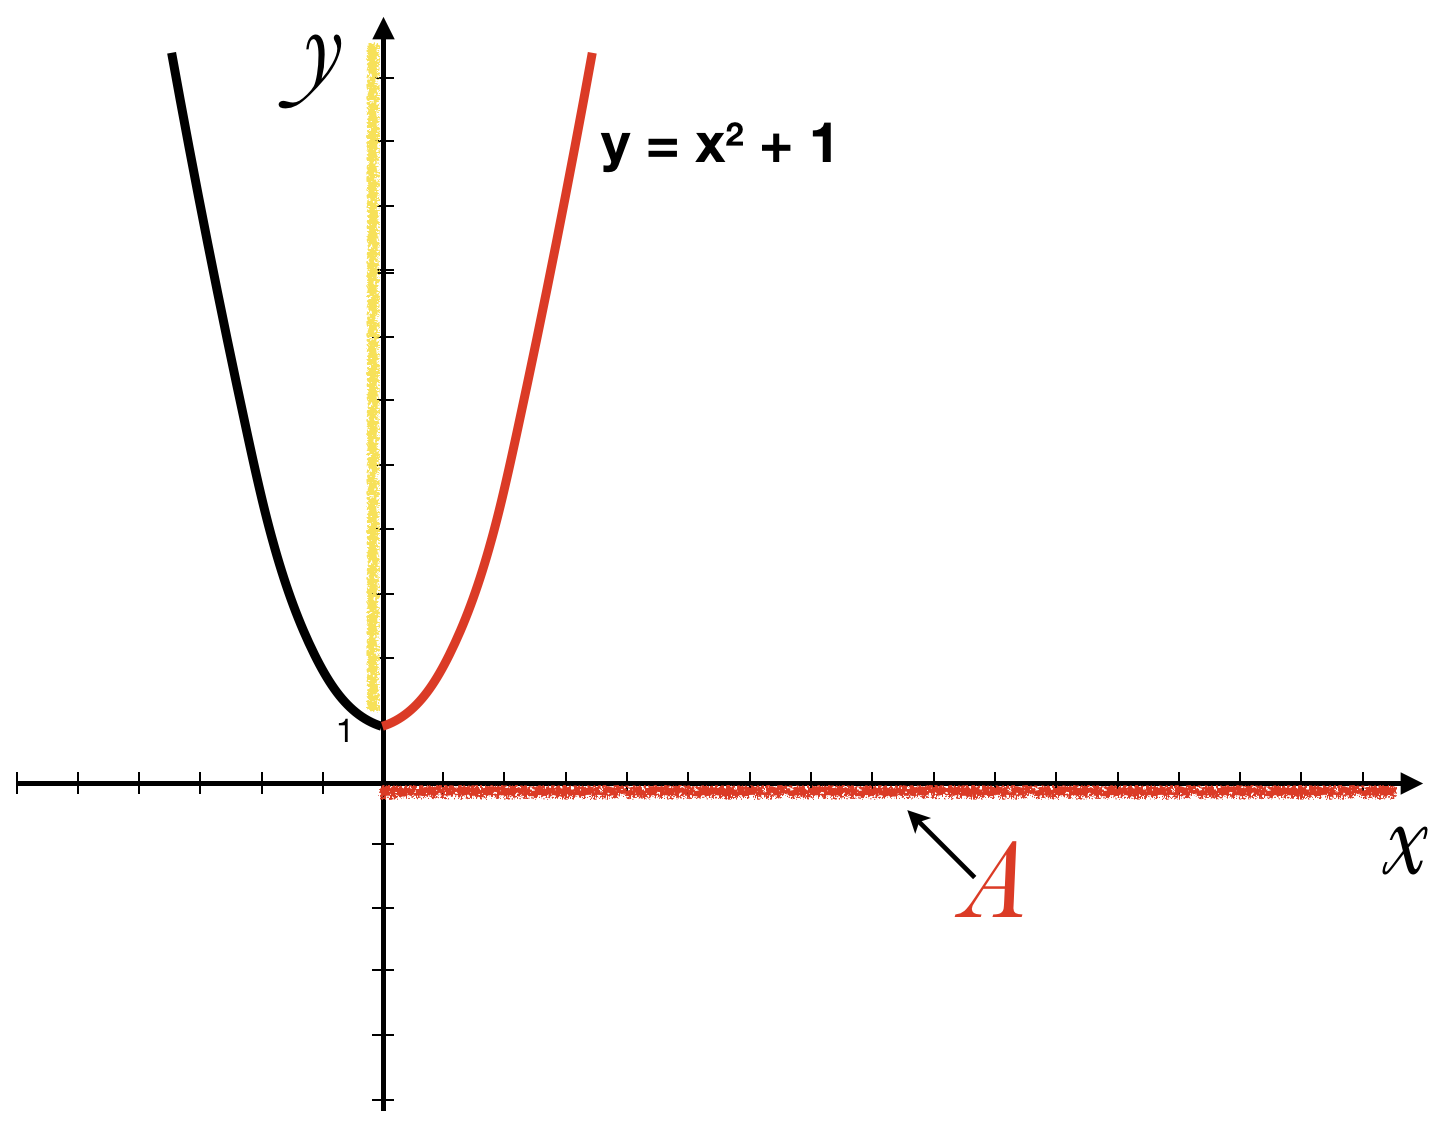
\includegraphics[width=0.45\textwidth]{img/funz_14b.png} %\quad
  
%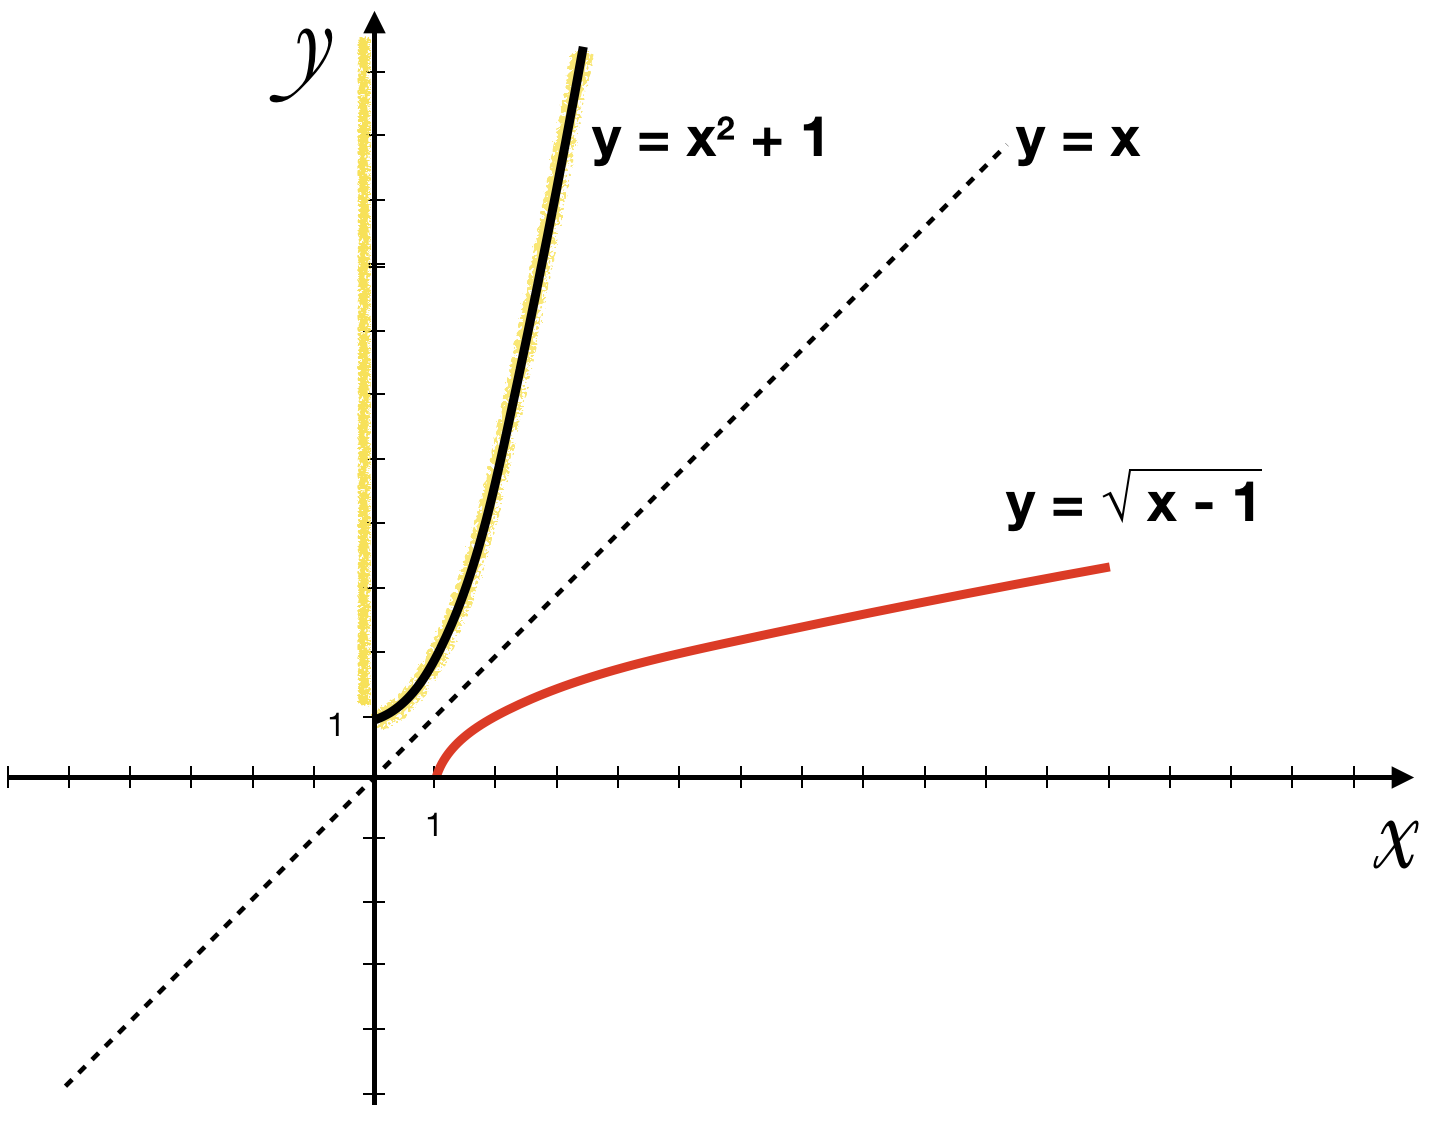
\includegraphics[width=0.7\textwidth]{img/funz_14c.png} 
  %\caption{}
  %\label{fig:funz_14abc}
  \end{figure}
  \item Scelgo solo una parte del dominio che chiamo $A$ e disegno 
l'inversa riflettendo la porzione di funzione biiettiva rispetto alla 
bisettrice del primo e terzo quadrante, la retta di equazione $y=x$.
  \begin{figure}[htpb!]
  \centering
  
%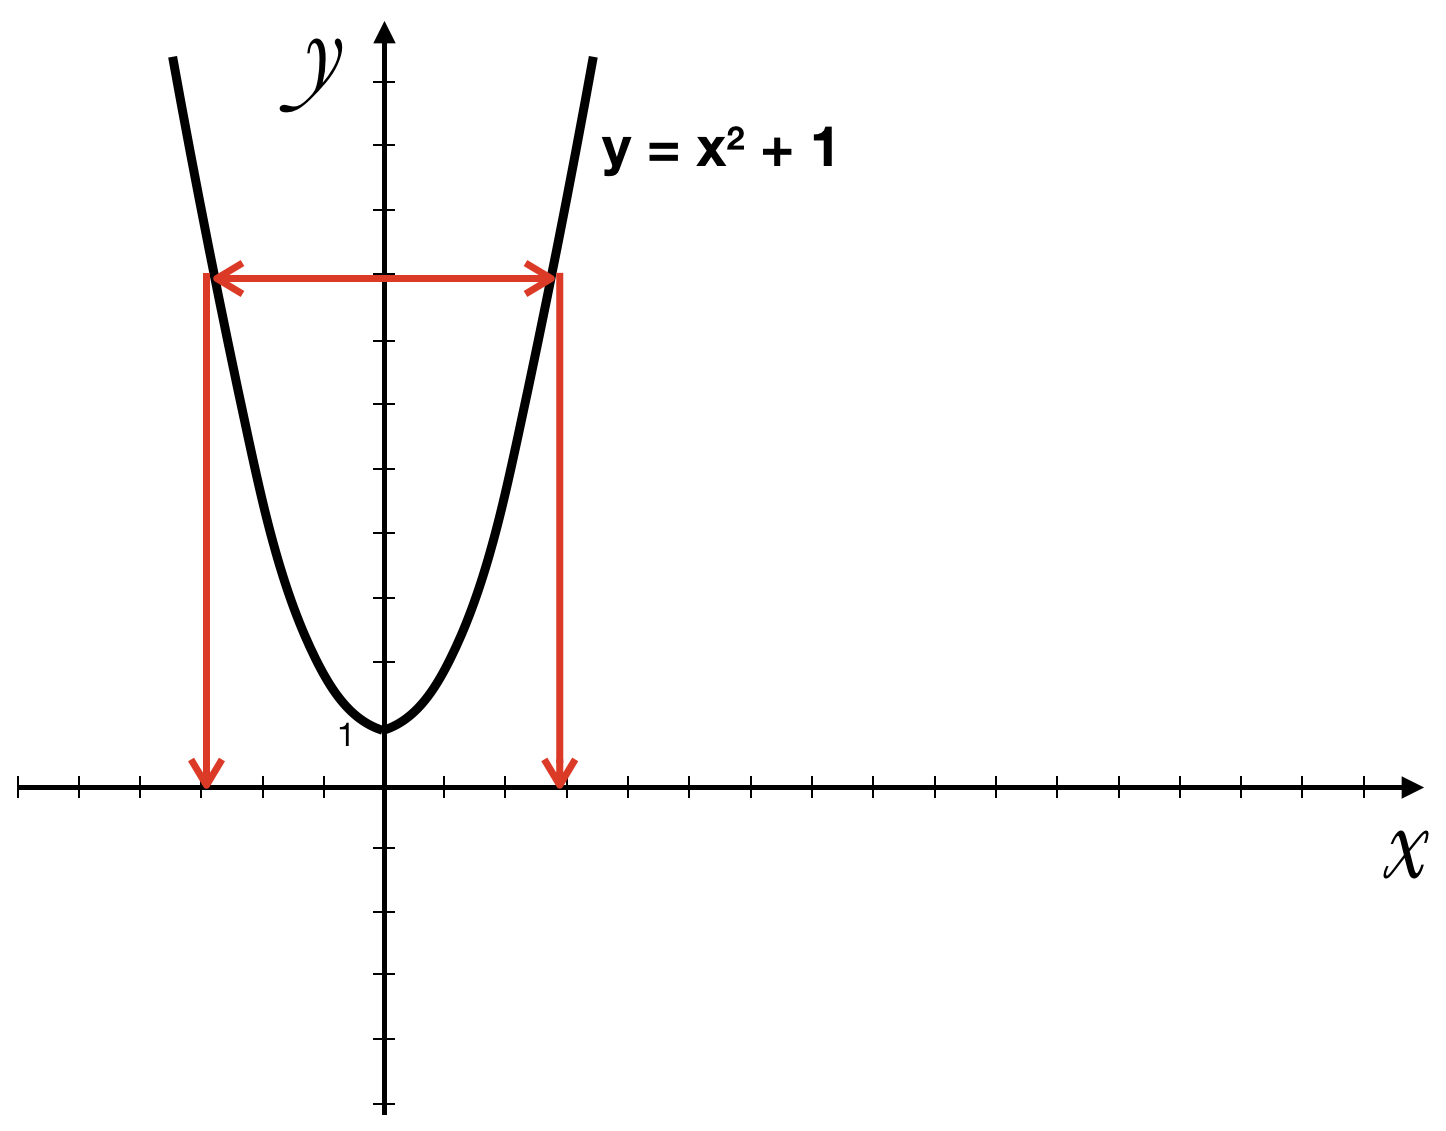
\includegraphics[width=0.7\textwidth]{img/funz_14a.png} \quad
  
%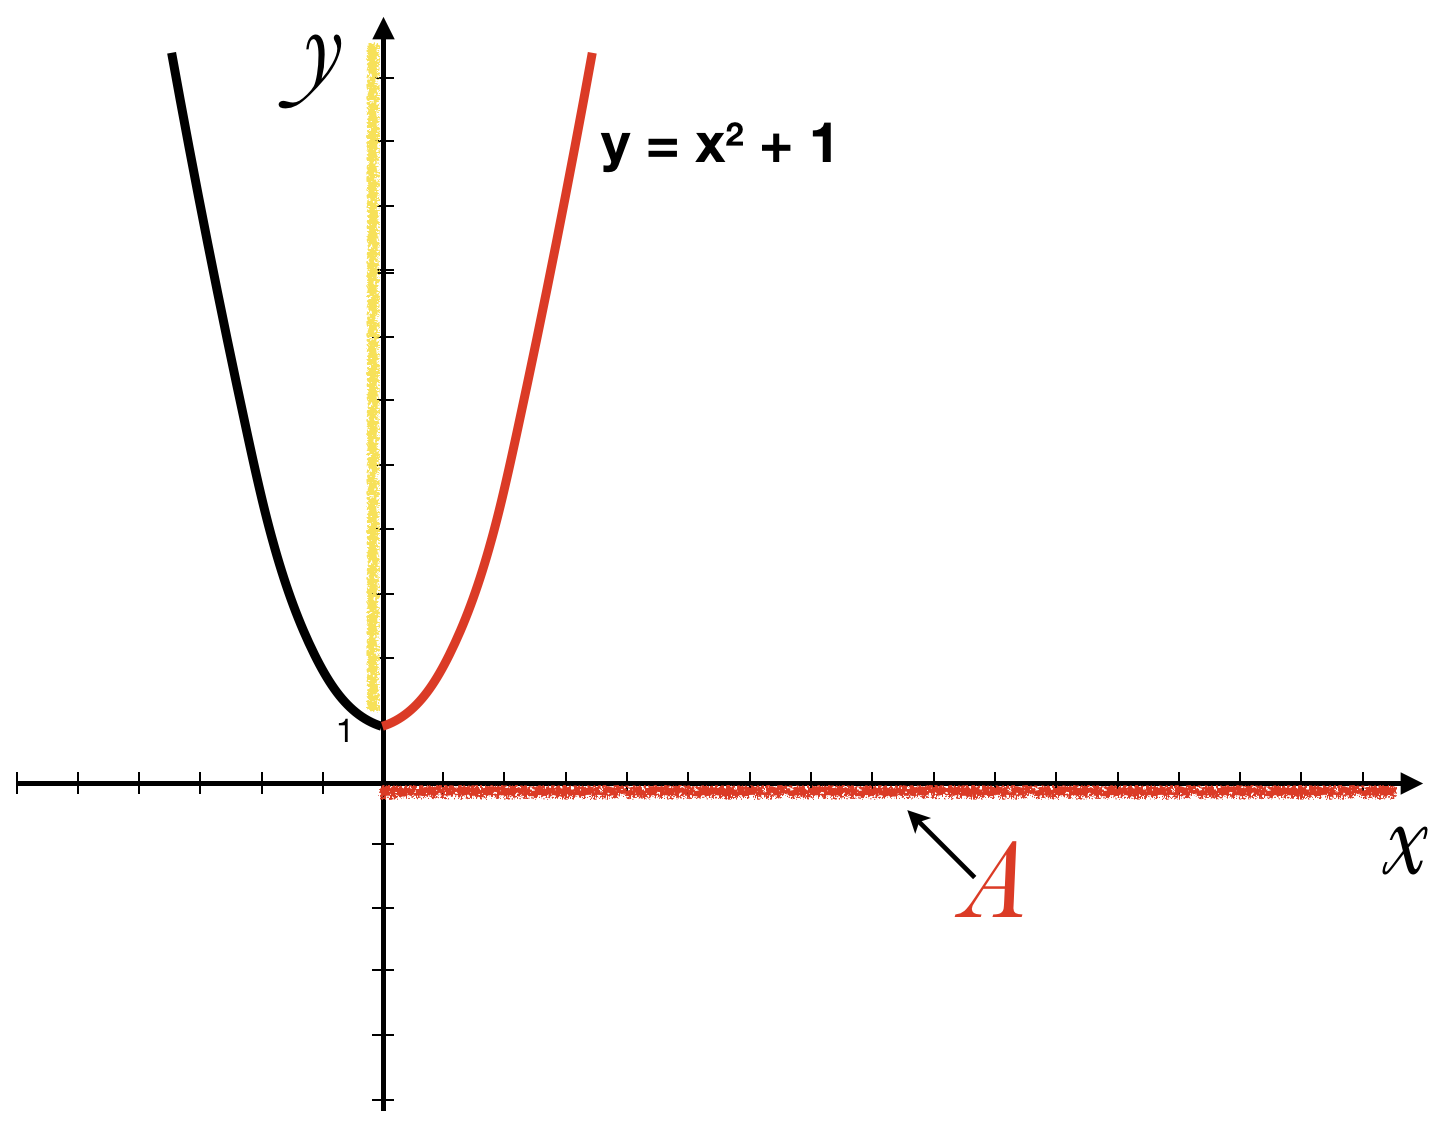
\includegraphics[width=0.7\textwidth]{img/funz_14b.png} %\quad
  
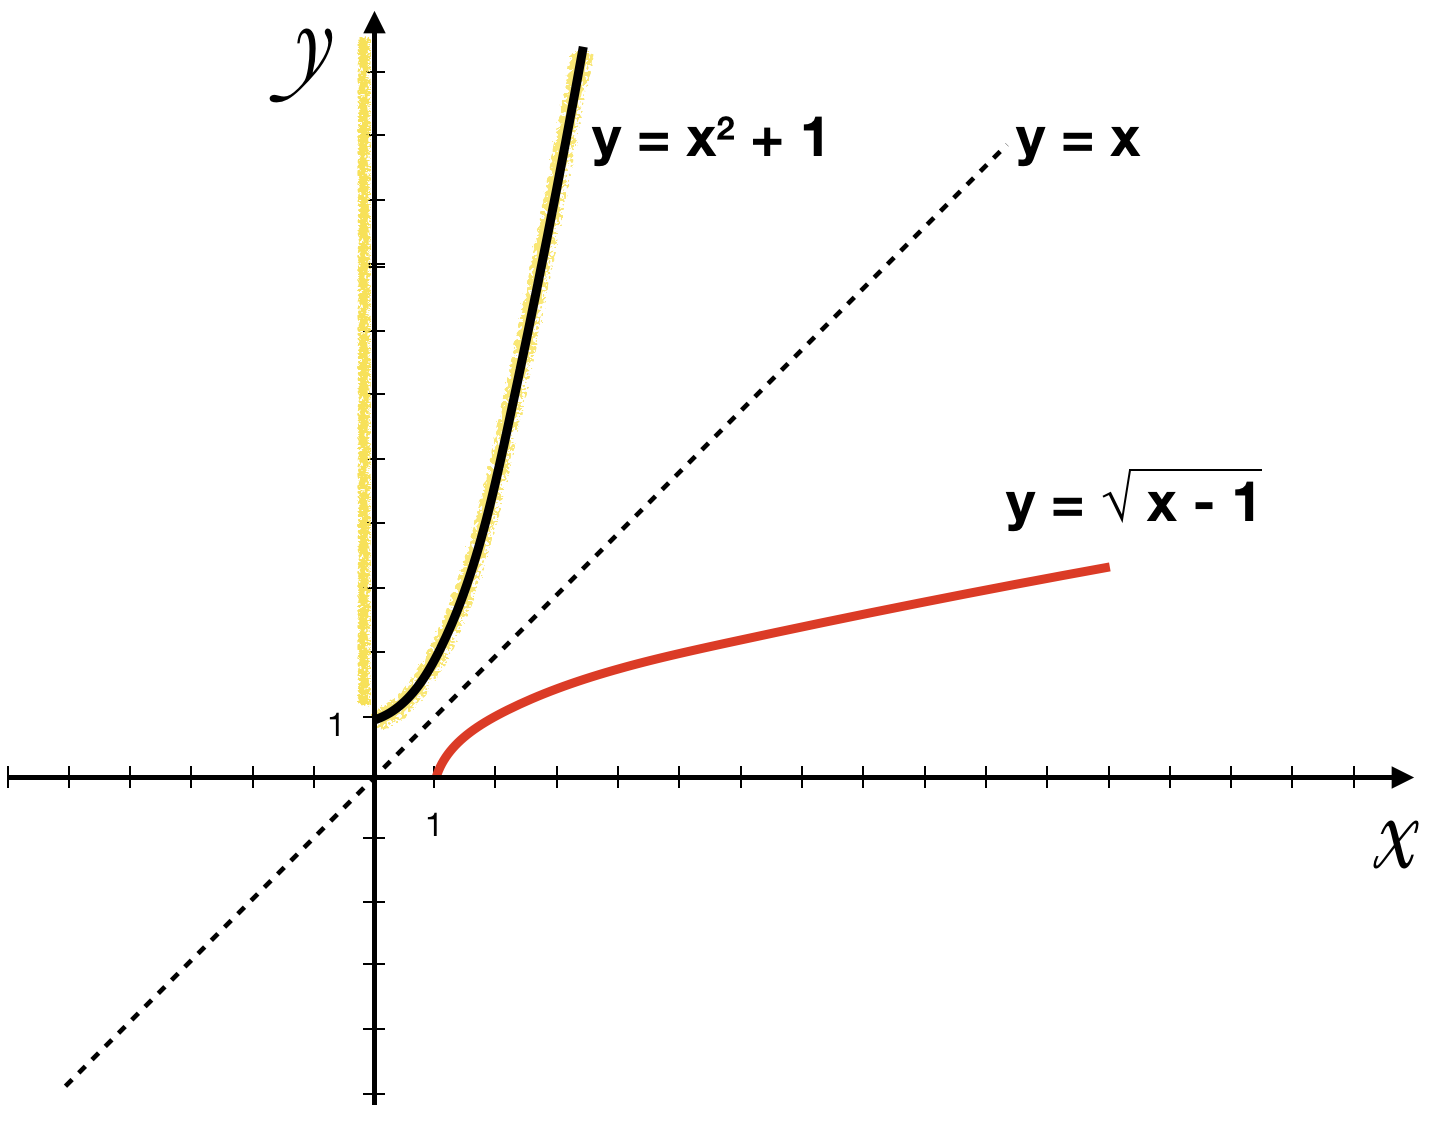
\includegraphics[width=0.45\textwidth]{img/funz_14c.png} 
  %\caption{}
  %\label{fig:funz_14abc}
  \end{figure}
\end{itemize}
\end{esempio}

Come visto negli esempi precedenti, il grafico della funzione $f^{-1}$, 
inversa della funzione $f$, è il simmetrico di $f$ rispetto alla bisettrice 
del primo e terzo quadrante.\\

Anche se sappiamo che l'inversa di una certa funzione deve essere simmetrica 
rispetto ad essa, trovare l'inversa di una determinata funzione e in 
particolar modo la sua forma analitica può non essere immediato. Forniamo 
quindi una procedura.\\

%\begin{procedura}
\textbf{Procedura 1.1} Determinare l'inversa di una funzione data:% 
\textcolor{blue}{[vedi la procedura a pag 100 vol3]}
\begin{enumerate}
  \item Si verifica che $f(x)$ è invertibile;
  \item Si esplicita la $f$ rispetto a $x$;
  \item Nella forma appena trovata si sostituisce $x$ con $y$ e $y$ con 
$x$.
\end{enumerate}
%end{procedura}
  
\begin{esempio}
Invertiamo la funzione: $f(x)=y=\sqrt[3]{x}-1$
\begin{enumerate}
  \item La funzione è invertibile perché è strettamente crescente in 
tutto il dominio $\mathbb{R}$.
  \item Esplicitiamo la funzione rispetto a $x$:\\
   $y=\sqrt[3]{x}-1\rightarrow y+1=\sqrt[3]{x}\rightarrow(y+1)^3=x$
  \item Infine otteniamo: $f^{-1}(x)=y=(x+1)^3$
\end{enumerate}
\end{esempio}

\begin{esempio}
Invertiamo la funzione: $f(x)=y=e^{x+1}-1$
\begin{enumerate}
  \item La funzione è invertibile perché è strettamente crescente in 
$\mathbb{R}$.
  \item Esplicitiamo la funzione rispetto a $x$:\\
   $y=e^{x+1}-1\rightarrow y+1=e^{x+1}\rightarrow 
\ln(x+1)=\ln(e^{x+1})\rightarrow \ln(y+1)-1=x$.\item Infine otteniamo: 
$f^{-1}(x)=y=\ln(x+1)-1$.
\end{enumerate}
\end{esempio}

Studiate le funzioni inverse discutiamo ora un'operazione tra funzioni che ci 
consentirà di creare funzioni complesse a partire da funzioni semplici: 
questa operazione si chiama \textsc{composizione di funzioni} e il suo 
risultato sarà una nuova funzione detta composta.\\

%
\begin{definizione} 
Date le funzioni $f : A\to B$ e $g : B\to C$ si dice funzione composta 
$f\circ g$ la funzione:   $(g\circ f)(x)=g(f(x))$ che associa ad ogni 
elemento di $A$ un elemento di $C$ in modo che
  \begin{itemize}
  \item all'elemento $x\in A$ corrisponde mediante $f$, 
l'elemento $f(x)\in B$
  \item all'elemento $f(x)\in B$ corrisponde, mediante $g$, 
l'elemento $g(f(x))\in C$
  \end{itemize}
affinché sia possibile calcolare $g(f(x))$, $f(x)$ deve appartenere al 
dominio di $g$. Il dominio di $g\circ f$ è costituito da tutti gli elementi 
del dominio di $f$ tali che $f(x)$ appartiene al dominio di $g$.
\end{definizione}

\begin{figure}[htpb!]
  \centering
  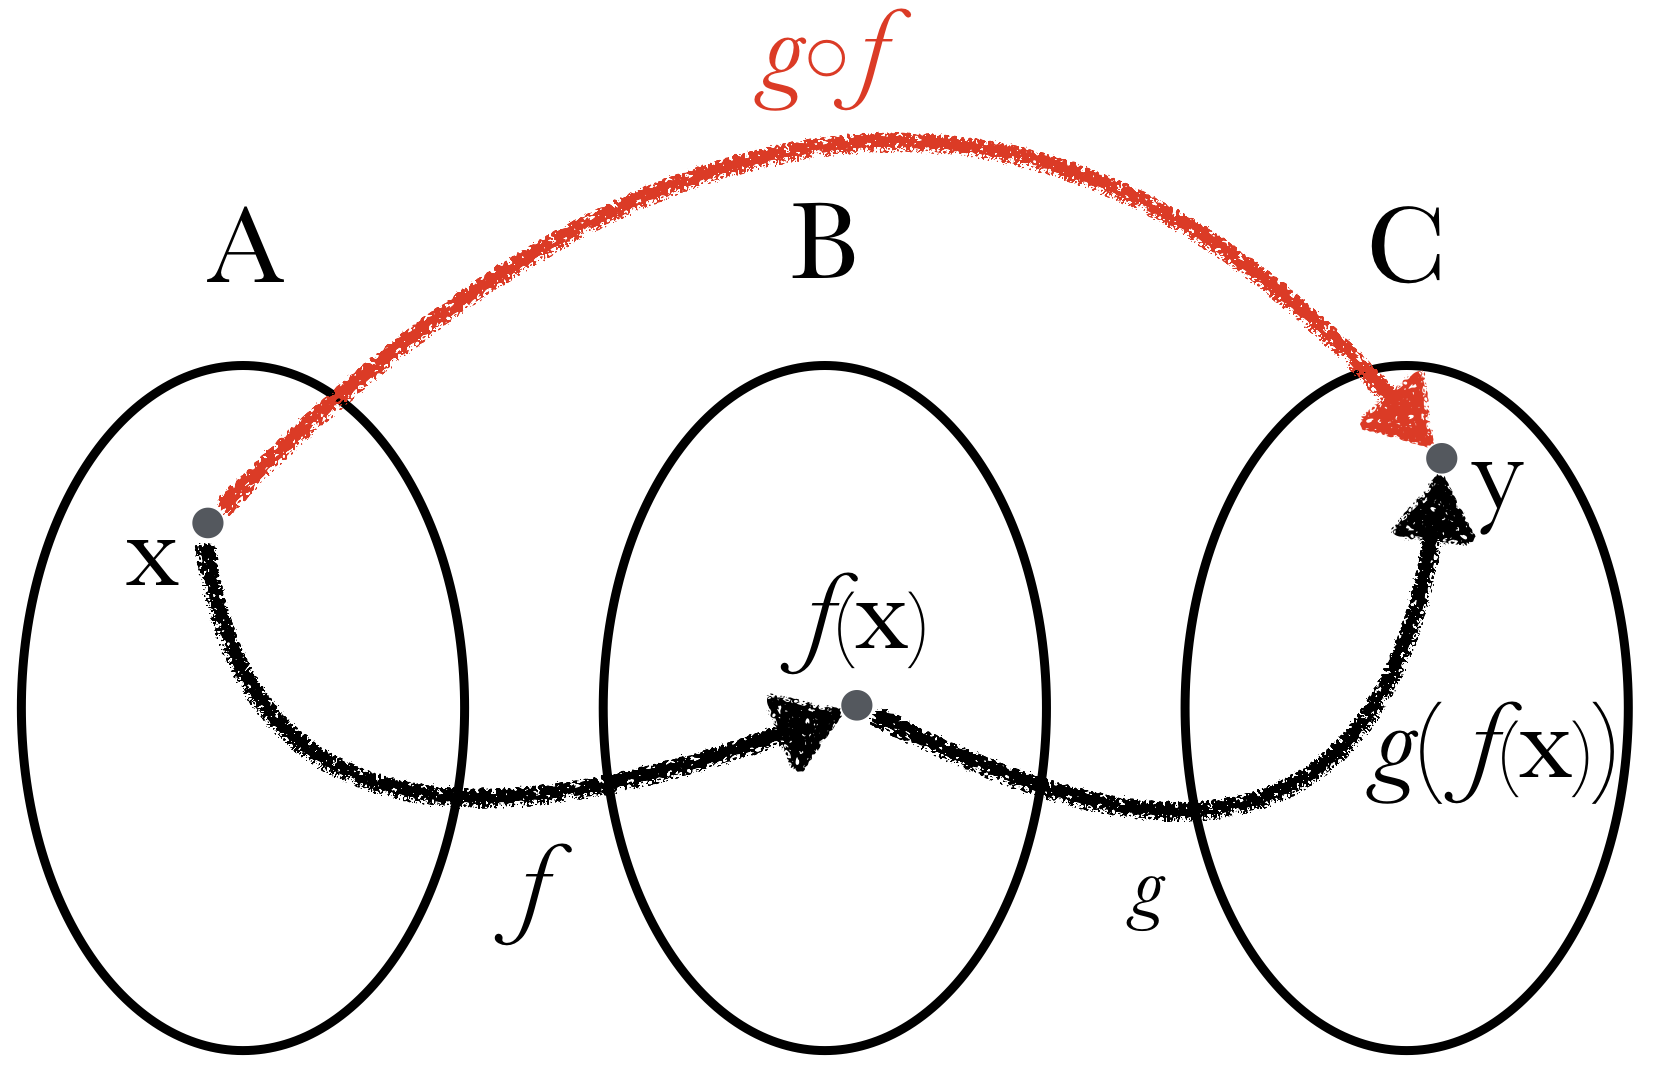
\includegraphics[width=0.55\textwidth]{img/funz_15.png} 
  %\caption{}
  %\label{fig:funz_14abc}
\end{figure}
%

La simbologia $g\circ f$ si legge <<$g$ composto $f$>> o <<$g$ dopo $f$>>; 
$g(f(x))$ si legge <<$g$ di $f$ di $x$>>.\\
 
Per quanto riguarda le proprietà di questa operazione tra funzioni notiamo 
che la composizione è associativa: $(f\circ g)\circ h=f\circ (g\circ h)$, ma 
in generale non commutativa $g\circ f\neq f\circ g.$ \\

\begin{esempio} 
Date le due funzioni $f(x)=\sqrt{x}$ e $g(x)= x+5$, determiniamo le funzioni 
composte $g\circ f$ e $f\circ g$.
Abbiamo $g\circ f=g(f(x))=g(\sqrt{x})=\sqrt{x}+5$ e il dominio  della 
funzione ottenuta è $x\geq0$. Otteniamo l'altra composta con un procedimento 
analogo $f\circ g=f(g(x))=f(x+5)=\sqrt{x+5}$ e il suo dominio è $x\geq5$. La 
diversità delle due funzioni ottenute ci conferma la non commutatività 
dell'operazione di composizione.\\
\end{esempio}

\textbf{Posso comporre una funzione con la sua inversa?}\\
Sia $f$ una funzione invertibile di dominio $D$ e immagine $I$, con $f^{-1} $ 
la sua inversa.
Consideriamo la composta $f^{-1}\circ f$, cioè $f^{-1}$ dopo $f$: $x$ va in 
$f(x)$ che a sua volta va in $x$, $f^{-1}(f(x))=x$, $\forall x\in D$ 
$f^{-1}\circ f$ è la funzione identità in $D$, analogamente anche 
$f(f^{-1}(x))=x$, $f\circ f^{-1}$ è l'identità in $I$. Ricordiamo che la 
funzione identità è una particolare funzione che associa ad ogni $x$ la $x$ 
stessa, cioè associa ad ogni elemento del dominio, lo stesso elemento nel 
codominio.\\

\begin{definizione}
Due funzioni $f$ e $g$ si dicono uguali se hanno lo stesso dominio $D$ e 
risulta $$f(x)=g(x)$$ $\forall x\in D$.\\
\end{definizione}
 
\begin{esempio}
Vediamo un esempio di funzioni uguali e non uguali. Le due funzioni
$$f(x)=\frac{\sqrt{x}}{\sqrt{x^2+4}}$$ e $$g(x)=\sqrt{\frac{x}{x^2+4}}$$
sono uguali perchè hanno lo stesso dominio ($x\geq0$) e risulta:
$$\frac{\sqrt{x}}{\sqrt{x^2+4}}=\sqrt{\frac{x}{x^2+4}}$$ per ogni $x\geq0$.
Vediamo un contoesempio di funzioni uguali. Le due funzioni
$$f(x)=\frac{\sqrt{x}}{\sqrt{x+4}}$$ e $$g(x)=\sqrt{\frac{x}{x+4}}$$
non sono uguali perché hanno dominio diverso: la funzione $f$ è definita per 
$x\geq0$, mentre la funzione $g$ è definita per $x<-4\lor x\geq 0$.
$$\frac{\sqrt{x}}{\sqrt{x^2+4}}=\sqrt{\frac{x}{x^2+4}}$$ per ogni $x\geq0$.
\end{esempio}


\end{comment}








